\chapter{Information Theory}
\label{ch:infotheory}

\begin{chapterintro}
Every other chapter of this book asks how to \emph{build} a communication system. This one asks
what is \emph{possible}, whatever you build. In 1948 a 32-year-old mathematician at Bell Labs who
juggled, rode a unicycle and built a mechanical mouse that could learn a maze showed that
information can be measured like water or electricity; that every source has an irreducible
rate, its \emph{entropy}; and that every channel has a hard speed limit, its \emph{capacity},
below which you can communicate as reliably as you like and above which you cannot. The chapter
builds those ideas from the ground up, with pictures wherever the mathematics allows: surprise
and entropy, mutual information, long typical sequences and compression, channels and the
coding theorem, the error exponent and the short-packet penalty, the Gaussian channel and its
famous formula $C=B\log_2(1+\mathrm{SNR})$ derived by packing oranges in a thousand
dimensions, the $-1.59$\,dB Shannon limit, real constellations and shaping, water-filling,
fading, MIMO, many users, rate--distortion and secrecy. It closes by placing today's systems,
from DVB-S2 to 5G, against the limits, and tells the story of a fifty-year chase in which
engineers took Shannon's existence proof and, one decibel at a time, built codes that reach it.
\end{chapterintro}

%======================================================================
\section{Measuring information}
\label{sec:ch13:intro}
%======================================================================

Ask a working engineer what a communication link does and you will hear about volts, hertz,
decibels and bit error rates. Ask what it \emph{carries} and the answer becomes slippery. A
telephone line carries speech; a satellite carries television; a fibre carries packets. A
telegraph wire in 1900 carried dots and dashes, and a deep-space antenna today carries
photographs of Neptune's moons. Is there one commodity under all of these?

Claude Shannon's great insight was that there is, and that it can be measured with a single
number, independent of what the message means, what the channel is made of and how the engineer
chooses to modulate it. Once information has a unit, a channel has a capacity in that unit, just
as a pipe has a capacity in litres per second, and design becomes the art of approaching that
capacity at acceptable cost. Figure~\ref{fig:ch13_timeline} shows how quickly that one idea grew
into a field, and how long it took engineering to catch up with it.

\mdcfig{ch13_timeline}{Information theory at a glance. The ingredients (Nyquist, Hartley,
Kotelnikov) were in place by the 1930s; Shannon's 1948 paper (red) assembled them into a theory;
the next sixty years were spent building codes, algorithms and multi-user results that turned its
promises into hardware. Every name on this line appears later in the chapter.}

\subsection{Before Shannon: Nyquist, Hartley and Kotelnikov}

The idea that information could be counted grew out of telegraphy, the first industry that sold
messages by the word. In 1924 Harry Nyquist, in ``Certain factors affecting telegraph speed'',
asked how fast a line of given bandwidth could send telegraph signals and argued that the speed
was proportional to the logarithm of the number of distinguishable current values. His 1928 paper,
which we met in Chapter~\ref{ch:baseband}, showed that a channel of bandwidth $B$ can carry at most
$2B$ independent pulse amplitudes per second.

In the same year Ralph Hartley, also at Bell Labs, published ``Transmission of Information''. He
argued that a quantitative measure of information should ignore ``psychological factors'' and
depend only on the number of possible messages. Think of it as counting the doors a message could
have walked through. If each of $n$ selections is made from an alphabet of $s$ symbols, there are
$s^n$ possible messages, and Hartley defined the information as
\begin{equation}
H_{\text{Hartley}}=\log s^n=n\log s.
\label{eq:ch13:hartley}
\end{equation}
The logarithm is the key move: it makes information \emph{additive}. Two telegrams carry twice
as much as one, even though the number of possible pairs is the square of the number of singles.
Combining Hartley's measure with Nyquist's $2B$ pulses per second, and a number of distinguishable
levels $M$ limited by noise, gives a rate proportional to $2B\log_2 M$, and engineers of the 1930s and
1940s used ``Hartley's law'' informally in exactly that way.

What Hartley's measure lacked was any notion of \emph{probability}. It treats every message as
equally likely---``the train is on time'' and ``the bridge has collapsed'' count the same---and it
says nothing about noise except that noise limits the number of levels. In the Soviet Union,
Vladimir Kotelnikov proved the sampling theorem in 1933, independently of Whittaker, Nyquist and
later Shannon, and in his 1947 doctoral thesis on the ``potential noise immunity'' of signals he
developed the geometric, signal-space view of optimum detection that Chapter~\ref{ch:modulation}
uses. By the mid-1940s, then, the ingredients were on the bench: bandwidth sets the number of
dimensions per second, noise sets how finely each can be divided, and logarithms turn counts into
additive measures. Nobody had yet put them together into a theory with theorems.

\begin{figure}[htbp]\centering
\begin{minipage}[t]{0.36\linewidth}\centering
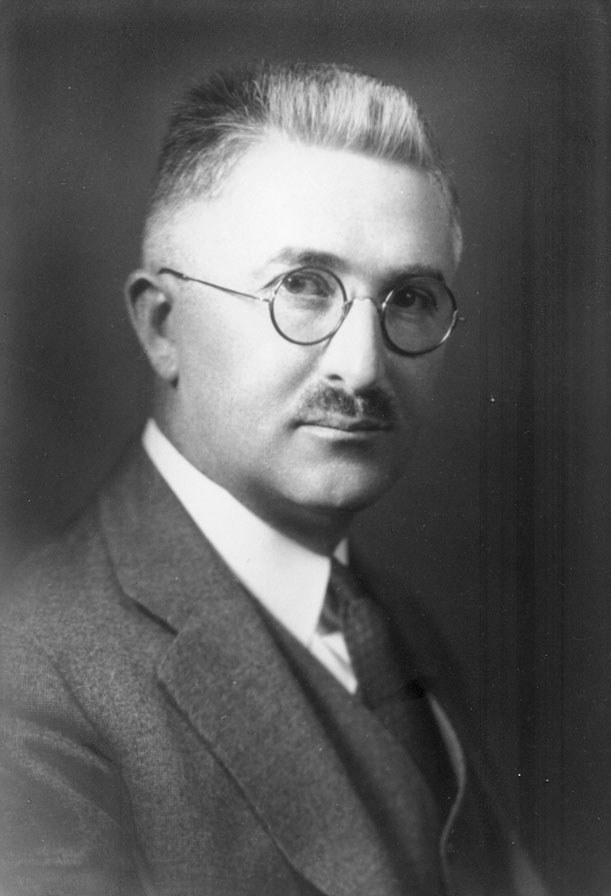
\includegraphics[width=\linewidth,height=5.4cm,keepaspectratio]{figs/photos/ch13_hartley}
\caption{Ralph V.\,L. Hartley, whose 1928 paper first proposed the logarithm of the number of
possible messages as a measure of information.\mdccredit{ch13_hartley}}
\label{fig:ch13_hartley}\end{minipage}\hfill
\begin{minipage}[t]{0.6\linewidth}\centering
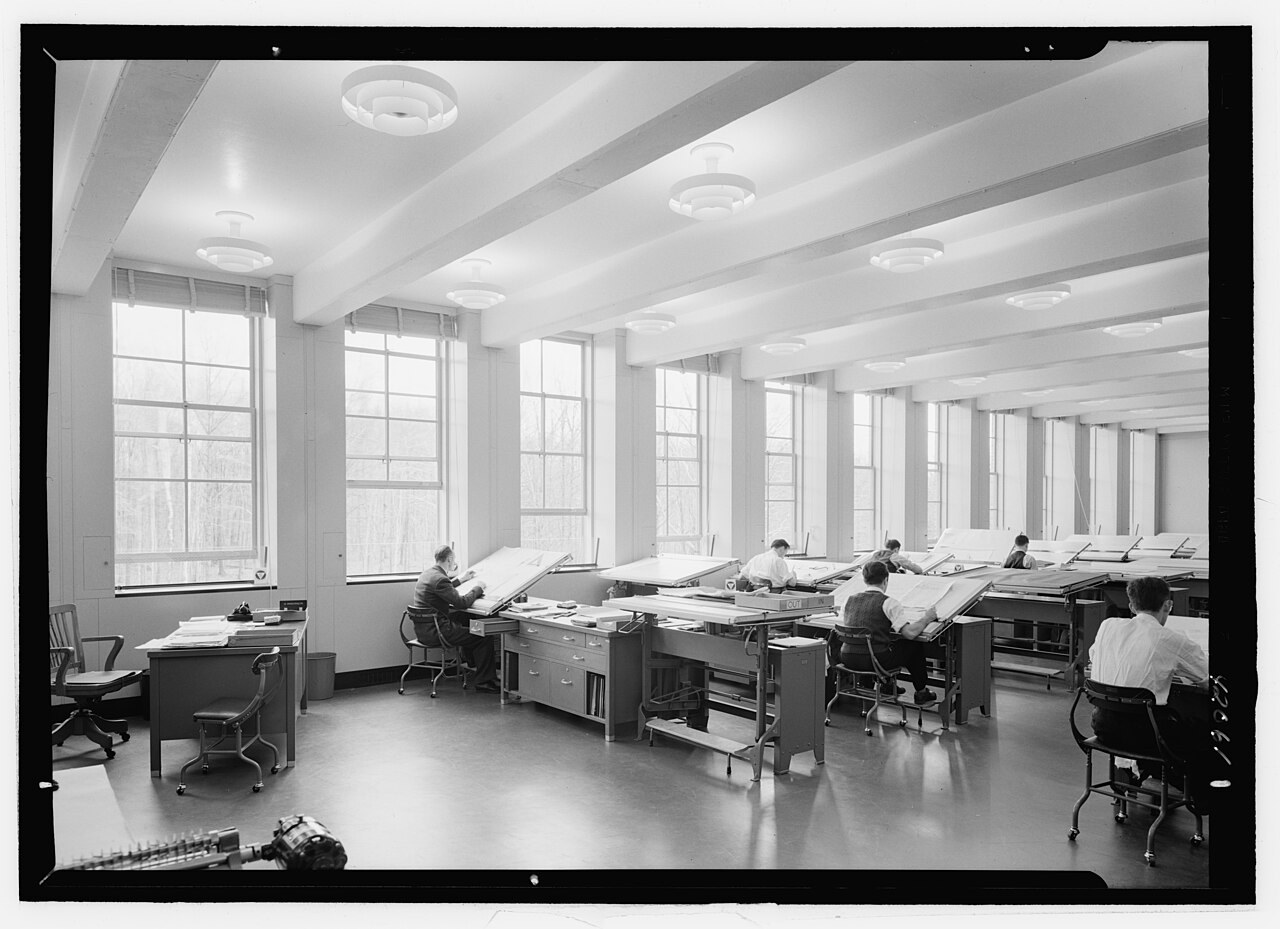
\includegraphics[width=\linewidth,height=5.4cm,keepaspectratio]{figs/photos/ch13_bell_labs}
\caption{A drafting room at Bell Telephone Laboratories, Murray Hill, New Jersey, in 1942
(Gottscho-Schleisner photograph). Shannon joined Bell Labs in 1941, and the Murray Hill
campus was the birthplace of the transistor.\mdccredit{ch13_bell_labs}}
\label{fig:ch13_bell_labs}\end{minipage}
\end{figure}

\begin{history}[Shannon at Bell Labs]
Claude Elwood Shannon was born in 1916 in Petoskey, Michigan, and grew up in the small town of
Gaylord, where he built model aeroplanes and a barbed-wire telegraph to a friend's house half a
mile away. His 1937 MIT master's thesis showed that Boolean algebra could describe and simplify
relay switching circuits---arguably the most consequential master's thesis of the century, since
it founded digital circuit design. After a PhD on the algebra of genetics and a year at the
Institute for Advanced Study, he joined Bell Telephone Laboratories in 1941. There he worked on
fire-control systems and on cryptography, the latter leading to a classified 1945 report on the
mathematics of secrecy. He met Alan Turing, visiting Bell Labs in 1943 to review the laboratory's
speech-encryption work, and the two talked over lunch about machines that could think. Shannon's
cryptographic work fed directly into the theory of communication; he later said the two were so
close that he could not separate them.

``A Mathematical Theory of Communication'' appeared in two parts in the \emph{Bell System
Technical Journal} in July and October 1948. Its opening states the problem with a clarity that
has never been bettered: ``The fundamental problem of communication is that of reproducing at
one point either exactly or approximately a message selected at another point.'' Shannon then
set meaning aside---``these semantic aspects of communication are irrelevant to the engineering
problem''---and in some 80 pages defined entropy, proved the source coding theorem, defined
channel capacity, proved the noisy channel coding theorem, derived the capacity of the
band-limited Gaussian channel and sketched rate--distortion theory. The word \emph{bit}, a
contraction of ``binary digit'', appeared in print for the first time in the paper; Shannon
credited it to his colleague John Tukey.
\end{history}

\mdcphoto[0.3]{ch13_shannon_statue}{Claude Shannon (1916--2001), in bronze at AT\&T's Shannon
Laboratory (one of several statues of him by the sculptor Eugene Daub). In one paper he gave
engineering its unit of information, its speed limit and its proof that the limit can be
reached.}

\subsection{The playful genius}

It is easy to imagine the author of the most abstract paper in engineering as a remote
theoretician. Shannon was the opposite: a tinkerer who thought with his hands. Colleagues at Bell
Labs remembered him riding a unicycle down the corridors, sometimes juggling as he went, and he
later built machines to juggle for him (Figure~\ref{fig:ch13_juggler}). He even worked out a
small ``theorem'' of juggling relating how long the balls spend in the air and in the hands. At
home he built a calculator that worked in Roman numerals, a flame-throwing trumpet, and a box
whose only function, when you flipped its switch, was to open its lid, extend a hand and switch
itself off.

The toy that mattered most was \emph{Theseus} (Figure~\ref{fig:ch13_theseus}), built around
1950: a small mechanical mouse, moved by electromagnets under the floor of a reconfigurable maze
and controlled by a few dozen telephone relays. Released into an unfamiliar maze, Theseus explored
by trial and error until it reached the ``cheese''; put back at the start, it ran straight to the
goal, because the relays remembered the right turn at every square. Change the maze and it
relearned. It is often cited as one of the first machines that learned from experience, and it
shows the habit of mind behind the 1948 paper: take a vague question (\emph{can a machine learn?
how much can a wire carry?}), strip it to its skeleton, and build the simplest thing that answers
it.

\begin{figure}[htbp]\centering
\begin{minipage}[t]{0.58\linewidth}\centering
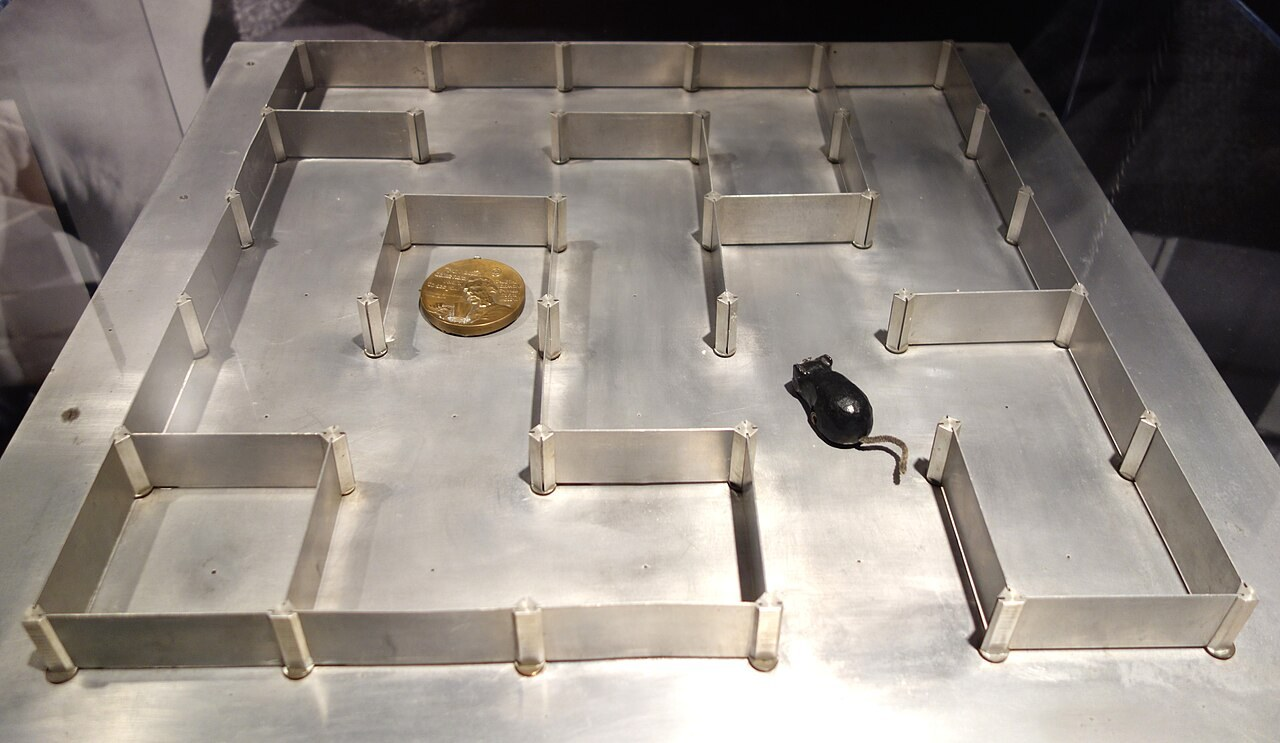
\includegraphics[width=\linewidth,height=5.0cm,keepaspectratio]{figs/photos/ch13_theseus}
\caption{Shannon's Theseus maze (1952 version, MIT Museum). The mouse is moved by a magnet on a
carriage under the floor; banks of relays below remember which way it left each square on its
last successful run.\mdccredit{ch13_theseus}}
\label{fig:ch13_theseus}\end{minipage}\hfill
\begin{minipage}[t]{0.38\linewidth}\centering
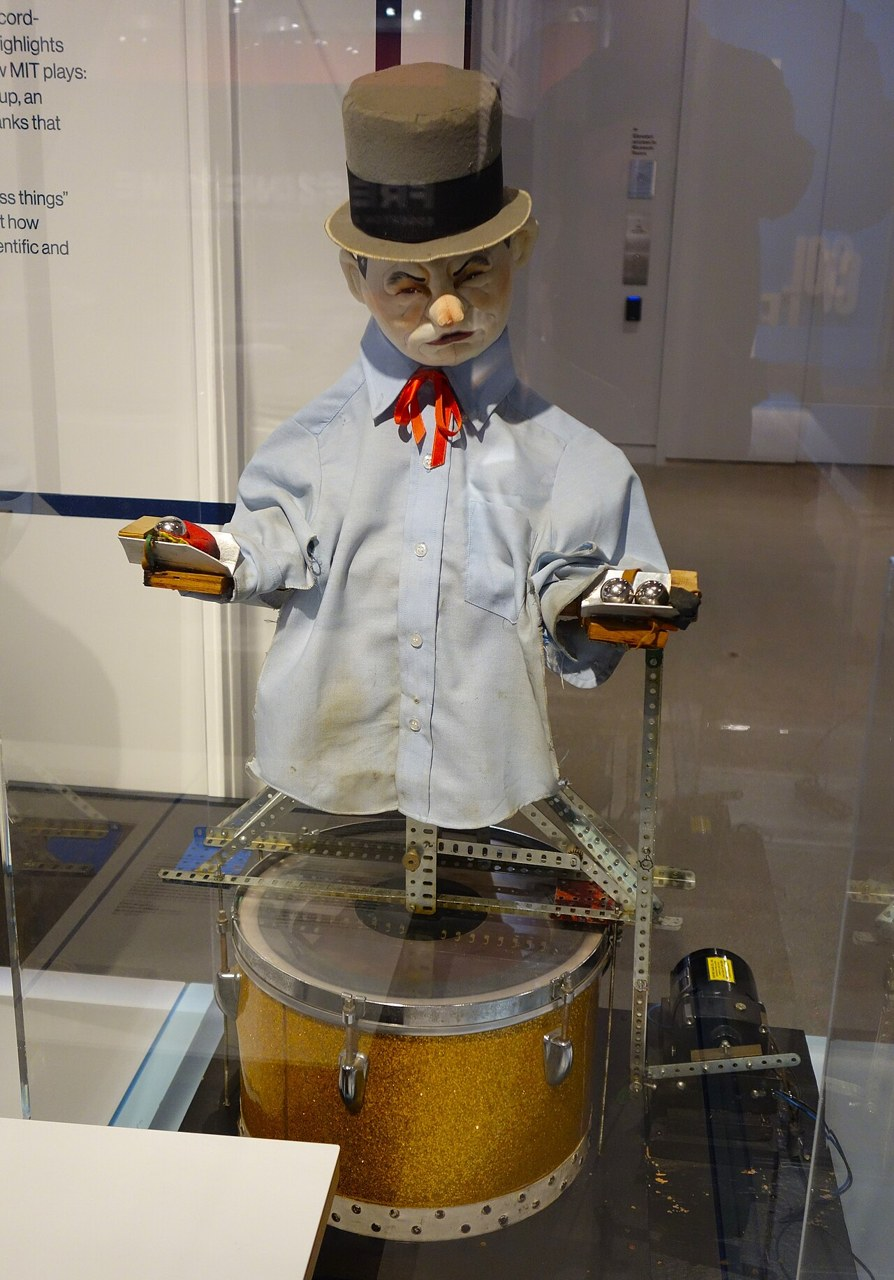
\includegraphics[width=\linewidth,height=5.0cm,keepaspectratio]{figs/photos/ch13_juggler}
\caption{One of Shannon's juggling machines, a bounce-juggling ``W.\,C. Fields'' figure from the
early 1980s, now at the MIT Museum.\mdccredit{ch13_juggler}}
\label{fig:ch13_juggler}\end{minipage}
\end{figure}

\subsection{Shannon's model}

Shannon's block diagram, reproduced in Figure~\ref{fig:ch01:shannon} of Chapter~\ref{ch:history}
and redrawn in Figure~\ref{fig:ch13_model}, separates the source, the transmitter, the channel with
its noise, the receiver and the destination. The key modelling decision is to treat the source as
a \emph{random process}. From the engineer's point of view the message to be sent is unknown; if it
were known in advance there would be no need to send it. Information is therefore tied to
uncertainty, and uncertainty is measured with probability. The channel, likewise, is described by
the conditional probability of its output given its input. Everything else---how the message is
coded, what waveforms are used, how the receiver decides---is left free, and the theorems speak
about the best that \emph{any} choice could achieve.

\begin{figure}[htbp]\centering
\begin{tikzpicture}[node distance=0.5cm and 0.55cm,
  blk/.style={draw=navy,fill=navy!6,thick,minimum height=1.0cm,minimum width=1.65cm,align=center,font=\sffamily\scriptsize},
  arr/.style={-{Stealth[length=2mm]},thick,navy}]
\node[blk] (s) {Information\\source};
\node[blk,right=of s] (t) {Transmitter\\(source + channel\\encoder)};
\node[blk,right=0.9cm of t,fill=accent!8,draw=accent] (c) {Channel\\$W(y\mid x)$};
\node[blk,right=0.9cm of c] (r) {Receiver\\(decoders)};
\node[blk,right=of r] (d) {Destination};
\node[blk,below=0.55cm of c,fill=accent!8,draw=accent,minimum height=0.7cm] (n) {Noise source};
\draw[arr] (s) -- node[above,font=\scriptsize]{$W$} (t);
\draw[arr] (t) -- node[above,font=\scriptsize]{$X^n$} (c);
\draw[arr] (c) -- node[above,font=\scriptsize]{$Y^n$} (r);
\draw[arr] (r) -- node[above,font=\scriptsize]{$\hat W$} (d);
\draw[arr,accent] (n) -- (c);
\node[below=0.15cm of s,font=\sffamily\scriptsize,text=gray,align=center] {entropy rate $\mathcal{H}$};
\node[below=0.15cm of t,font=\sffamily\scriptsize,text=gray,align=center] {rate $R$};
\node[below=0.15cm of r,font=\sffamily\scriptsize,text=gray,align=center] {$P_e\to0$?};
\end{tikzpicture}
\caption{Shannon's model of communication, labelled with the quantities of this chapter. The
source is summarised by one number (its entropy rate $\mathcal{H}$), the channel by one number
(its capacity $C$); reliable communication is possible exactly when $\mathcal{H}<C$.}
\label{fig:ch13_model}
\end{figure}

\begin{keyidea}[Separate what from how]
Information theory characterises a source by one number (its entropy rate) and a channel by one
number (its capacity), both independent of implementation. The \emph{source--channel separation
theorem} (Section~\ref{sec:ch13:rd}) then says that, for long messages, nothing is lost by
designing the compression and the error-control coding separately and connecting them through a
stream of bits. That is why the digital world could standardise on the bit as a universal
interface: the same fibre carries voice, video and data, and the codec designers never need to
talk to the modem designers.
\end{keyidea}

%======================================================================
\section{Entropy}
\label{sec:ch13:entropy}
%======================================================================

\subsection{Information is surprise}

Imagine two weather forecasters. One works in the middle of the Sahara, the other in London.
Every morning each announces ``rain'' or ``no rain''. The Saharan forecaster says ``no rain''
almost every day, and you barely listen: you knew that already. The day she says ``rain'',
everyone stops what they are doing. The London forecaster's announcement is useful every single
day, because you genuinely could not have guessed it.

That is the whole intuition behind Shannon's measure. Information is \emph{surprise}. A message
that you could have predicted tells you little; a message that overturns your expectations tells
you a lot. A good newspaper editor knows this instinctively: ``dog bites man'' is not news, ``man
bites dog'' is.

\mdcfig[0.5]{ch13_surprise}{The surprise ladder: self-information $\log_2(1/p)$ of some everyday
events. Halving the probability adds exactly one bit. The probabilities of weather are
illustrative; the card and lottery odds are exact.}

Suppose a source emits one of a finite set of symbols $x$ with probabilities $p(x)$. How much
information does the occurrence of a particular symbol convey? Shannon asked what properties such
a measure $I(x)$ should have. It should depend only on the probability, $I(x)=f(p(x))$; it
should be larger for rarer events (learning that the sun rose this morning tells you little;
learning that your lottery ticket won tells you a lot); a certain event should carry no
information, $f(1)=0$; and the information from two independent events should add,
$f(pq)=f(p)+f(q)$. Only one family of continuous functions passes all four tests: the
logarithm. So the \term{self-information} of an outcome is
\begin{equation}
I(x)=\log_2\frac{1}{p(x)}\quad\text{bits}.
\label{eq:ch13:selfinfo}
\end{equation}
Read it as ``how many times would you have to halve the odds to get down to this event?''. The
base of the logarithm fixes the unit: base 2 gives \term{bits} (also called shannons), natural
logarithms give \emph{nats} ($1\ \text{nat}=1.443\ \text{bits}$), and base 10 gives hartleys. A
fair coin toss carries $\log_22=1$ bit; one card drawn from a shuffled deck carries
$\log_252=5.7$ bits; an event with probability one in a million carries 19.9 bits
(Figure~\ref{fig:ch13_surprise}).

\subsection{The entropy of a source: a game of twenty questions}

A single surprise is interesting; an engineer needs an \emph{average}. The \term{entropy} of a
discrete random variable $X$ is its average self-information,
\begin{equation}
H(X)=\E\!\left[\log_2\frac{1}{p(X)}\right]=-\sum_x p(x)\log_2p(x)\quad\text{bits},
\label{eq:ch13:entropy}
\end{equation}
with the convention $0\log0=0$ (an impossible symbol contributes nothing). Entropy measures the
average uncertainty about $X$ before it is observed, or equivalently the average information
gained when it is.

\begin{figure}[htbp]\centering
\begin{tikzpicture}[
  q/.style={draw=navy,fill=navy!6,thick,rounded corners=3pt,align=center,font=\sffamily\scriptsize,minimum height=0.75cm},
  leaf/.style={draw=practc,fill=practc!10,thick,rounded corners=3pt,align=center,font=\sffamily\scriptsize,minimum width=1.6cm,minimum height=0.7cm},
  e/.style={-{Stealth[length=1.6mm]},thick,navy!70},
  lab/.style={font=\sffamily\scriptsize\bfseries,text=accent}]
\node[q] (q1) at (0,0) {Q1: Is it clear?};
\node[leaf] (c) at (-2.6,-1.3) {clear ($\tfrac12$)\\code \texttt{0}};
\node[q] (q2) at (1.6,-1.3) {Q2: Is it cloudy?};
\node[leaf] (cl) at (-0.6,-2.6) {cloudy ($\tfrac14$)\\code \texttt{10}};
\node[q] (q3) at (3.2,-2.6) {Q3: Is it rain?};
\node[leaf] (r) at (1.4,-3.9) {rain ($\tfrac18$)\\code \texttt{110}};
\node[leaf] (s) at (5.0,-3.9) {snow ($\tfrac18$)\\code \texttt{111}};
\draw[e] (q1) -- node[lab,above left]{yes = 0} (c);
\draw[e] (q1) -- node[lab,above right]{no = 1} (q2);
\draw[e] (q2) -- node[lab,above left]{yes = 0} (cl);
\draw[e] (q2) -- node[lab,above right]{no = 1} (q3);
\draw[e] (q3) -- node[lab,above left]{yes = 0} (r);
\draw[e] (q3) -- node[lab,above right]{no = 1} (s);
\node[font=\sffamily\scriptsize,align=left,anchor=west] at (5.2,-0.6)
 {average number of questions\\$=\tfrac12\cdot1+\tfrac14\cdot2+\tfrac18\cdot3+\tfrac18\cdot3$\\$=1.75=H$ bits};
\end{tikzpicture}
\caption{Twenty questions (well, three) for a weather station. Each answer is one bit; writing
the answers down gives a prefix code. Because every question splits the remaining probability
exactly in half, the average number of questions equals the entropy.}
\label{fig:ch13_questions}
\end{figure}

\begin{analogy}[Twenty questions]
In the parlour game, one player thinks of something and the others may ask only yes/no
questions. A good player does not ask ``Is it a giraffe?'' first; she asks questions that split
the remaining possibilities into two equally likely halves, because each such answer is worth
exactly one bit. Entropy is the number of yes/no questions that the \emph{best possible}
questioner needs, on average, to pin down the outcome. Twenty well-chosen questions can
distinguish $2^{20}\approx10^6$ things, which is why the game is hard to win but not hopeless.
The limit of the analogy: in the game you need a whole number of questions, whereas entropy can be
fractional; Section~\ref{sec:ch13:source} shows that by asking about \emph{long sequences} of
outcomes at once, the average number of questions per outcome comes as close to $H$ as you like.
\end{analogy}

Figure~\ref{fig:ch13_questions} plays the game for a weather station. Its basic properties follow
directly from the definition:
\begin{itemize}
\item $H(X)\ge0$, with equality only when $X$ is deterministic.
\item $H(X)\le\log_2|\mathcal{X}|$, where $|\mathcal{X}|$ is the alphabet size, with equality only
for the uniform distribution. (This follows from Jensen's inequality, or from the non-negativity
of relative entropy proved below.) Hartley's measure is therefore the special case of maximum
uncertainty.
\item Entropy depends only on the probabilities, not on the symbol values. Relabelling the
alphabet changes nothing.
\item For independent $X$ and $Y$, $H(X,Y)=H(X)+H(Y)$.
\end{itemize}

\begin{worked}[Entropy of a small source]
A weather station reports one of four conditions every hour: clear (probability $\frac12$),
cloudy ($\frac14$), rain ($\frac18$) and snow ($\frac18$). The entropy is
\[
H=\tfrac12\log_22+\tfrac14\log_24+\tfrac18\log_28+\tfrac18\log_28
=0.5+0.5+0.375+0.375=1.75\ \text{bits}.
\]
A naive fixed-length code needs two bits per report. The variable-length code
clear$\to$\texttt{0}, cloudy$\to$\texttt{10}, rain$\to$\texttt{110}, snow$\to$\texttt{111} has
average length $\frac12\cdot1+\frac14\cdot2+\frac18\cdot3+\frac18\cdot3=1.75$ bits, exactly the
entropy, and it is uniquely decodable because no codeword is a prefix of another. The match is
exact because every probability is a power of two, so every self-information is a whole number
of bits and each codeword length equals the self-information of its symbol. Section~\ref{sec:ch13:source}
shows that no uniquely decodable code can do better, and that for other distributions one can
always get within one bit (and, by coding blocks, arbitrarily close).
\end{worked}

For a binary source that emits a one with probability $p$, the entropy is the \term{binary
entropy function}
\begin{equation}
h(p)=-p\log_2p-(1-p)\log_2(1-p),
\label{eq:ch13:hb}
\end{equation}
plotted in Figure~\ref{fig:ch13_entropy}(a). It is symmetric about $p=\frac12$, where it reaches
one bit, and it falls steeply near the ends: a source that emits ones only 11\% of the time
carries only half a bit per symbol. Keep this function in your pocket. It will reappear as the
capacity of the binary symmetric channel, as the rate--distortion function of a binary source and
in the counting of binary sequences, because $\binom{n}{np}\approx2^{nh(p)}$ for large $n$.

\mdcfig{ch13_entropy}{(a) The binary entropy function $h(p)$. A fair coin carries one bit; a
coin that lands heads 11\% of the time carries half a bit. (b) Successive estimates of the
entropy of printed English with a 27-symbol alphabet (26 letters and a space), from Shannon's
1951 study: $F_0=\log_227$ assumes equiprobable letters, $F_N$ accounts for statistics of $N$-letter
blocks, and ``words'' uses word frequencies. Experiments in which people predicted the next letter
of a passage placed the long-range entropy between about 0.6 and 1.3 bits per letter.}

\subsection{How much information is in English?}

Look at a typewriter keyboard (Figure~\ref{fig:ch13_typewriter}) or a bag of Scrabble tiles and you
are looking at a statistical study of English. Scrabble's inventor, Alfred Butts, is said to have
fixed the number of tiles of each letter by counting letters in newspaper text; the rarest letters
(Q, Z) are given the highest scores. Telegraph operators knew the same statistics through their
fingers, as the In Practice box below explains.

\begin{figure}[htbp]\centering
\begin{minipage}[t]{0.55\linewidth}\centering
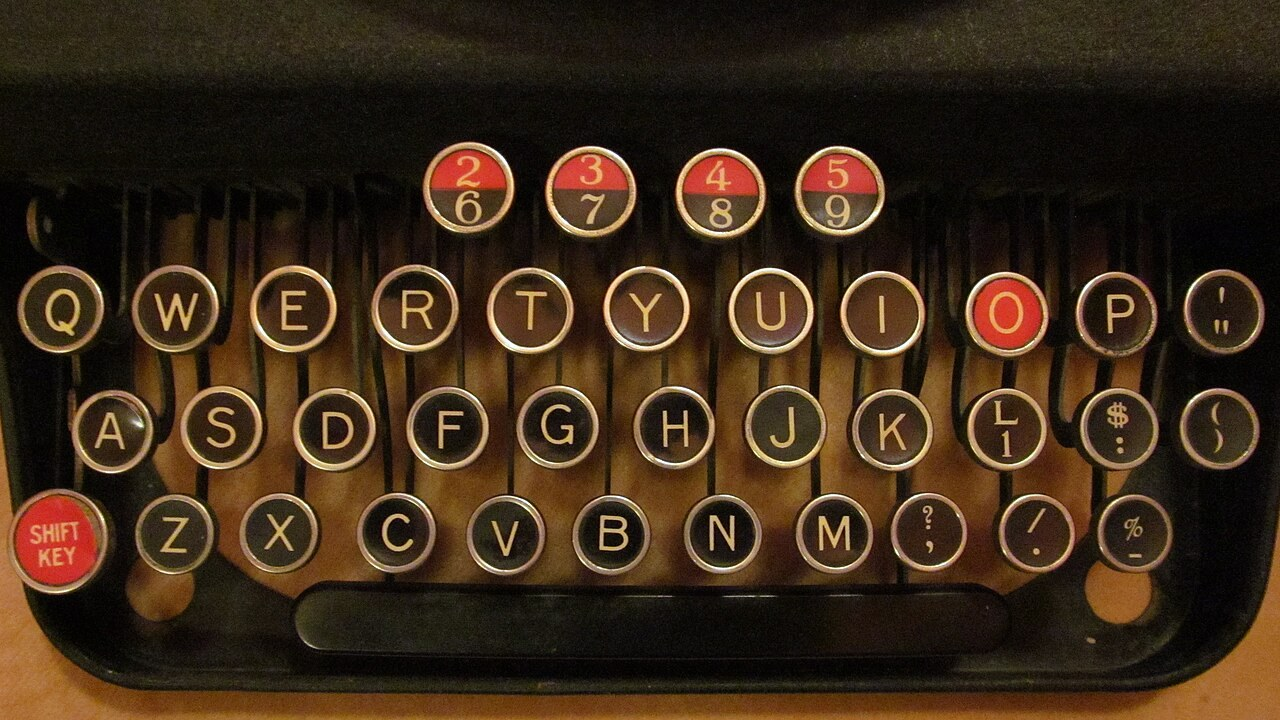
\includegraphics[width=\linewidth,height=4.6cm,keepaspectratio]{figs/photos/ch13_typewriter}
\caption{A mechanical typewriter keyboard. Every key is equally easy to make; the text that flows
through it is anything but uniform.\mdccredit{ch13_typewriter}}
\label{fig:ch13_typewriter}\end{minipage}\hfill
\begin{minipage}[t]{0.41\linewidth}\centering
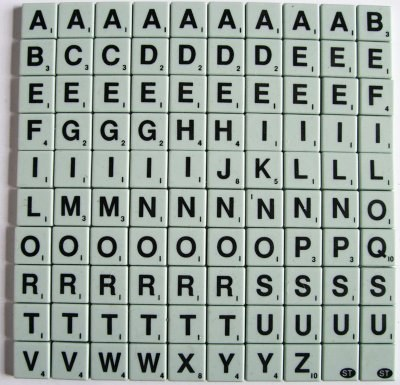
\includegraphics[width=\linewidth,height=4.6cm,keepaspectratio]{figs/photos/ch13_scrabble_en}
\caption{A full English Scrabble set: twelve E's, nine A's and I's, one each of J, K, Q, X and
Z---a letter-frequency table you can hold in your hand.\mdccredit{ch13_scrabble_en}}
\label{fig:ch13_scrabble_en}\end{minipage}
\end{figure}

The most famous application of entropy to a real source is Shannon's 1951 paper ``Prediction and
entropy of printed English''. With 26 letters and a space, a source that chose letters uniformly
would produce $\log_227=4.75$ bits per character. English is far from uniform: E, T, A, O and the
space are common, while Q, X, J and Z are rare. Accounting for single-letter frequencies alone
reduces the entropy to about 4.0 bits per character; accounting for pairs and triples of letters
(``th'', ``qu'', ``ing'') reduces it to about 3.3 and 3.1. Figure~\ref{fig:ch13_entropy}(b) shows
Shannon's staircase. We can repeat the measurement on a text you have in your hands: this book.
Figure~\ref{fig:ch13_letter_freq} counts the 2.4 million letters and spaces of its chapters.

\mdcfig{ch13_letter_freq}{Letter frequencies measured on the text of this book (all chapters,
with mathematics and \LaTeX\ commands stripped). The space is the most common symbol of all; E, T,
A, I, O and N (red) are the big six; Q, X, Z and J are vanishingly rare. Using these frequencies
alone, each character carries 4.12 bits rather than the 4.75 bits of a uniform 27-symbol source.}

The single-letter frequencies of a technical book are not quite those of Shannon's novels and
newspapers (``I'' and ``N'' are boosted by words such as \emph{information} and \emph{signal}),
but the conclusion is the same: frequency alone saves only about 13\%. The big savings come from
\emph{context}. Shannon made the point unforgettable in 1948 with a series of ``approximations to
English'': random text generated from letter frequencies, then from letter-pair statistics, then
from triples, then from word statistics. As the statistics improve, the gibberish begins to look
like language (Figure~\ref{fig:ch13_shannon_approx}). Large language models are this experiment
taken to its logical extreme.

\mdcfig{ch13_shannon_approx}{Shannon's approximations to English, regenerated from this book's own
text with a fixed random seed. Each line is drawn from a richer statistical model than the one
above it. By five-letter context, most ``words'' are real; with word-pair statistics, the output
reads like a communications engineer talking in their sleep.}

To go further Shannon used a human predictor. He showed subjects a passage one letter at a time
and asked them to guess the next letter, counting how many guesses each letter needed. Because a
fluent reader knows grammar, idiom and the thread of the argument, the guesses were often right
first time, and Shannon's bounds placed the entropy of long passages between roughly 0.6 and 1.3
bits per character. The \term{redundancy} of a source, $1-H/\log_2|\mathcal{X}|$, is therefore
around 75\% for English: three-quarters of the letters are, in an information-theoretic sense,
predictable from context. That redundancy is why you can read a text message with typos, why
crosswords are possible, and why good compressors shrink English text by factors of three to
five. Modern language models, which are nothing but very good next-token predictors, reach
cross-entropies on English text that are consistent with Shannon's range, and data compressors
built on them are among the best ever measured.

\mdcfig{ch13_compressors}{Bits per character of this book's text, estimated in two ways.
Navy: conditional entropies $F_N$ from the measured $N$-letter statistics (the estimates for
$N\ge4$ are biased low, because 2.4 million characters cannot populate all the longer contexts).
Green: the actual output of three everyday compressors run on the same text. Each better model
finds a lower number; none yet reaches the 0.6--1.3 bits of Shannon's human predictors (shaded).}

Figure~\ref{fig:ch13_compressors} completes the experiment. The general-purpose compressors on
your computer squeeze this book's text to about 2 to 2.6 bits per character: better than any
single-letter model, worse than a human reader. They are not broken. They simply use a weaker
model of English than you do.

\begin{tryit}[Measure the entropy of your own text]
Open Lab 19 (\lab{lab19\_information\_theory.py}) and choose the \emph{Entropy of text and images}
experiment. Paste in an e-mail, a page of code and a paragraph in another language. Watch the
letter histogram and the $F_0$--$F_3$ staircase, and compare them with the compressor bars. Which
text is the most predictable? Then set the source to \emph{Photograph} and switch the image
predictor from raw pixels to \emph{Left neighbour}: compare the entropy of the pixels with the
entropy of the differences between neighbouring pixels.
\end{tryit}

\begin{inpractice}[Morse code: entropy coding in 1838]
Long before Shannon, telegraph engineers practised variable-length coding. In the American Morse
code devised by Samuel Morse and Alfred Vail, and in the International Morse code that descends
from it (Figure~\ref{fig:ch13_morse}), the commonest letter, E, is a single dot and T a single
dash, while Q, Y and J need four symbols. The story goes that Vail estimated letter frequencies
by counting the pieces of type in a printer's type case. Short codes for frequent symbols is
exactly the principle that Huffman made optimal in 1951 and that every compressor uses today.
Morse's assignment is not optimal by Huffman's standards, but it captures most of the gain---not
bad for an age that had no word for entropy.
\end{inpractice}

\mdcphoto[0.27]{ch13_morse}{The International Morse code. Frequent letters (E, T, A, I, N)
get the shortest codes, an early form of entropy coding.}

\subsection{Sources with memory: Markov chains and entropy rate}

Real sources have memory: letters depend on previous letters, pixels on neighbouring pixels,
speech samples on previous samples. Knowing the past makes the next symbol less surprising, so the
information per symbol is lower than the single-symbol entropy suggests. For a stationary random
process $X_1,X_2,\ldots$ the relevant quantity is the \term{entropy rate}
\begin{equation}
\mathcal{H}(\mathcal{X})=\lim_{n\to\infty}\frac1nH(X_1,\ldots,X_n)
=\lim_{n\to\infty}H(X_n\mid X_{n-1},\ldots,X_1),
\label{eq:ch13:rate}
\end{equation}
where the two limits exist and are equal for any stationary process. The second form says the
entropy rate is the uncertainty about the next symbol given the entire past---exactly what
Shannon's guessing experiment measured. For a stationary \term{Markov source}, in which the next
state depends only on the current one through a transition matrix $P_{ij}=\Pr(X_{n+1}=j\mid
X_n=i)$ with stationary distribution $\pi$, the limit is reached immediately:
\begin{equation}
\mathcal{H}=H(X_2\mid X_1)=\sum_i\pi_i\,H(P_{i1},P_{i2},\ldots).
\label{eq:ch13:markov}
\end{equation}
In words: average, over the states you might be in, the uncertainty of the next step from that
state.

\begin{figure}[htbp]\centering
\begin{tikzpicture}[st/.style={circle,draw=navy,fill=navy!6,thick,minimum size=1.3cm,font=\sffamily\scriptsize,align=center},
  e/.style={-{Stealth[length=2mm]},thick,navy!70}]
\node[st] (a) at (0,0) {0\\quiet\\$\pi_0=0.75$};
\node[st,draw=accent,fill=accent!6] (b) at (4,0) {1\\busy\\$\pi_1=0.25$};
\draw[e] (a) to[bend left=25] node[above,font=\scriptsize]{0.1} (b);
\draw[e] (b) to[bend left=25] node[below,font=\scriptsize]{0.3} (a);
\draw[e] (a) to[loop left,looseness=6] node[left,font=\scriptsize]{0.9} (a);
\draw[e] (b) to[loop right,looseness=6] node[right,font=\scriptsize]{0.7} (b);
\node[font=\sffamily\scriptsize,align=left,anchor=west] at (6.4,0)
 {memoryless view: $h(0.25)=0.811$ bits\\with memory: $\mathcal{H}=0.572$ bits\\saving: 30\%};
\end{tikzpicture}
\caption{The two-state Markov sensor of the worked example. The long-run frequencies alone say
0.811 bits per report; knowing that the sensor tends to stay where it is cuts the true information
rate to 0.572 bits.}
\label{fig:ch13_markov}
\end{figure}

\begin{worked}[A two-state Markov source]
A binary sensor reports ``quiet'' (0) or ``busy'' (1) (Figure~\ref{fig:ch13_markov}). When quiet it
stays quiet with probability 0.9; when busy it stays busy with probability 0.7. The stationary
distribution solves $\pi_1=0.1\pi_0+0.7\pi_1$, giving $\pi_0=0.75$ and $\pi_1=0.25$. A memoryless
model that used only these long-run frequencies would assign $h(0.25)=0.811$ bits per report. The
entropy rate is
\[
\mathcal{H}=0.75\,h(0.1)+0.25\,h(0.3)=0.75(0.469)+0.25(0.881)=0.572\ \text{bits per report}.
\]
Exploiting the memory saves 30\% compared with coding each symbol independently---the principle
behind run-length coding of fax images, predictive coding of speech and the context modelling of
every modern compressor.
\end{worked}

Pictures have memory too, in two dimensions. Figure~\ref{fig:ch13_image_entropy} takes the
photograph of Bell Labs in Figure~\ref{fig:ch13_bell_labs}, converted to 8-bit grey levels. Coded
pixel by pixel, it needs 7.5 bits per pixel---nearly the full eight. But neighbouring pixels are
similar, so the \emph{difference} between a pixel and its left neighbour is usually small, and its
entropy is only 4.1 bits. Predict, then code the surprise: that two-line recipe is the heart of lossless image
compression in PNG and of the predictive coders of Chapter~\ref{ch:sourcecoding}.

\mdcfig{ch13_image_entropy}{Memory in a picture. Left: the histogram of grey levels in the Bell
Labs photograph is broad, so a memoryless code needs almost 8 bits per pixel. Right: the
difference between each pixel and its left-hand neighbour is sharply peaked at zero, and its
entropy is several bits lower. Prediction turns redundancy into savings.}

%======================================================================
\section{Mutual information and its algebra}
\label{sec:ch13:mi}
%======================================================================

Communication always involves at least two random variables: what was sent and what was received.
If the line is perfect, knowing one tells you everything about the other; if the line is dead,
knowing one tells you nothing. Real channels sit in between, and information theory needs a ruler
for ``how much does $Y$ tell me about $X$?''. Building that ruler takes three short steps.

\subsection{Joint and conditional entropy}

For a pair $(X,Y)$ with joint distribution $p(x,y)$, the \term{joint entropy}
\[
H(X,Y)=-\sum_{x,y}p(x,y)\log_2p(x,y)
\]
is just the entropy of the pair treated as one variable. The
\term{conditional entropy}
\begin{equation}
H(Y\mid X)=\sum_xp(x)H(Y\mid X=x)=-\sum_{x,y}p(x,y)\log_2p(y\mid x)
\label{eq:ch13:cond}
\end{equation}
is the average remaining uncertainty about $Y$ once $X$ is known. Because $p(x,y)=p(x)p(y\mid
x)$, taking logarithms and averaging gives the \term{chain rule}
\begin{equation}
H(X,Y)=H(X)+H(Y\mid X)=H(Y)+H(X\mid Y),
\label{eq:ch13:chain}
\end{equation}
and more generally $H(X_1,\ldots,X_n)=\sum_iH(X_i\mid X_{i-1},\ldots,X_1)$. In words: the
uncertainty of a pair is the uncertainty of the first plus that of the second \emph{given} the
first---the number of questions to identify both is the questions for the first, then the extra
questions for the second once you know the first. Conditioning never increases entropy on average,
$H(Y\mid X)\le H(Y)$, with equality if and only if $X$ and $Y$ are independent. (A particular
observation $X=x$ can increase uncertainty---a surprising test result can make you less
sure---but the average cannot.)

\subsection{Relative entropy: the cost of a wrong map}

Before defining mutual information we need a way to compare two probability distributions.

\begin{analogy}[The tourist's phrase book]
A tourist arrives with a phrase book written for a different dialect. The phrases still work,
but the ones she uses most often are long and clumsy, because the book's author expected them to
be rare. Every conversation costs her a little extra breath. Relative entropy is that extra
breath: the average number of additional bits you pay for coding a source with a code built for
the wrong statistics. Its limit: a real phrase book can be plain wrong, while a code built for
the wrong distribution still works perfectly---it is just longer than it needs to be.
\end{analogy}

The \term{relative entropy} or \term{Kullback--Leibler divergence} of $p$ from $q$ is
\begin{equation}
D(p\,\|\,q)=\sum_xp(x)\log_2\frac{p(x)}{q(x)}.
\label{eq:ch13:kl}
\end{equation}
Its operational meaning is exactly the tourist's penalty. A code designed for distribution $q$
uses about $\log_2(1/q(x))$ bits for symbol $x$; if the symbols actually follow $p$, the average
length is $H(p)+D(p\|q)$ instead of $H(p)$. Figure~\ref{fig:ch13_kl_mismatch} makes it concrete:
code our weather station with a code built for a place where snow is the commonest weather, and
every report costs 2.62 bits instead of 1.75---a penalty of exactly $D(p\|q)=0.88$ bits.

\mdcfig[0.5]{ch13_kl_mismatch}{The cost of a wrong map. The weather station of
Figure~\ref{fig:ch13_questions} (navy) coded with a code designed for a snowy climate (orange; the
numbers are codeword lengths). The code still works, but the average length grows from $H=1.75$ to
2.62 bits; the difference is the relative entropy.}

In hypothesis testing, $D(p\|q)$ is the exponential
rate at which the probability of mistaking $p$ for $q$ falls with the number of observations
(Stein's lemma). The single most useful inequality in information theory is
\begin{equation}
D(p\,\|\,q)\ge0,\qquad\text{with equality if and only if }p=q,
\label{eq:ch13:gibbs}
\end{equation}
known as \term{Gibbs' inequality}: you never \emph{save} by using the wrong map. The proof is one
line: since $\ln u\le u-1$, $-D(p\|q)\ln2=\sum p\ln(q/p)\le\sum p(q/p-1)=\sum q-\sum p\le0$.
Nearly every bound in this chapter---that entropy is maximised by the uniform distribution, that
conditioning reduces entropy, that mutual information is non-negative, that the Gaussian maximises
differential entropy---is~\eqref{eq:ch13:gibbs} in disguise. Note that $D$ is not symmetric and is
not a distance in the metric sense; it is nonetheless the natural measure of how distinguishable
two distributions are.

\subsection{Mutual information: the overlap of what two people know}

The \term{mutual information} between $X$ and $Y$ is the reduction in uncertainty about one
obtained by observing the other:
\begin{equation}
I(X;Y)=H(X)-H(X\mid Y)=H(Y)-H(Y\mid X)=H(X)+H(Y)-H(X,Y).
\label{eq:ch13:mi}
\end{equation}
Equivalently, it is the relative entropy between the joint distribution and the product of the
marginals,
\begin{equation}
I(X;Y)=D\big(p(x,y)\,\|\,p(x)p(y)\big)=\sum_{x,y}p(x,y)\log_2\frac{p(y\mid x)}{p(y)},
\label{eq:ch13:mikl}
\end{equation}
which shows at once that $I(X;Y)\ge0$, with equality exactly when $X$ and $Y$ are independent: it
measures how far the pair is from being unrelated. Mutual information is symmetric: $Y$ tells as
much about $X$ as $X$ tells about $Y$. For a communication channel with input $X$ and output $Y$,
$H(X)$ is what was sent, $H(X\mid Y)$ (the \term{equivocation}) is the uncertainty that remains
after reception, and their difference is what got through. Figure~\ref{fig:ch13_venn} shows the
relations as an area diagram.

\begin{figure}[htbp]\centering
\begin{tikzpicture}[scale=1.0]
\def\r{1.55}
\fill[navy!10] (0,0) circle (\r);
\fill[accent!10] (1.7,0) circle (\r);
\begin{scope}\clip (0,0) circle (\r); \fill[practc!22] (1.7,0) circle (\r); \end{scope}
\draw[navy,thick] (0,0) circle (\r);
\draw[accent,thick] (1.7,0) circle (\r);
\node[font=\sffamily\small,text=navy] at (-0.62,0) {$H(X\mid Y)$};
\node[font=\sffamily\small,text=accent] at (2.34,0) {$H(Y\mid X)$};
\node[font=\sffamily\small,text=practc!70!black,align=center] at (0.85,0) {$I(X;Y)$};
\node[font=\sffamily\small,text=navy] at (-0.9,1.62) {$H(X)$};
\node[font=\sffamily\small,text=accent] at (2.6,1.62) {$H(Y)$};
\draw[decorate,decoration={brace,amplitude=6pt,mirror},thick,gray] (-\r,-1.75) -- (1.7+\r,-1.75)
  node[midway,below=7pt,font=\sffamily\small,text=black] {$H(X,Y)$};
\node[font=\sffamily\scriptsize,text=navy,align=center] at (-3.1,-0.9) {what Alice sent\\but Bob still\\can't tell};
\node[font=\sffamily\scriptsize,text=accent,align=center] at (4.8,-0.9) {noise Bob\\received that\\says nothing\\about Alice};
\node[font=\sffamily\scriptsize,text=practc!70!black,align=center] at (0.85,2.25) {what got through};
\end{tikzpicture}
\caption{The information diagram for two random variables. Each circle is an entropy; the overlap
is the mutual information; the parts outside the overlap are the conditional entropies; and the
union is the joint entropy. For a channel, $H(X\mid Y)$ is the equivocation (what the receiver is
still unsure of) and $H(Y\mid X)$ is the entropy added by the noise.}
\label{fig:ch13_venn}
\end{figure}

\par\vspace{0pt plus 8\baselineskip}\penalty-300\vspace{0pt plus -8\baselineskip}
\begin{analogy}[Two witnesses]
Two people watched the same football match, one from the stands and one on a crackly radio. Each
``knows'' a certain amount about it---their entropies. Much of what they know is the same (the
score, who scored): that shared part is the mutual information. The radio listener also knows
things that are pure artefact of the crackle, and the spectator knows things the radio never
mentioned. A good channel is one where the overlap is almost all of what was sent. Like every
area picture, this one works for two people; Section~\ref{sec:ch13:mi}'s pitfall below shows how it
breaks for three.
\end{analogy}

The chain rule carries over: $I(X_1,\ldots,X_n;Y)=\sum_iI(X_i;Y\mid X_{i-1},\ldots,X_1)$, where the
\emph{conditional} mutual information $I(X;Y\mid Z)=H(X\mid Z)-H(X\mid Y,Z)$ is the information
$Y$ gives about $X$ when $Z$ is already known. This chain rule is the theoretical backbone of
multilevel coding, successive-interference cancellation and polar codes, all of which decompose a
hard channel into a sequence of easier ones, each conditioned on the decisions already made.

\begin{pitfall}[Three-circle diagrams lie]
It is tempting to extend Figure~\ref{fig:ch13_venn} to three variables with three overlapping
circles. The central region then represents $I(X;Y;Z)=I(X;Y)-I(X;Y\mid Z)$, which can be
\emph{negative}. The classic example: $X$ and $Y$ independent fair bits and $Z=X\oplus Y$. Any two
of the three are independent, so $I(X;Y)=0$, but given $Z$, $X$ determines $Y$, so
$I(X;Y\mid Z)=1$ and the ``area'' is $-1$ bit. Knowing the parity makes two independent bits
dependent---which is exactly how a parity check helps a decoder. Use the diagram for two
variables; for more, trust the algebra.
\end{pitfall}

\mdcfig[0.5]{ch13_dpi_chain}{Information about a BPSK symbol surviving each receiver stage at
$E_s/N_0=0$\,dB (mutual information computed by quadrature and Blahut--Arimoto, quantiser
thresholds optimised). Every quantiser loses something; the hard slicer loses 16\%.}

\subsection{The data-processing inequality}

\begin{analogy}[A photocopy of a photocopy]
Photocopy a page, then photocopy the copy, then copy that. Each generation is a little greyer
and fuzzier, and no amount of clever copying can make the tenth copy sharper than the first. You
can enlarge it, sharpen it, adjust the contrast; you cannot put back detail that was lost. The
limit of the analogy: some processing steps lose nothing at all, and the art of receiver design
is to find them.
\end{analogy}

\mdcfig{ch13_photocopy}{The data-processing inequality, photocopier edition (simulated: each copy
blurs slightly and adds a little noise). Every generation loses detail, and nothing done to a later
copy brings it back.}

Figure~\ref{fig:ch13_photocopy} runs the experiment. The mathematics says the same thing in one line.

If $X\to Y\to Z$ form a Markov chain---$Z$ depends on $X$ only through $Y$, as when $Z$ is any
processing of the received signal $Y$---then
\begin{equation}
I(X;Z)\le I(X;Y).
\label{eq:ch13:dpi}
\end{equation}
The proof uses the chain rule twice:
$I(X;Y,Z)=I(X;Z)+I(X;Y\mid Z)=I(X;Y)+I(X;Z\mid Y)$, and $I(X;Z\mid Y)=0$ by the Markov property,
so $I(X;Z)=I(X;Y)-I(X;Y\mid Z)\le I(X;Y)$. This is the \term{data-processing inequality}: no
processing of the received signal, however clever, can create information about what was sent.
Processing can only preserve it (when $Z$ is a \emph{sufficient statistic}, like the matched-filter
outputs of Chapter~\ref{ch:baseband}) or destroy it.

This inequality is a design tool. Every block in a receiver---filters, samplers, quantisers,
demappers, hard decisions---is a processing step, and each can only lose information. The matched
filter and symbol-rate sampler lose nothing (they produce a sufficient statistic); an ADC with too
few bits, a hard decision before the decoder, or a max-log approximation in the demapper all lose
something, and the loss can be measured in bits or, more usefully, in decibels.
Figure~\ref{fig:ch13_dpi_chain} measures it for the simplest receiver there is. At
$E_s/N_0=0$\,dB the soft matched-filter output carries 0.721 bits per BPSK symbol about the
transmitted bit. An 8-level (3-bit) quantiser keeps 0.714; a 4-level one keeps 0.693; a hard
decision keeps only 0.603. Notice how quickly the returns diminish: the first extra bit of ADC
resolution buys back most of the loss, and the third bit buys back almost all of it. That
diminishing return is why receiver designers can afford to be frugal with ADC bits in front of a
decoder, but not stingy.

\begin{inpractice}[Why soft decisions are worth 2\,dB]
Give a decoder only the sign of each matched-filter sample of BPSK and the channel becomes a
binary symmetric channel with crossover probability $\Q(\sqrt{2E_s/N_0})$. The data-processing
inequality guarantees a loss, and the capacity formulas of Section~\ref{sec:ch13:dmc} measure it.
At code rate $\frac12$ the minimum $E_b/N_0$ for reliable communication rises from 0.19\,dB (soft
decisions) to about 1.8\,dB (hard decisions); as the rate tends to zero the gap tends to
$10\log_{10}(\pi/2)=1.96$\,dB. Quantising each sample to three bits recovers all but about 0.2\,dB.
This is why every modern receiver passes \emph{log-likelihood ratios} (Chapter~\ref{ch:modulation})
rather than bits to the decoder, why deep-space receivers used 3-bit soft-decision Viterbi
decoders from the 1970s onwards, and why the 400G coherent-optics world migrated from
hard-decision to soft-decision FEC as soon as the DSP gates were affordable.
\end{inpractice}

\subsection{Fano's inequality}

How small can the error probability of a guess be, given how much uncertainty remains? Fano's
inequality answers with a number, and it is the hinge on which the ``you can't beat capacity''
half of Shannon's theorem turns. Suppose $\hat X$ is any estimate of $X$ formed from $Y$, with
error probability $P_e=\Pr(\hat X\ne X)$. \term{Fano's inequality} states
\begin{equation}
H(X\mid Y)\le h(P_e)+P_e\log_2\big(|\mathcal{X}|-1\big)\le1+P_e\log_2|\mathcal{X}|.
\label{eq:ch13:fano}
\end{equation}
The intuition is a two-step game of questions: to resolve the remaining uncertainty about $X$
given $Y$, first ask whether the estimate is right (at most $h(P_e)$ bits) and, if it is wrong,
ask which of the other $|\mathcal{X}|-1$ values is correct (at most $\log_2(|\mathcal{X}|-1)$ bits,
needed with probability $P_e$).

\mdcfig[0.5]{ch13_fano}{Fano's inequality read as a floor on error probability: the smallest
$P_e$ any receiver can achieve, given the equivocation $H(X\mid Y)$, for several alphabet sizes.}

Read backwards, Fano's inequality is a \emph{lower bound on error probability}: if the
equivocation $H(X\mid Y)$ is large, no receiver can have small $P_e$
(Figure~\ref{fig:ch13_fano}). If, after listening, you are still unsure by a full bit about which
of four messages was sent, then whatever you do you will be wrong at least about 19\% of the
time. The curves rise from zero: a small equivocation still allows a small error rate, but there
is no free lunch beyond the curve. In the converse of the channel coding theorem
(Section~\ref{sec:ch13:cct}), $X$ will be an entire message of $nR$ bits, and Fano's inequality
will tell us that if the channel cannot deliver enough mutual information to shrink the
equivocation, the error probability must stay bounded away from zero. That one line is why
capacity is a wall and not merely a guideline.

%======================================================================
\section{Typical sequences and the source coding theorem}
\label{sec:ch13:source}
%======================================================================

\subsection{The asymptotic equipartition property}

Here is a puzzle. Toss a biased coin with $\Pr(\text{heads})=0.1$ one thousand times. There are
$2^{1000}$ possible sequences, and the single most likely one is all tails. Yet you will
essentially never see it; its probability is $0.9^{1000}\approx10^{-46}$. What you will see is a
sequence with about 100 heads, and every such sequence has probability close to
\[
0.1^{100}\,0.9^{900}=2^{-1000\,[0.1\log_2(1/0.1)+0.9\log_2(1/0.9)]}=2^{-1000\,h(0.1)}=2^{-469}.
\]
How can the most likely sequence be one you never see? Because there is only \emph{one} all-tails
sequence, and there are an astronomical number of sequences with about a hundred heads. Each of
them is individually less likely, but together they hold almost all of the probability.
Figure~\ref{fig:ch13_coin_sequences} makes it visible: fourteen independent runs of 90 tosses look
different in detail and identical in character.

\mdcfig{ch13_coin_sequences}{Fourteen runs of 90 tosses of a coin that lands heads (red) 10\% of
the time. The individual patterns differ, but every run looks statistically the same: about nine
heads, scattered without obvious structure (the counts are on the right). The single most likely
sequence, all tails (grey bar), never appears. These are \emph{typical sequences}.}

\begin{analogy}[Every long novel looks the same to a statistician]
Pick two long English novels at random. Their plots have nothing in common, but count their
letters and you get almost exactly the same percentages of E, T and A. Long sequences generated by
the same source share their statistics, even though they share nothing else. The idea's limit:
it is a statement about \emph{long} sequences; a haiku and a telegram can be wildly atypical.
\end{analogy}

This is the \term{asymptotic equipartition property} (AEP): for a long sequence of independent,
identically distributed symbols,
\begin{equation}
-\frac1n\log_2p(X_1,\ldots,X_n)=\frac1n\sum_{i=1}^n\log_2\frac1{p(X_i)}\;\longrightarrow\;H(X)
\label{eq:ch13:aep}
\end{equation}
in probability. It is simply the law of large numbers applied to the random variable
$\log_2(1/p(X))$, whose mean is $H(X)$: the average surprise per symbol settles down to the
entropy. Figure~\ref{fig:ch13_aep}(a) shows the distribution of the left-hand side concentrating
around $H=0.469$ bits as $n$ grows.

\mdcfig{ch13_aep}{The asymptotic equipartition property for a binary source with $p=0.1$. (a) The
per-symbol ``sample entropy'' $-\frac1n\log_2p(X^n)$ concentrates around $H=0.469$ bits as the
sequence length $n$ grows. (b) Keep the most probable sequences and count them: the probability
captured jumps from near 0 to near 1 once about $2^{nH}$ sequences are kept---a vanishing fraction
of all $2^n$ sequences.}

The AEP splits the $|\mathcal{X}|^n$ possible sequences into two groups. The \term{typical set}
$A_\epsilon^{(n)}$ contains the sequences whose sample entropy is within $\epsilon$ of $H$. It has
three properties, each following from~\eqref{eq:ch13:aep}:
\begin{enumerate}
\item its total probability tends to one;
\item each member has probability between $2^{-n(H+\epsilon)}$ and $2^{-n(H-\epsilon)}$---all
typical sequences are roughly equally likely, hence ``equipartition'';
\item it contains between about $2^{n(H-\epsilon)}$ and $2^{n(H+\epsilon)}$ sequences.
\end{enumerate}
For the coin, the typical set holds about $2^{469}$ of the $2^{1000}$ sequences, a fraction of
$2^{-531}$, yet it holds nearly all the probability (Figure~\ref{fig:ch13_aep}(b)). The world of
long sequences is simple: nature picks, almost uniformly, one of about $2^{nH}$ typical sequences,
and everything else might as well not exist.

\begin{keyidea}[Entropy counts the sequences that matter]
$H$ has two faces. Seen from one symbol, it is an average surprise. Seen from a long block of $n$
symbols, it is a \emph{count}: there are about $2^{nH}$ sequences worth worrying about, each with
probability about $2^{-nH}$. Almost every theorem in this chapter---compression, channel coding,
sphere packing, rate--distortion---is proved by counting typical sequences.
\end{keyidea}

\subsection{The source coding theorem}

The AEP immediately suggests a compression scheme: number the typical sequences with
$\lceil n(H+\epsilon)\rceil$-bit indices, send the index, and use an escape flag followed by the
raw sequence for the rare atypical ones. The average length per symbol tends to
$H+\epsilon$, and $\epsilon$ can be made as small as we like. Conversely, any scheme using fewer
than $n(H-\epsilon)$ bits can index only a vanishing fraction of the typical set and so must fail
with probability tending to one. This is Shannon's \term{source coding theorem}: \emph{a
memoryless source with entropy $H$ can be compressed losslessly to $H$ bits per symbol, and no
further.} For sources with memory, $H$ is replaced by the entropy rate~\eqref{eq:ch13:rate}.

Think of the typical set as a telephone directory. You do not need to transmit the sequence
itself; you only need to say which page and line of the directory it is on, and the directory has
only $2^{nH}$ entries. That is the whole of lossless compression in one sentence.

\mdcfig{ch13_source_cliff}{The source coding theorem as a cliff. Index the $2^{nR}$ most probable
sequences of a biased coin ($p=0.1$) and count how often the sequence that actually occurs is
missing from the list. For long blocks the failure probability drops from one to essentially zero
as $R$ crosses $H=0.469$ bits.}

Figure~\ref{fig:ch13_source_cliff} shows the theorem at work. Allow fewer than $H$ bits per symbol
and the directory misses almost every sequence; allow a little more and it misses almost none, and
the longer the block the sharper the edge.

\subsection{Prefix codes and the Kraft inequality}

Block coding of typical sequences is a proof technique. Practical lossless compression uses
variable-length codes, and the theorem has a sharp, finite form for them. A code is a
\term{prefix code} (or instantaneous code) if no codeword is the beginning of another, so that the
decoder can recognise the end of each codeword as soon as it arrives---the weather code of
Figure~\ref{fig:ch13_questions} is one. The codeword lengths $\ell_1,\ell_2,\ldots$ of any binary
prefix code satisfy the \term{Kraft inequality}
\begin{equation}
\sum_i2^{-\ell_i}\le1,
\label{eq:ch13:kraft}
\end{equation}
and conversely any set of lengths satisfying it can be realised by a prefix code.

\mdcfig{ch13_kraft}{The Kraft inequality as a budget. A codeword of length $\ell$ claims a share
$2^{-\ell}$ of the unit interval (equivalently, of the leaves of a binary tree), and the shares of
a prefix code cannot overlap. Both the weather code and the Huffman code of
Figure~\ref{fig:ch13_huffman} spend the budget exactly; lengths 1, 1 and 2 would need 1.25 units,
so no prefix code with those lengths exists.}

Picture it as a budget (Figure~\ref{fig:ch13_kraft}): a codeword of length $\ell$ claims a
fraction $2^{-\ell}$ of the leaves at the bottom of a binary tree, and the subtrees of a prefix
code cannot overlap, so the claims cannot add up to more than one. Short codewords are expensive;
you can afford only a few. McMillan showed in 1956 that the same inequality holds for every
uniquely decodable code, prefix or not, so nothing is lost by insisting on the prefix property.

Minimising the average length $\bar L=\sum p_i\ell_i$ subject to~\eqref{eq:ch13:kraft} is a small
optimisation problem whose answer is the intuitive one: give each symbol a length equal to its
surprise, $\ell_i\approx\log_2(1/p_i)$. Rounding up to whole bits costs less than one bit, so
\begin{equation}
H(X)\le\bar L_{\text{opt}}<H(X)+1.
\label{eq:ch13:lbound}
\end{equation}
Coding blocks of $n$ symbols divides the one-bit overhead by $n$, so the average per symbol
approaches $H$.

\begin{deeper}[Proving the bounds on $\bar L$]
Ignoring the integer constraint, minimise $\sum p_i\ell_i$ subject to $\sum2^{-\ell_i}=1$ with a
Lagrange multiplier: the stationary point is $\ell_i=\log_2(1/p_i)$ and $\bar L=H$. With integer
lengths, the choice $\ell_i=\lceil\log_2(1/p_i)\rceil$ satisfies Kraft (since
$2^{-\ell_i}\le p_i$) and has $\ell_i<\log_2(1/p_i)+1$, which gives the upper bound. The lower
bound is Gibbs' inequality again: with $q_i=2^{-\ell_i}/\sum_j2^{-\ell_j}$,
\[
\bar L-H=\sum p_i\log_2\frac{p_i}{2^{-\ell_i}}=D(p\|q)+\log_2\frac1{\sum_j2^{-\ell_j}}\ge0,
\]
because both terms are non-negative (the second by Kraft). Equality requires $p_i=2^{-\ell_i}$:
every probability a power of two, as in the weather station.
\end{deeper}

\subsection{Huffman coding}

\begin{history}[A term paper that beat the professor]
In 1951 Robert Fano gave the students of his information theory course at MIT a choice: sit the
final examination, or write a term paper on finding the most efficient binary code. Fano and
Shannon had each proposed good methods (\emph{Shannon--Fano coding}, which splits the symbol list
top-down into halves of nearly equal probability), but neither had proved one optimal. David
Huffman, as he later told the story, worked on the problem for months, was on the point of giving
up and starting to revise for the exam, and then saw the answer: build the tree from the
\emph{bottom} up, starting with the two least probable symbols. The method was provably optimal and
simpler than anything his professor had found. Huffman published it in 1952 as ``A method for the
construction of minimum-redundancy codes''; it has been in daily use ever since.
\end{history}

\mdcphoto[0.28]{ch13_fano_photo}{Robert Fano (1917--2016) at MIT, whose class assignment
produced Huffman coding and whose inequality underpins the converse to Shannon's theorem.}

The optimal prefix code for a known distribution is found by Huffman's greedy algorithm:
repeatedly merge the two least probable symbols into a single node whose probability is their sum,
until one node remains; then read the codewords off the resulting tree. Why does it work? The two
rarest symbols must have the longest codewords in any optimal code, and they can always be made
siblings at the deepest level; merging them reduces the problem to a smaller one of exactly the
same kind. Figure~\ref{fig:ch13_huffman} works an example. Huffman coding is optimal among
symbol-by-symbol codes, and within one bit of the entropy by~\eqref{eq:ch13:lbound}; for the
five-symbol source of the figure it comes within 0.08\,bit. The algorithm runs in the time it takes
to sort the probabilities, which is why it fits comfortably inside a fax machine or a camera.

\begin{figure}[htbp]\centering
\begin{tikzpicture}[
  leaf/.style={draw=navy,fill=navy!6,thick,rounded corners=2pt,minimum width=1.25cm,minimum height=0.6cm,font=\sffamily\scriptsize,align=center},
  int/.style={draw=accent,fill=accent!6,thick,circle,inner sep=1pt,minimum size=0.7cm,font=\sffamily\scriptsize},
  e/.style={thick,navy!70},
  lab/.style={font=\sffamily\scriptsize\bfseries,text=accent}]
\node[leaf] (a) at (0,0) {a\;0.4\\\texttt{00}};
\node[leaf] (b) at (1.6,0) {b\;0.2\\\texttt{01}};
\node[leaf] (c) at (3.4,0) {c\;0.2\\\texttt{10}};
\node[leaf] (d) at (5.0,-1.2) {d\;0.1\\\texttt{110}};
\node[leaf] (ee) at (6.6,-1.2) {e\;0.1\\\texttt{111}};
\node[int] (de) at (5.8,0.2) {0.2};
\node[int] (cde) at (4.6,1.3) {0.4};
\node[int] (ab) at (0.8,1.3) {0.6};
\node[int] (root) at (2.7,2.4) {1.0};
\draw[e] (root) -- node[lab,above left]{0} (ab);
\draw[e] (root) -- node[lab,above right]{1} (cde);
\draw[e] (ab) -- node[lab,left]{0} (a);
\draw[e] (ab) -- node[lab,right]{1} (b);
\draw[e] (cde) -- node[lab,left]{0} (c);
\draw[e] (cde) -- node[lab,right]{1} (de);
\draw[e] (de) -- node[lab,left]{0} (d);
\draw[e] (de) -- node[lab,right]{1} (ee);
\node[font=\sffamily\scriptsize,align=left,anchor=west] at (7.6,1.0)
 {merge order:\\1.\;d+e $\to$ 0.2\\2.\;c+(de) $\to$ 0.4\\3.\;a+b $\to$ 0.6\\4.\;root};
\end{tikzpicture}
\caption{A Huffman code for five symbols with probabilities 0.4, 0.2, 0.2, 0.1 and 0.1. The two
least probable nodes are merged at each step (ties may be broken either way; this choice gives the
minimum-variance code). Average length 2.2\,bits, entropy 2.122\,bits, so the code is within
0.08\,bit of the bound~\eqref{eq:ch13:lbound}.}
\label{fig:ch13_huffman}
\end{figure}

\begin{inpractice}[Entropy coders in your pocket]
Huffman codes are in JPEG, MP3, the DEFLATE format inside every ZIP file and PNG image, and fax
machines. Their weakness is the integer codeword length: a symbol with probability 0.99 still
costs a whole bit, when its self-information is 0.0145 bits. \emph{Arithmetic coding}, which
codes an entire message as a single number in $[0,1)$---in effect, Figure~\ref{fig:ch13_kraft}'s
unit interval, subdivided again and again---removes this overhead and adapts easily to changing
statistics; it is the entropy coder in the main profiles of H.264 (CABAC) and in HEVC and AV1
video. The \emph{Lempel--Ziv} family (1977--78), which learns a dictionary of repeated strings on
the fly, is \emph{universal}: it approaches the entropy rate of any stationary ergodic source
without knowing its statistics. It is the ``zlib'' bar of Figure~\ref{fig:ch13_compressors}. The
practice of source coding for voice, audio, images and video is the subject of
Chapter~\ref{ch:sourcecoding}.
\end{inpractice}

\begin{tryit}[Build a Huffman code]
In Lab 19's \emph{Huffman coding} experiment, drag the probability sliders of a five-symbol source
and watch the tree rebuild itself. Make one symbol dominate (probability 0.9) and see the gap
between the average length and the entropy grow towards a full bit; then switch on coding of
\emph{pairs} of symbols and watch most of the gap close.
\end{tryit}

\begin{pitfall}[Entropy is a property of a model, not of a file]
``What is the entropy of this file?'' has no answer until you say which probabilistic model
generated it. A file of a million digits of $\pi$ looks like a memoryless uniform source with
$\log_210=3.32$ bits per digit, and a general-purpose compressor will get no closer than that; yet
a program of a few hundred bytes can generate it. Compressors estimate entropy under their own
model class, and a better model (context mixing, a language model) always finds a lower number,
as Figure~\ref{fig:ch13_compressors} showed. The deep version of this observation is Kolmogorov
complexity, the length of the shortest program that outputs the data, which is uncomputable. For
engineering, the lesson is modest: measured compression ratios are upper bounds on the entropy
rate, and ``random-looking'' is not the same as random. Encrypted or already-compressed data is
the one reliably incompressible input.
\end{pitfall}

\par\vspace{0pt plus 10\baselineskip}\penalty-300\vspace{0pt plus -10\baselineskip}
%======================================================================
\section{Discrete memoryless channels and their capacity}
\label{sec:ch13:dmc}
%======================================================================

\subsection{The channel as a conditional distribution}

From now on we stop asking how to describe a source and start asking how much a channel can
carry. Shannon's trick is to describe any channel, however complicated its physics, by one table:
for each input, the probabilities of each output. A \term{discrete memoryless channel} (DMC) has a
finite input alphabet $\mathcal{X}$, a finite output alphabet $\mathcal{Y}$ and a transition
probability $W(y\mid x)$; ``memoryless'' means that each use of the channel acts independently, so
that for blocks of $n$ uses $W(y^n\mid x^n)=\prod_iW(y_i\mid x_i)$. The DMC is an abstraction, but a
useful one: a modulator, a physical channel and a demodulator with a finite set of outputs together
form a DMC, and the information theorist's job is to say how many bits per use it can carry.
Figure~\ref{fig:ch13_channels} shows the three most important binary examples.

\begin{figure}[htbp]\centering
\begin{tikzpicture}[x=1cm,y=1cm,
  dot/.style={circle,fill=navy,inner sep=1.6pt},
  lb/.style={font=\sffamily\scriptsize},
  a/.style={-{Stealth[length=1.8mm]},thick,navy},
  b/.style={-{Stealth[length=1.8mm]},thick,accent,dashed}]
% BSC
\begin{scope}
\node[font=\sffamily\small\bfseries,text=navy] at (1.2,1.9) {BSC};
\node[dot,label=left:{\small 0}] (x0) at (0,1) {}; \node[dot,label=left:{\small 1}] (x1) at (0,0) {};
\node[dot,label=right:{\small 0}] (y0) at (2.4,1) {}; \node[dot,label=right:{\small 1}] (y1) at (2.4,0) {};
\draw[a] (x0) -- node[lb,above]{$1-p$} (y0); \draw[a] (x1) -- node[lb,below]{$1-p$} (y1);
\draw[b] (x0) -- node[lb,pos=0.28,above,sloped]{$p$} (y1); \draw[b] (x1) -- node[lb,pos=0.28,below,sloped]{$p$} (y0);
\end{scope}
% BEC
\begin{scope}[xshift=4.6cm]
\node[font=\sffamily\small\bfseries,text=navy] at (1.2,1.9) {BEC};
\node[dot,label=left:{\small 0}] (x0) at (0,1) {}; \node[dot,label=left:{\small 1}] (x1) at (0,0) {};
\node[dot,label=right:{\small 0}] (y0) at (2.4,1.2) {}; \node[dot,label=right:{\small ?}] (ye) at (2.4,0.5) {};
\node[dot,label=right:{\small 1}] (y1) at (2.4,-0.2) {};
\draw[a] (x0) -- node[lb,above]{$1-p$} (y0); \draw[a] (x1) -- node[lb,below]{$1-p$} (y1);
\draw[b] (x0) -- node[lb,pos=0.6,above]{$p$} (ye); \draw[b] (x1) -- node[lb,pos=0.6,below]{$p$} (ye);
\end{scope}
% Z
\begin{scope}[xshift=9.2cm]
\node[font=\sffamily\small\bfseries,text=navy] at (1.2,1.9) {Z-channel};
\node[dot,label=left:{\small 0}] (x0) at (0,1) {}; \node[dot,label=left:{\small 1}] (x1) at (0,0) {};
\node[dot,label=right:{\small 0}] (y0) at (2.4,1) {}; \node[dot,label=right:{\small 1}] (y1) at (2.4,0) {};
\draw[a] (x0) -- node[lb,above]{$1$} (y0); \draw[a] (x1) -- node[lb,below]{$1-p$} (y1);
\draw[b] (x1) -- node[lb,pos=0.3,below,sloped]{$p$} (y0);
\end{scope}
\end{tikzpicture}
\caption{Three binary channels. The binary symmetric channel (BSC) flips each bit with probability
$p$: a hard-decision demodulator in Gaussian noise. The binary erasure channel (BEC) either
delivers the bit or announces that it was lost: a packet network with checksums, or a receiver
that flags unreliable symbols. The Z-channel never corrupts a zero but loses a one with
probability $p$: an optical on--off link in which a pulse can fail to register but darkness
cannot produce one, or a memory cell that can leak charge but not gain it.}
\label{fig:ch13_channels}
\end{figure}


\subsection{Capacity: a speed limit no clever driving can beat}

For a given input distribution $p(x)$, the channel induces a joint distribution
$p(x)W(y\mid x)$ and hence a mutual information $I(X;Y)$. The input distribution is the designer's
to choose, the channel is not, so Shannon defined the \term{capacity} of the channel as
\begin{equation}
C=\max_{p(x)}I(X;Y)\quad\text{bits per channel use}.
\label{eq:ch13:capacity}
\end{equation}
In words: try every way of using the inputs, and keep the one that gets the most information
through. At this point the definition is just a number computed from $W$. Its meaning comes from
the channel coding theorem of the next section: $C$ is the highest rate at which information can
be sent with arbitrarily small error probability.

\begin{analogy}[The highway speed limit]
Think of capacity as a speed limit set by physics rather than by the police. Below it, a skilled
driver (a good code) can go as fast as she likes in perfect safety, provided she plans far enough
ahead (a long block). Above it, no driver, car or route gets through: crashes are guaranteed. The
analogy's limit is a happy one: on a real highway, driving just under the limit is still risky,
but on Shannon's highway the risk can be made as small as you please. You pay for that safety in
planning distance, which is delay.
\end{analogy}

Now compute capacity for the channels of Figure~\ref{fig:ch13_channels}.

\paragraph{Binary symmetric channel.} Whatever the input distribution,
$H(Y\mid X)=h(p)$, because given the input the output is a coin flip with bias $p$. So
$I(X;Y)=H(Y)-h(p)\le1-h(p)$, with equality when $Y$ is uniform, which a uniform input achieves:
\begin{equation}
C_{\text{BSC}}=1-h(p).
\label{eq:ch13:bsc}
\end{equation}
Read it as ``one bit per use, minus the uncertainty the noise adds''. A BSC with $p=0.11$ has
capacity 0.5: it can carry one information bit for every two channel bits, reliably, despite
corrupting 11\% of them. At $p=\frac12$ the output is independent of the input and $C=0$; at $p=1$
the channel is perfect (just invert every bit).

\begin{figure}[H]\centering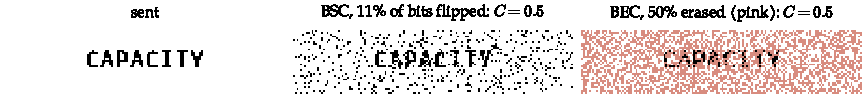
\includegraphics[width=0.92\linewidth]{figs/ch13_channel_pictures}\caption{Two channels with the same capacity of half a bit per use. A bitmap
sent through a BSC that flips 11\% of its pixels, and through a BEC that erases half of them (pink).
The erasure channel looks far worse, yet it carries exactly as much information: the receiver knows
\emph{which} pixels are missing, while the BSC hides its errors among the good pixels.}\label{fig:ch13_channel_pictures}\end{figure}

Figure~\ref{fig:ch13_channel_pictures} compares the BSC with the next channel at equal capacity.
The eye is a poor judge of information: half the picture gone looks far worse than a light
sprinkle of flipped pixels, but knowing where the damage is turns out to be worth exactly as much
as having fewer, hidden errors.

\paragraph{Binary erasure channel.} With input $\Pr(X=1)=q$,
$H(X\mid Y)=p\,h(q)$---uncertainty remains only when an erasure occurs---so
$I(X;Y)=h(q)-p\,h(q)=(1-p)h(q)$ and
\begin{equation}
C_{\text{BEC}}=1-p.
\label{eq:ch13:bec}
\end{equation}
The result is intuitive: a fraction $p$ of the bits are lost and the receiver knows which, so
at most a fraction $1-p$ can carry information. What is not intuitive is that this rate is
\emph{achievable} without feedback: the transmitter does not know which bits will be erased, yet
a good code lets the receiver recover the message from any $\approx n(1-p)$ unerased positions.
Fountain codes (LT and Raptor codes), used for broadcast file delivery in 3GPP MBMS and DVB, come
close to this in practice; Reed--Solomon codes achieve it exactly for erasures within a block
(Chapter~\ref{ch:classiccodes}).

\paragraph{Z-channel.} Here symmetry fails and the optimum input is not uniform. With
$\Pr(X=1)=q$, the output is 1 with probability $q(1-p)$, and
$I(X;Y)=h\big(q(1-p)\big)-q\,h(p)$. Setting the derivative to zero gives
\begin{equation}
C_{\text{Z}}=\log_2\!\big(1+(1-p)\,p^{p/(1-p)}\big),
\label{eq:ch13:z}
\end{equation}
achieved with $q<\frac12$: send fewer ones, because ones are the unreliable symbol. At $p=\frac12$,
$C=\log_21.25=0.322$ bits with $q=0.4$. Figure~\ref{fig:ch13_dmc_capacity} compares the three
capacities and shows the mutual information as a function of the input distribution. Two
general facts are visible: mutual information is a \emph{concave} function of $p(x)$, so it has a
single maximum and no local traps; and for channels with enough symmetry (the BSC, the BEC, and
any channel whose transition matrix has rows and columns that are permutations of each other) the
uniform input is optimal.

\begin{figure}[H]\centering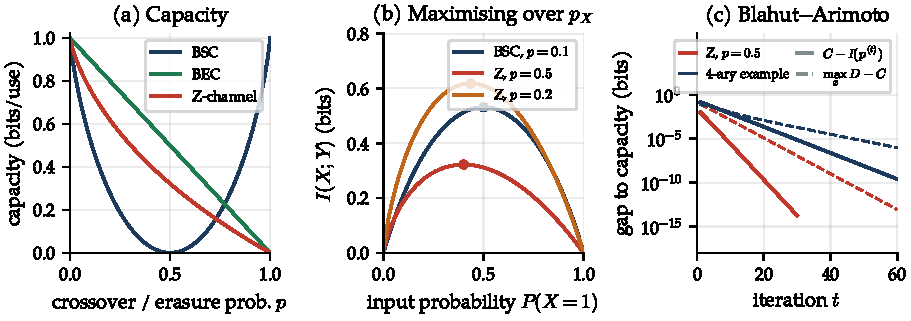
\includegraphics[width=0.92\linewidth]{figs/ch13_dmc_capacity}\caption{(a) Capacities of the BSC, BEC and Z-channel as a function of the
crossover or erasure probability. (b) Mutual information versus input distribution. For the
symmetric BSC the maximum is at $P(X=1)=\frac12$; for the Z-channel it moves towards the reliable
symbol. (c) Convergence of the Blahut--Arimoto algorithm for the Z-channel with $p=0.5$ and for a
four-input channel in which one input is useless: the gap between capacity and the lower bound
$I(p^{(t)})$ (solid) and the upper bound $\max_xD(W(\cdot|x)\|q^{(t)})$ (dashed).}\label{fig:ch13_dmc_capacity}\end{figure}

\subsection{Computing capacity: the Blahut--Arimoto algorithm}

For a general DMC the maximisation~\eqref{eq:ch13:capacity} has no closed form, but because it is
concave it can be solved numerically, and in 1972 Richard Blahut and Suguru Arimoto independently
found an elegant iterative algorithm. The idea is a kind of natural selection among input
letters. Start with any input distribution $p^{(0)}(x)>0$. At iteration $t$, compute the output
distribution $q^{(t)}(y)=\sum_xp^{(t)}(x)W(y\mid x)$ and, for each input letter, the divergence
$D_x=D\big(W(\cdot\mid x)\,\|\,q^{(t)}\big)$---how distinguishable that input's output distribution
is from the average. Then update
\begin{equation}
p^{(t+1)}(x)=\frac{p^{(t)}(x)\,2^{D_x}}{\sum_{x'}p^{(t)}(x')\,2^{D_{x'}}}.
\label{eq:ch13:ba}
\end{equation}
Inputs that stand out from the crowd get more probability; inputs that blend in get less. Figure~\ref{fig:ch13_ba_evolution} watches the selection happen. At every
step $\sum_xp^{(t)}(x)D_x=I(p^{(t)})\le C\le\max_xD_x$, so the gap between the two bounds is a
certificate of how close the answer is (Figure~\ref{fig:ch13_dmc_capacity}(c)). At the optimum
every input that is used has the same divergence $D_x=C$, and unused inputs have $D_x\le C$---a
beautiful characterisation: in a capacity-achieving code, every input letter in use is equally
informative. The same alternating structure computes rate--distortion functions
(Section~\ref{sec:ch13:rd}) and is a cousin of the expectation--maximisation algorithms of
statistics and machine learning.

\begin{figure}[htbp]\centering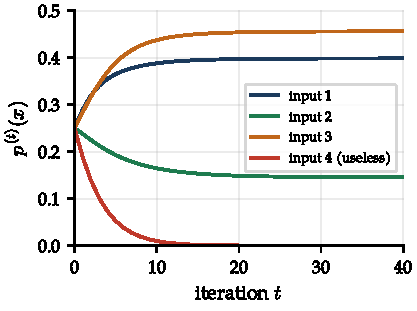
\includegraphics[width=0.45\linewidth]{figs/ch13_ba_evolution}\caption{Blahut--Arimoto as natural selection, for the four-input channel of
Figure~\ref{fig:ch13_dmc_capacity}(c). Starting from a uniform input, the useless fourth input (red),
whose outputs look like everyone else's, is starved of probability, while the distinctive inputs
settle at their optimal shares within a few dozen iterations.}\label{fig:ch13_ba_evolution}\end{figure}

\begin{worked}[The capacity of hard-decision BPSK]
A BPSK link at $E_s/N_0=0$\,dB is followed by a hard-decision slicer. The crossover probability is
$p=\Q(\sqrt{2E_s/N_0})=\Q(1.414)=0.0786$, so the resulting BSC has capacity
$1-h(0.0786)=1-0.397=0.603$ bits per channel use. Had the decoder been given the soft
matched-filter outputs instead, the capacity of the binary-input Gaussian channel at the same SNR
(computed in Section~\ref{sec:ch13:constrained}) would be 0.72 bits. The slicer throws away about
16\% of the capacity (the bottom bar of Figure~\ref{fig:ch13_dpi_chain}); equivalently, to support
rate $\frac12$ it needs about 1.6\,dB more signal energy---the data-processing loss of the
In-Practice box in Section~\ref{sec:ch13:mi}.
\end{worked}

\begin{tryit}[Capacity of any channel you can draw]
Lab 19's \emph{DMC capacity} experiment runs Blahut--Arimoto on a transition matrix you edit.
Start from a BSC and drag $p$ from 0 to 0.5: watch the optimal input stay uniform while the
capacity falls along $1-h(p)$. Switch to the Z-channel and watch the optimal $P(X=1)$ slide below
one half. Then switch on \emph{Add a useless input X = u}, an extra input row equal to the average
of the others, and see the
algorithm starve it of probability.
\end{tryit}

\begin{figure}[htbp]\centering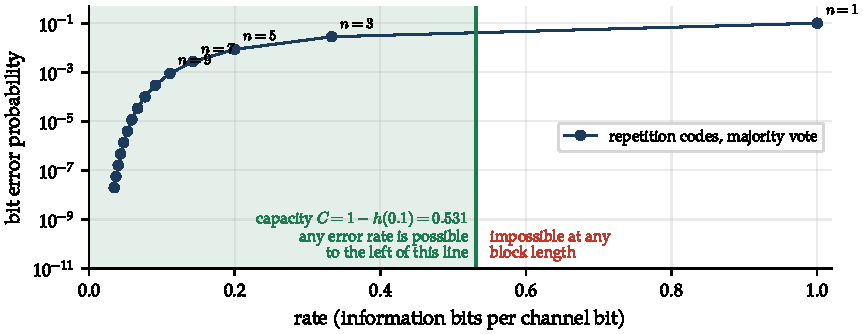
\includegraphics[width=0.85\linewidth]{figs/ch13_repetition}\caption{The pre-1948 view and Shannon's. On a BSC with $p=0.1$, repetition codes
(navy) buy reliability only by giving up rate: to reach $10^{-8}$ they need about 30 repetitions and
a rate near 0.03. Shannon's theorem says the whole green region is reachable: any error rate at
any rate below $C=0.531$, given long enough blocks. To the right of the line, nothing works.}\label{fig:ch13_repetition}\end{figure}

\par\vspace{0pt plus 10\baselineskip}\penalty-300\vspace{0pt plus -10\baselineskip}
%======================================================================
\section{The channel coding theorem}
\label{sec:ch13:cct}
%======================================================================

\subsection{Codes, rates and error probability}

An $(M,n)$ \term{block code} for a channel maps each of $M$ messages $w\in\{1,\ldots,M\}$ to a
codeword $x^n(w)$ of $n$ channel symbols; the decoder maps each received sequence $y^n$ back to an
estimate $\hat w$. The \term{code rate} is $R=\log_2M/n$ bits per channel use. A rate $R$ is
\emph{achievable} if there is a sequence of $(2^{nR},n)$ codes whose maximum error probability over
all messages tends to zero as $n\to\infty$.

\begin{keyidea}[The noisy channel coding theorem]
Every discrete memoryless channel has a capacity $C=\max_{p(x)}I(X;Y)$ such that
\begin{itemize}
\item \emph{(achievability)} every rate $R<C$ is achievable: for any $\epsilon>0$ and all
sufficiently large $n$ there exist codes of rate $R$ with error probability below $\epsilon$;
\item \emph{(converse)} no rate $R>C$ is achievable: for such rates the error probability is
bounded away from zero, and in fact tends to one.
\end{itemize}
Noise does not limit reliability; it limits rate. Below capacity, reliability is a matter of
block length and decoder complexity, not of physics.
\end{keyidea}

\mdcfig{ch13_noise_clouds}{The counting argument in two dimensions. Each cross is a codeword; the
dots are where the noise carries it. With few codewords (left) the clouds are separate and the
receiver can tell them apart; with too many (right) they overlap and errors are unavoidable.
Capacity is the largest number of clouds that fit, per dimension, as the dimension grows.}

It is hard to overstate how strange this sounded in 1948. Engineers generally assumed the
opposite: that to reduce the error rate you had to slow down, repeating each bit more and more
times, so that perfect reliability required zero rate. The repetition code on a BSC with $p=0.1$
illustrates the belief: three repetitions and a majority vote reduce the error rate to 0.028 at
rate $\frac13$; five give 0.0086 at rate $\frac15$; the error rate falls only as the rate falls
(Figure~\ref{fig:ch13_repetition}). Shannon's theorem says that the same channel can carry 0.531
bits per use with error probability as small as you like. The difference between the repetition
code and a good code is that the good code spreads each information bit across \emph{many} channel
symbols in a way that lets the noise average out.

\subsection{Why mutual information? A counting argument}

The AEP makes the theorem plausible with a few lines of counting. Send a codeword $x^n$ of a code
whose symbols look like draws from $p(x)$. The received $y^n$ is, with high probability, one of
about $2^{nH(Y\mid X)}$ sequences typical for that input: the noise ``fans out'' each codeword
into a cloud of that size. All received sequences, taken over all codewords, are typical for the
output distribution, of which there are about $2^{nH(Y)}$. If the clouds belonging to different
codewords are to be told apart they must not overlap much, so the number of codewords is at most
\begin{equation}
M\lesssim\frac{2^{nH(Y)}}{2^{nH(Y\mid X)}}=2^{n[H(Y)-H(Y\mid X)]}=2^{nI(X;Y)},
\label{eq:ch13:count}
\end{equation}
and the rate is at most $I(X;Y)$. Choosing the best input distribution gives $C$. In words:
capacity is the number of non-overlapping noise clouds you can fit into the space of things the
receiver might see. Figure~\ref{fig:ch13_noise_clouds} draws the idea.


For the BSC the picture is geometric. Each codeword's cloud is a \emph{Hamming sphere}: the
roughly $\binom{n}{np}\approx2^{nh(p)}$ binary sequences within Hamming distance $np$ of it. The whole
space holds $2^n$ sequences, so at most $2^{n(1-h(p))}$ non-overlapping spheres fit, which is
$C_{\text{BSC}}$ again. The channel coding problem is a \term{sphere-packing} problem, and much of
the history of coding theory is the history of trying to pack spheres well in spaces of very high
dimension.

\mdcfig[0.5]{ch13_random_distances}{Darts in many dimensions. The distance between two random
points on a unit sphere, for several dimensions $n$. In two dimensions random darts can land
anywhere, even on top of each other; in a thousand dimensions they are almost always at the same,
large distance. Random codebooks are good codebooks.}

\subsection{Random coding: Shannon's existence proof}

The counting argument shows that $I(X;Y)$ is an upper limit. The astonishing part of Shannon's
theorem is that it can be reached, and his proof of this is one of the great ideas of
twentieth-century mathematics. Rather than construct a good code, he \emph{averaged over all
codes}.

\begin{analogy}[Throwing darts in the dark]
Suppose you must place a few thousand dots on a huge dartboard so that no two are close. You
could spend a lifetime designing a pattern. Or you could throw darts blindfolded. In two
dimensions random darts clump badly; but in a space of a thousand dimensions there is so much room
that random darts land, almost always, far from each other. Shannon's proof is the observation that
blindfolded dart-throwing works in high dimensions. The catch, which took fifty years to get
around, is that a random pattern is hard to \emph{read}: to find the dart nearest a received
point, you must check them all.
\end{analogy}

Figure~\ref{fig:ch13_random_distances} shows the dartboard effect with real numbers: draw pairs of
random points on a sphere and measure their distance. In two dimensions the distances are spread
from zero upwards; in a thousand they cluster tightly around the same large value, and a
dangerously close pair essentially never occurs.

Generate a codebook at random: each of the $2^{nR}$ codewords is a sequence of $n$ independent
symbols drawn from $p(x)$. Reveal the codebook to both ends. To decode, the receiver looks for the
unique codeword that is \term{jointly typical} with what it received---one whose pairing with
$y^n$ has the statistics expected of an input--output pair. An error happens in only two ways: the
right codeword does not look typical (rare, by the AEP), or a wrong codeword happens to look
typical by accident. A wrong codeword was drawn independently of $y^n$, and each has only about a
$2^{-nI(X;Y)}$ chance of fooling the receiver; with $2^{nR}$ of them, the total risk is about
$2^{-n(I(X;Y)-R)}$, which vanishes whenever $R<I(X;Y)$. So the error probability \emph{averaged
over the random choice of codebook} tends to zero---and if the average is small, at least one
codebook must be at least that good.

\mdcfig{ch13_decoding_cost}{Why random codes were never used. The work to decode a random code
by comparing against every codeword explodes exponentially with block length, passing the number of
atoms in the universe before $n=600$; iterative decoding of an LDPC code of the same length costs a
few thousand operations per bit, growing only linearly.}

\begin{deeper}[The random-coding argument, step by step]
An error happens in only two ways:
\begin{enumerate}
\item The transmitted codeword is not jointly typical with $y^n$. By the AEP this has probability
tending to zero.
\item Some \emph{other} codeword happens to be jointly typical with $y^n$. Another codeword was
drawn independently of $y^n$, and the probability that an independent pair looks jointly typical
is about $2^{-nI(X;Y)}$ (there are $2^{nH(X,Y)}$ jointly typical pairs among $2^{nH(X)}\cdot2^{nH(Y)}$
typical-looking ones). With $2^{nR}$ other codewords, the union bound gives a probability of at
most about $2^{nR}\cdot2^{-nI(X;Y)}=2^{-n(I(X;Y)-R)}$, which tends to zero whenever $R<I(X;Y)$.
\end{enumerate}
So the error probability averaged over codebooks and messages tends to zero, and some codebook
achieves at most the average. Throwing away the worst half of its codewords converts a small
average error probability into a small \emph{maximum} error probability at a cost of one bit in
$nR$, which is negligible.
\end{deeper}

The argument is non-constructive, and it proves more than it seems to. It says that \emph{almost
every} randomly chosen code is good. The difficulty of coding was never finding good codes---they
are everywhere---but \emph{decoding} them: a random code has no structure, so its decoder must
compare the received sequence with all $2^{nR}$ codewords. At $n=1000$ and $R=\frac12$ that is
$2^{500}$ comparisons, more than the number of atoms in the observable universe
(Figure~\ref{fig:ch13_decoding_cost}). The fifty-year
chase told at the end of this chapter was a search for codes with enough structure to decode
efficiently and enough randomness to be good. Turbo and LDPC codes (Chapter~\ref{ch:moderncodes})
finally found the balance: pseudo-random interleavers and sparse random graphs supply the
randomness, and iterative message passing supplies a decoder whose cost grows only linearly with
$n$.

\mdcfig{ch13_weak_converse}{The weak converse~\eqref{eq:ch13:weakconverse} as a picture: no code
can push its error probability below these curves. Below capacity the bound is empty; above it, the
floor rises quickly, and long messages ($nR$ large) cannot escape it.}

\subsection{The converse, via Fano}

Why can no code beat capacity? The argument is short enough to give in full, and it is worth
reading as a story. A message of $nR$ bits goes in. The channel lets through at most $nC$ bits of
mutual information in $n$ uses. If $nR$ is larger than $nC$, the receiver is left with at least
$n(R-C)$ bits of uncertainty, and Fano's inequality turns leftover uncertainty into errors.

Formally, let the message $W$ be uniform over $2^{nR}$ values, so $H(W)=nR$. Using the definition
of mutual information, then Fano's inequality~\eqref{eq:ch13:fano} for the first term and the
data-processing inequality plus memorylessness for the second,
\begin{equation}
nR=H(W)=H(W\mid Y^n)+I(W;Y^n)\le\big(1+P_e\,nR\big)+nC.
\label{eq:ch13:converse}
\end{equation}
The bound $I(W;Y^n)\le I(X^n;Y^n)\le\sum_iI(X_i;Y_i)\le nC$ uses the fact that the codeword is a
function of the message (data processing), that the channel is memoryless (so the joint mutual
information is at most the sum), and the definition of $C$. Rearranging,
\begin{equation}
P_e\ge1-\frac CR-\frac1{nR}.
\label{eq:ch13:weakconverse}
\end{equation}
Above capacity the error probability is bounded away from zero however long the code: try to send
at twice capacity and you will be wrong at least half the time
(Figure~\ref{fig:ch13_weak_converse}). In 1957 Jacob Wolfowitz proved the
\emph{strong converse}: for $R>C$ the error probability in fact tends to one exponentially fast.
Capacity is a sharp threshold, and the sharpness grows with block length
(Figure~\ref{fig:ch13_capacity_cliff}).

\mdcfig[0.5]{ch13_capacity_cliff}{Capacity as a cliff. The best achievable block error
probability on a BSC with $p=0.11$ ($C=0.5$) against rate, for several block lengths (normal
approximation of Section~\ref{sec:ch13:fbl}). As $n$ grows the transition sharpens into a wall at
$R=C$.}

Figure~\ref{fig:ch13_capacity_cliff} shows what ``sharp threshold'' means in practice. For short
blocks the boundary between ``works'' and ``fails'' is a gentle slope, and a code can operate well
below capacity with a modest error rate, or a little above it with a large one. As the block
length grows, the slope steepens into a cliff: at $n=100\,000$, going from 95\% to 105\% of
capacity takes the best possible error rate from essentially zero to essentially one. That is the
picture to keep in mind whenever someone says a system ``operates at 90\% of capacity'': the
statement is meaningless without a block length and an error rate attached, which brings us to the
most common misunderstanding of all.

\begin{pitfall}[Capacity is not a throughput guarantee]
The theorem speaks of long blocks, ideal decoders and a channel that stays the same forever. A
system operating at 90\% of capacity with a practical code of a few thousand bits has a
non-negligible block error rate, the packets that fail must be retransmitted, and the header,
pilot and guard overheads come out of the same budget. When a vendor quotes ``Shannon capacity''
for a link, ask at what block length, what error rate, with what overheads, and at what SNR
measured where. A second trap: feedback from receiver to transmitter does \emph{not} increase the
capacity of a memoryless channel (Shannon proved this in 1956). It greatly simplifies the coding
and improves the error exponent---which is why ARQ and hybrid ARQ are everywhere---but it does not
raise the ceiling.
\end{pitfall}

\begin{history}[From sketch to theorem]
Shannon's 1948 proofs were brilliant but, by the standards of pure mathematics, informal. The
probabilist Joseph Doob, reviewing the paper for \emph{Mathematical Reviews}, complained that the
discussion was suggestive rather than mathematical. Within a decade others had supplied the rigour.
Brockway McMillan (1953) proved the AEP for stationary ergodic sources and Leo Breiman (1957)
strengthened it; Amiel Feinstein (1954) gave the first complete proof of the coding theorem;
Aleksandr Khinchin (1953--56) rebuilt the theory on measure-theoretic foundations and brought
it to the attention of Soviet mathematicians, among them Andrey Kolmogorov, who became an
enthusiastic contributor. Peter Elias (1955) showed that random \emph{linear} codes, and random
convolutional codes, also achieve capacity---a crucial step, because linear codes can be encoded
with a matrix multiplication. Robert Gallager's 1965 paper ``A simple derivation of the coding
theorem and some applications'' gave the random-coding error exponent in the form still taught
today, and his 1960 MIT thesis on low-density parity-check codes contained, unrecognised for
thirty-five years, a practical way to approach capacity.
\end{history}

\subsection{Error exponents: how fast does the error probability fall?}

Shannon's theorem is asymptotic. The engineer wants to know how long the block must be: if I can
afford a delay of 500 symbols, how reliable can I be? Gallager's random-coding analysis answers
this: for any $R<C$ there are codes of length $n$ whose error probability falls
\emph{exponentially} with $n$,
\begin{equation}
P_e\le2^{-nE_r(R)},\qquad
E_r(R)=\max_{0\le\rho\le1}\big[E_0(\rho)-\rho R\big],
\label{eq:ch13:er}
\end{equation}
where for a DMC with input distribution $p$,
$E_0(\rho)=-\log_2\sum_y\big[\sum_xp(x)W(y\mid x)^{1/(1+\rho)}\big]^{1+\rho}$. The \term{error
exponent} $E_r(R)$ is the speed of that exponential decay: it is positive for all $R<C$ and falls to
zero at capacity. A matching lower bound on error probability, the \emph{sphere-packing exponent}
$E_{sp}(R)$ (the same expression maximised over all $\rho\ge0$), shows that $E_r$ is the true
exponent for rates between a \emph{critical rate} and capacity.
Figure~\ref{fig:ch13_error_exponent}(a) plots both for three binary symmetric channels.

\begin{figure}[H]\centering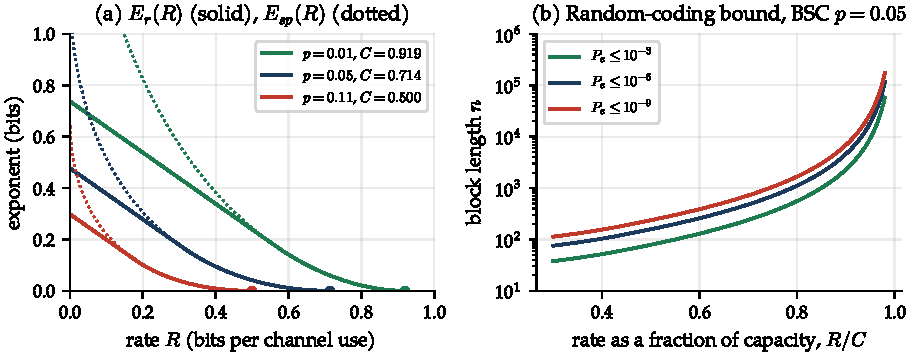
\includegraphics[width=0.92\linewidth]{figs/ch13_error_exponent}\caption{(a) Gallager's random-coding exponent $E_r(R)$ (solid) and the
sphere-packing exponent $E_{sp}(R)$ (dotted) for binary symmetric channels; they coincide above the
critical rate. (b) The block length at which the random-coding bound $2^{-nE_r(R)}$ guarantees a
given block error probability on a BSC with $p=0.05$ ($C=0.714$). Operating close to capacity
demands long blocks.}\label{fig:ch13_error_exponent}\end{figure}

The exponent explains the engineering trade-off between rate, reliability and delay.
Figure~\ref{fig:ch13_error_exponent}(b) turns it into block lengths. At half of capacity about
160 channel uses suffice for a block error rate of $10^{-6}$; at 90\% of capacity the bound asks
for about 4600; and near capacity $E_r(R)\approx(C-R)^2/(2V\ln2)$ for a constant $V$
(the dispersion of the next subsection), so the required length grows like $1/(C-R)^2$. Every
extra step towards capacity costs disproportionately more block length, and therefore more latency
and memory. That is why systems with tight latency budgets---voice, control loops, the
ultra-reliable low-latency communications (URLLC) of 5G---must sit further from capacity than
bulk-data links, and why finite-blocklength theory has become important.

\mdcfig{ch13_info_density}{The fuel gauge of a short code. On a BSC with $p=0.11$, the information a
block actually delivers (the average information density over the block) is random. Over 100 uses it
spreads by about $\pm0.1$ bit around $C=0.5$; over 1000 uses by only $\pm0.03$. A code that must work
in all but a fraction $\epsilon$ of blocks must aim below the left tail, and the tail is wider for
short blocks.}

\subsection{The finite-blocklength regime}
\label{sec:ch13:fbl}

Exponents describe the error probability at a fixed rate. The modern question is the reverse: at
a given block length $n$ and target error probability $\epsilon$, what is the highest rate? In
2010 Yury Polyanskiy, H.~Vincent Poor and Sergio Verd\'u gave tight bounds and a remarkably accurate
approximation, refining a 1962 result of Volker Strassen:
\begin{equation}
R^*(n,\epsilon)\approx C-\sqrt{\frac Vn}\,\Q^{-1}(\epsilon)+\frac{\log_2n}{2n}.
\label{eq:ch13:normal}
\end{equation}
The new quantity is the \term{channel dispersion} $V$, the variance of the information density
$\log_2[W(Y\mid X)/p(Y)]$ under the capacity-achieving input. The formula has the shape of a
Gaussian confidence interval, and that is exactly what it is.

\begin{analogy}[A fuel tank for a short trip]
Plan a long road trip and you can budget fuel by the car's average consumption: over a thousand
kilometres the hills and headwinds average out. Plan a ten-kilometre trip up a mountain pass and
you had better carry a margin, because one steep stretch can dominate. A short codeword is the
short trip: in $n$ channel uses the channel's ``information content'' fluctuates with standard
deviation $\sqrt{nV}$, and a code that must succeed with probability $1-\epsilon$ must back off by
$\Q^{-1}(\epsilon)$ standard deviations. The shorter the trip and the stricter the deadline, the
bigger the margin.
\end{analogy}

Figure~\ref{fig:ch13_info_density} simulates the fuel gauge: twenty thousand blocks of a BSC, and
for each the information it actually delivered. The spread shrinks like $1/\sqrt n$, exactly the
$\sqrt{V/n}$ of~\eqref{eq:ch13:normal}.

For the real Gaussian channel at SNR $P$, $C=\frac12\log_2(1+P)$ and
$V=\frac{P(P+2)}{2(P+1)^2}\log_2^2e$; for the BSC, $V=p(1-p)\log_2^2\frac{1-p}{p}$.

\mdcfig{ch13_finite_blocklength}{The finite-blocklength penalty on the real Gaussian channel,
from the normal approximation~\eqref{eq:ch13:normal}. (a) The maximum rate at SNR $=0$\,dB
($C=0.5$) as a function of block length for several block error probabilities $\epsilon$. (b) The
extra SNR, above Shannon's value, needed to carry rate 0.5 or 1 bit per real channel use in a block
of $n$ uses. Short, very reliable packets pay several decibels.}

Figure~\ref{fig:ch13_finite_blocklength} shows what this means. At SNR $=0$\,dB, where capacity is
0.5 bits per real channel use, a block of 100 uses with $\epsilon=10^{-5}$ can carry only about
0.16 bits per use; 1000 uses, about 0.39; 10\,000 uses, about 0.46. Put differently, to carry rate
0.5 with $\epsilon=10^{-5}$ costs 3.8\,dB more than Shannon's figure at $n=100$, 1.3\,dB at
$n=1000$ and 0.4\,dB at $n=10\,000$. For packets of a few hundred bits the finite-length penalty is
larger than the entire gap between a good practical code and the asymptotic limit.

\begin{worked}[The URLLC packet]
The 5G requirement for ultra-reliable low-latency communications, set out in 3GPP TR 38.913, is a
32-byte packet delivered with success probability $1-10^{-5}$ within 1\,ms. Suppose the 256
information bits are sent in $n=512$ real channel uses (256 QPSK symbols, rate $\frac12$ per real
dimension). Shannon's asymptotic formula says rate $\frac12$ needs $E_b/N_0=0$\,dB. The normal
approximation says that with $n=512$ and $\epsilon=10^{-5}$ it needs about 1.8\,dB. Spreading the
same 256 bits over 1024 or 2048 real uses (a lower-rate code in more bandwidth) brings the
requirement down to about 1.0 and 0.6\,dB, but those must be compared with asymptotic limits of
$-0.8$ and $-1.2$\,dB: the penalty stays near 1.8\,dB, because it is set mainly by the number of
information bits and the reliability target (Figure~\ref{fig:ch13_urllc}). Real URLLC designs therefore combine several tools:
they add diversity (frequency, antennas, repetitions) so that fading does not dominate
(Section~\ref{sec:ch13:fading}), use short LDPC or polar codes that come within a few tenths of a
decibel of~\eqref{eq:ch13:normal}, and budget the rest as link margin.
\end{worked}

\mdcfig{ch13_urllc}{The URLLC packet of the worked example in numbers: the $E_b/N_0$ needed to
deliver 256 information bits with block error probability $10^{-5}$, for three code lengths, against
Shannon's infinite-length figure at the same rate. Lowering the rate helps both, but the
short-packet penalty stays near 1.8\,dB.}

\begin{inpractice}[Short codes in 5G and IoT]
The finite-blocklength view changed how codes are chosen. For long transport blocks, 5G NR uses
LDPC codes whose performance at a few thousand bits is within about a decibel of the
normal approximation. For control information---a few dozen bits of scheduling grants and
acknowledgements---it uses polar codes with CRC-aided successive-cancellation list decoding, which
at these lengths come closer to the finite-length bound than turbo or LDPC codes of the same size
(3GPP TS 38.212). LoRa, NB-IoT and satellite IoT links, whose packets are often only tens of bytes,
operate at low SNR where each packet is a short code, and their designers use the normal
approximation to set realistic link budgets. The theory also has a sobering message for massive
machine-type communications: sending many tiny packets is intrinsically less efficient than
sending few large ones, whatever the code.
\end{inpractice}

\begin{tryit}[Feel the short-packet penalty]
In Lab 19's \emph{Finite blocklength} experiment, set the SNR to 0\,dB and drag the block-length
slider from 100\,000 down to 100 while watching the achievable rate. Then tighten the target error
probability from $10^{-1}$ to $10^{-9}$ at $n=200$. Which costs more: a ten-times shorter packet or
a ten-thousand-times stricter reliability target?
\end{tryit}

%======================================================================
\section{Continuous channels and the Gaussian channel}
\label{sec:ch13:awgn}
%======================================================================

Radio, cable and fibre channels have continuous-valued inputs and outputs. The theory extends to
them with one new ingredient, the entropy of a continuous random variable, and one famous
result, the capacity of the additive white Gaussian noise channel---the formula every engineer
knows, and the one that is quoted wrongly most often.

\subsection{Differential entropy}

For a continuous random variable with density $f(x)$, the \term{differential entropy} is
\begin{equation}
h(X)=-\int f(x)\log_2f(x)\,dx.
\label{eq:ch13:diffent}
\end{equation}
It behaves like entropy in most respects, with two important differences. First, it can be
negative: a uniform density on $[0,a]$ has $h=\log_2a$, which is negative for $a<1$. Second, it is
not invariant to scaling: $h(aX)=h(X)+\log_2|a|$. Both reflect the fact that a continuous variable
carries infinitely many bits if measured with infinite precision.

\mdcfig[0.5]{ch13_ruler}{The ruler made visible: the entropy of a unit-variance Gaussian quantised
with step $\Delta$ (dots) follows $h(X)-\log_2\Delta$ (line) once the step is fine. Each halving
of the step adds one bit.}

\begin{analogy}[The ruler]
How much information is in your height? It depends on the ruler. To the nearest metre, very
little; to the nearest millimetre, a few more bits; to the nearest atom, a great many. Differential
entropy is the part of the answer that does not depend on the ruler: quantise $X$ with a fine step
$\Delta$ and the entropy of the result is $H(X_\Delta)\approx h(X)-\log_2\Delta$. Halve the ruler's
step and you add exactly one bit, whatever $X$ is. Mutual information, as we shall see, subtracts
two such quantities measured with the same ruler, and the ruler cancels.
\end{analogy}

Figure~\ref{fig:ch13_ruler} checks the rule numerically: quantise a Gaussian ever more finely, and
its entropy climbs without limit, one bit per halving of the step, along a line offset by exactly
$h(X)=2.05$ bits.

Two useful examples:
\begin{align}
\text{uniform on an interval of width }a:&\quad h=\log_2a,\\
\text{Gaussian with variance }\sigma^2:&\quad h=\tfrac12\log_2\!\big(2\pi e\sigma^2\big).
\label{eq:ch13:hgauss}
\end{align}
For a Gaussian vector with covariance matrix $\mathbf{K}$ in $n$ dimensions,
$h=\frac12\log_2\big((2\pi e)^n\det\mathbf{K}\big)$, and for a circularly-symmetric complex Gaussian
of variance $\sigma^2$ (two real dimensions of $\sigma^2/2$ each) it is $\log_2(\pi e\sigma^2)$.

The good news is that \emph{mutual information} between continuous variables,
$I(X;Y)=h(Y)-h(Y\mid X)$, is perfectly well behaved: non-negative, invariant to any invertible
processing of $X$ or $Y$, and equal to the limit of the mutual information between finely quantised
versions. The ruler-dependent parts cancel.

\mdcfig[0.5]{ch13_gauss_maxent}{Three densities with the same unit variance. The Gaussian is
the most ``spread out'' in the information sense: its differential entropy beats the Laplace and
uniform densities.}

\subsection{The Gaussian maximises entropy}

Among all real random variables with variance $\sigma^2$, the Gaussian has the largest differential
entropy (Figure~\ref{fig:ch13_gauss_maxent}). The proof is Gibbs' inequality once more. Let $f$ be
any density with variance $\sigma^2$ and $\phi$ the Gaussian density with the same variance. Then
\begin{equation}
0\le D(f\|\phi)=\int f\log_2\frac f\phi=-h(f)-\int f\log_2\phi
=-h(f)+\tfrac12\log_2(2\pi e\sigma^2),
\label{eq:ch13:maxent}
\end{equation}
because $\log_2\phi(x)$ is a quadratic in $x$ whose average depends only on the variance, which $f$
and $\phi$ share. So $h(f)\le\frac12\log_2(2\pi e\sigma^2)$, with equality only for $f=\phi$.

This single fact has two faces in communications. On the noise side, Gaussian noise is the
\emph{worst} additive noise of a given power: it has the most entropy, so it destroys the most
information. A channel with non-Gaussian noise of the same power has at least the Gaussian
capacity, which is why the Gaussian channel is a safe, pessimistic design model. On the signal
side, a Gaussian \emph{input} carries the most information per unit power; any other input
distribution---including every practical constellation---leaves something on the table
(Section~\ref{sec:ch13:constrained}). Nature's most common noise is also its most destructive, and
its most destructive noise is also the best signal: the same bell curve plays hero and villain.

\begin{figure}[htbp]\centering
\begin{minipage}[t]{0.52\linewidth}\centering
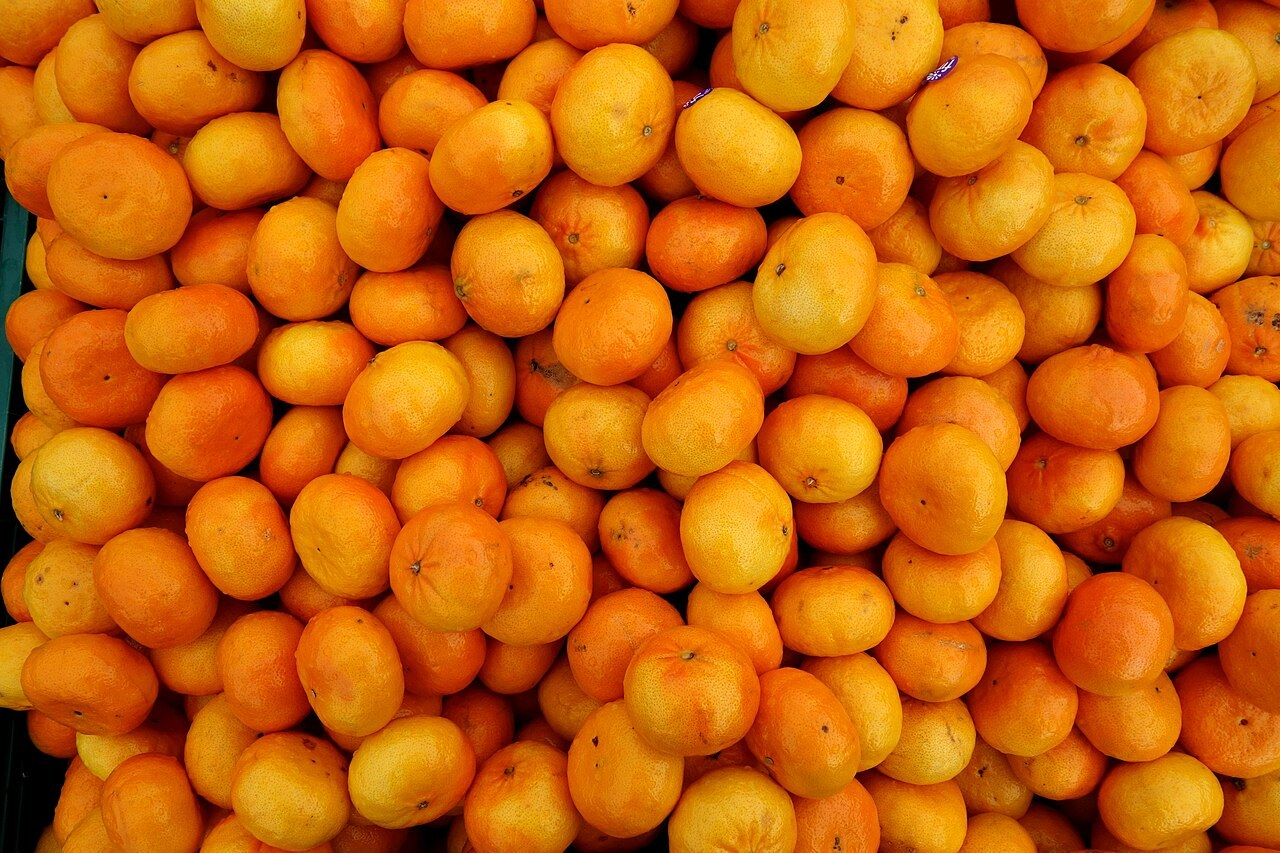
\includegraphics[width=\linewidth,height=4.9cm,keepaspectratio]{figs/photos/ch13_mandarins}
\caption{Mandarins heaped on a market stall. How many fit in the crate depends on the ratio of
the crate's volume to each fruit's.\mdccredit{ch13_mandarins}}
\label{fig:ch13_mandarins}\end{minipage}\hfill
\begin{minipage}[t]{0.44\linewidth}\centering
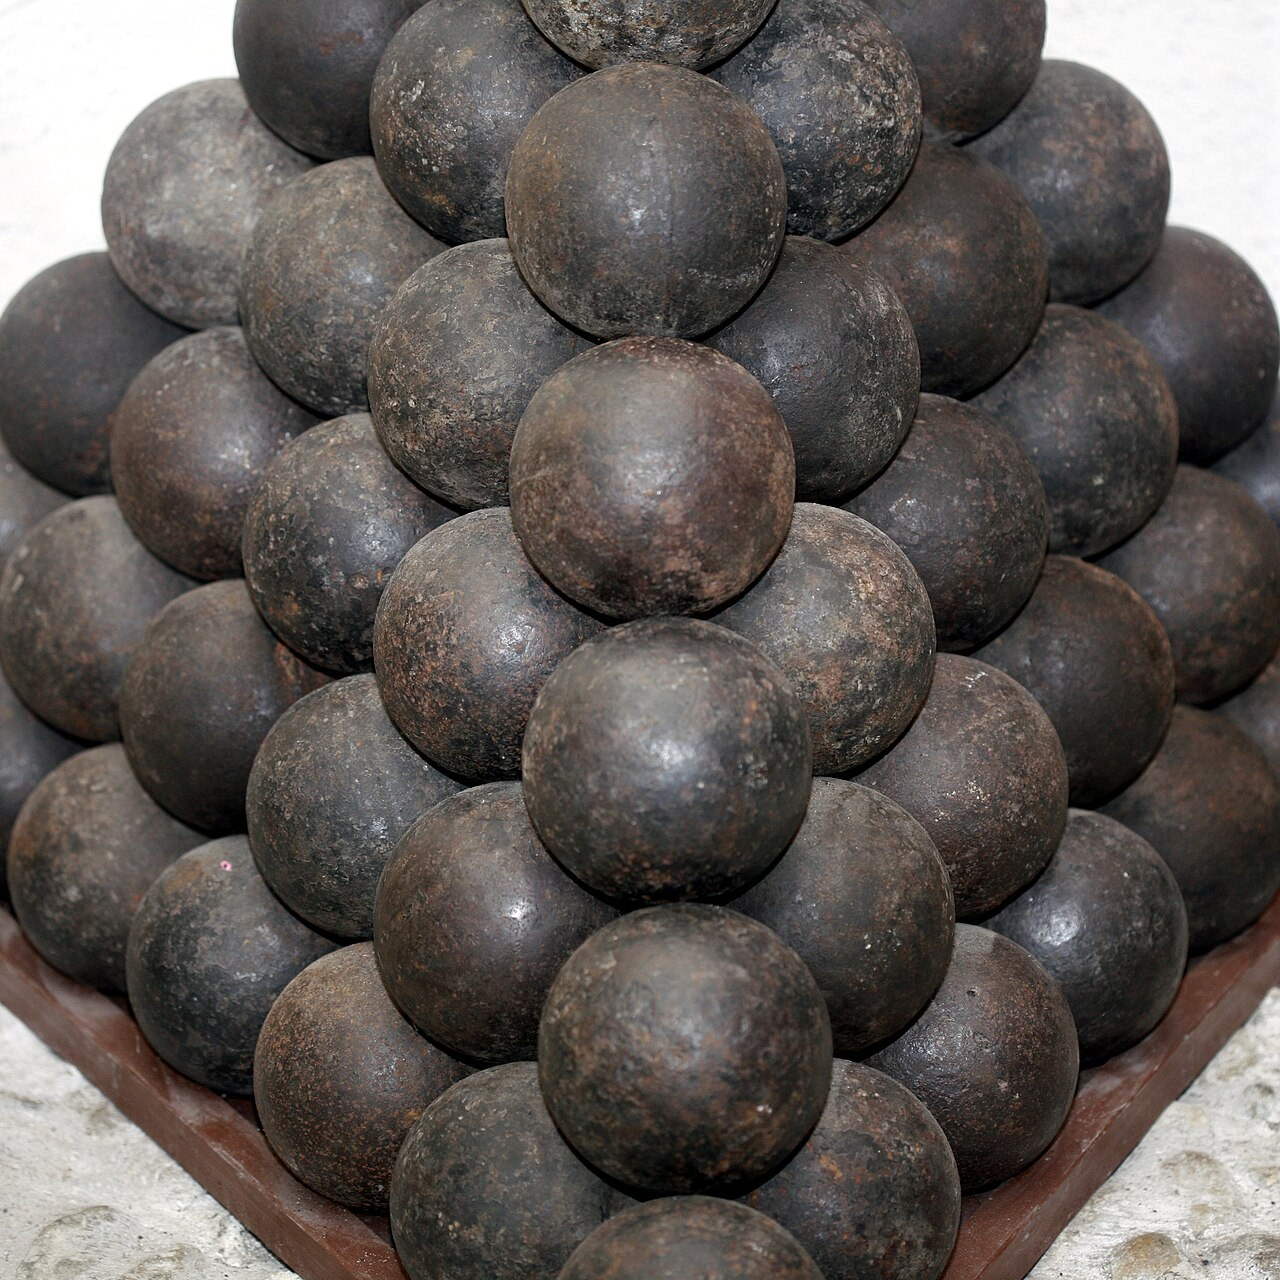
\includegraphics[width=\linewidth,height=4.9cm,keepaspectratio]{figs/photos/ch13_cannonballs}
\caption{Cannonballs stacked in a pyramid: the densest packing of equal spheres in three
dimensions, as Kepler conjectured in 1611; Thomas Hales announced a proof in 1998.\mdccredit{ch13_cannonballs}}
\label{fig:ch13_cannonballs}\end{minipage}
\end{figure}

\subsection{Capacity of the additive Gaussian channel}

Consider the discrete-time real channel $Y=X+Z$, with $Z\sim\mathcal{N}(0,N)$ independent of the
input and an average power constraint $\E[X^2]\le P$. The derivation is three short steps. Given
$X$, the output is $X$ plus noise, so $h(Y\mid X)=h(Z)=\frac12\log_2(2\pi eN)$. The output has
variance at most $P+N$, so by the maximum-entropy property $h(Y)\le\frac12\log_2(2\pi e(P+N))$.
Therefore
\begin{equation}
I(X;Y)=h(Y)-h(Z)\le\tfrac12\log_2\!\Big(1+\frac PN\Big),
\label{eq:ch13:awgnbound}
\end{equation}
and a Gaussian input $X\sim\mathcal{N}(0,P)$ makes $Y$ Gaussian and achieves equality. The capacity
of the real AWGN channel is
\begin{equation}
C=\frac12\log_2\!\Big(1+\frac PN\Big)\quad\text{bits per real channel use}.
\label{eq:ch13:awgn}
\end{equation}
For a complex baseband channel with circularly-symmetric noise, which is two real channels in
parallel sharing the power, $C=\log_2(1+P/N)$ bits per complex use.

\subsection{The geometric picture: oranges in a thousand dimensions}

Shannon's 1949 paper ``Communication in the presence of noise'' derived the same formula from a
picture, and the picture is worth more than the algebra. It starts in the greengrocer's.

\begin{analogy}[Oranges in a crate]
How many oranges fit in a crate? Roughly the volume of the crate divided by the volume of one
orange (a bit less, because round things leave gaps). Shannon's capacity formula is exactly that
calculation, done for codewords. Each codeword is the centre of an ``orange'' of noise: the
region of space where the received signal is likely to land. The crate is the region of all
received signals. The number of distinguishable messages is the number of oranges that fit
without squashing each other. The analogy's surprise, which only mathematics can show, is that
in very many dimensions the oranges become all peel (Figure~\ref{fig:ch13_shell_volume}) and the
gaps between them become negligible.
\end{analogy}

Think of a block of $n$ channel uses as a single point in $n$-dimensional space. The noise vector
$\mathbf{z}$ has $n$ independent components of variance $N$, so $\|\mathbf{z}\|^2$ is a sum of $n$
independent terms whose average is $nN$. By the law of large numbers, $\|\mathbf{z}\|\approx\sqrt{nN}$
with relative fluctuations that shrink like $1/\sqrt n$: in high dimensions the noise does not fill
a ball, it lives on a thin shell. This \term{sphere hardening}
(Figure~\ref{fig:ch13_sphere_hardening}(b)) is the geometric form of the AEP. Each transmitted
codeword $\mathbf{x}$, with $\|\mathbf{x}\|^2\le nP$, is received somewhere on a thin shell of radius
$\sqrt{nN}$ around it; and all received vectors lie within a ball of radius $\sqrt{n(P+N)}$.

\mdcfig[0.5]{ch13_shell_volume}{High-dimensional oranges are all peel: the fraction of an
$n$-dimensional ball's volume lying in a thin outer shell, $1-(1-\epsilon)^n$, tends to one as $n$
grows.}

Why a shell? Because volume in high dimensions lives at the edge. The volume of an
$n$-dimensional ball grows as $r^n$, so the fraction of it within the outer 5\% of the radius is
$1-0.95^n$: 14\% in three dimensions, 99.4\% in a hundred (Figure~\ref{fig:ch13_shell_volume}). A
hundred-dimensional orange is 99.4\% peel. Noise vectors, like everything else, fall where the
volume is, which is why their length is so predictable---and why a decoder that looks for the
codeword at distance about $\sqrt{nN}$ from what it received almost never finds the wrong one.
This is the deepest reason that long codes work and short codes struggle: only in high dimensions
does noise become predictable enough to be outwitted.

\mdcfig{ch13_sphere_hardening}{(a) Shannon's sphere-packing picture, drawn in two dimensions for
want of more. Codewords (dots) lie inside the ball of received signals, of radius
$\sqrt{n(P+N)}$; around each is a noise sphere of radius $\sqrt{nN}$, and reliable decoding requires
the noise spheres not to overlap. (b) Sphere hardening: the length of an $n$-dimensional Gaussian
noise vector, normalised by $\sqrt{nN}$, concentrates at 1 as $n$ grows. In high dimensions the
noise sphere is a thin shell with a sharp edge.}

Reliable decoding requires that the noise spheres around different codewords do not overlap. The
volume of an $n$-dimensional ball of radius $r$ is proportional to $r^n$, so the number of
non-overlapping noise spheres that fit into the ball of received signals is at most
\begin{equation}
M\le\frac{\big(\sqrt{n(P+N)}\big)^n}{\big(\sqrt{nN}\big)^n}=\Big(1+\frac PN\Big)^{n/2},
\qquad
\frac{\log_2M}{n}\le\frac12\log_2\!\Big(1+\frac PN\Big).
\label{eq:ch13:spheres}
\end{equation}
This is the converse: crate volume over orange volume. The achievability half says that codewords
chosen at random on the sphere of radius $\sqrt{nP}$ pack almost this well---in high dimensions
random points are nearly as good as the best arrangement---so the bound is reached. The ``1+'' in
the formula comes from the signal and noise volumes adding; the ``$\frac12$'' from the square root
relating radius to power.

\subsection{The band-limited channel: $C=B\log_2(1+\mathrm{SNR})$}

A continuous-time channel of bandwidth $B$\,Hz offers, by the sampling theorem, $2B$ independent
real dimensions per second (strictly, a signal of duration $T$ and bandwidth $B$ has approximately
$2BT$ degrees of freedom, a statement made precise by Landau, Pollak and Slepian in the 1960s).
White noise of two-sided density $N_0/2$ puts variance $N_0/2$ in each dimension, and a signal of
power $P$ spreads $P/2B$ into each. Multiplying~\eqref{eq:ch13:awgn} by $2B$ dimensions per second,
\begin{equation}
C=B\log_2\!\Big(1+\frac{P}{N_0B}\Big)=B\log_2(1+\mathrm{SNR})\quad\text{bits per second},
\label{eq:ch13:shannonhartley}
\end{equation}
the \term{Shannon--Hartley theorem}, the most famous formula in communications
(Chapter~\ref{ch:history} introduced it as Equation~\eqref{eq:ch01:shannon}). The SNR is measured
in the signal bandwidth. In complex-baseband language, a bandwidth $B$ supports $B$ complex symbols
per second, each carrying at most $\log_2(1+\mathrm{SNR})$ bits. In words: \emph{bandwidth buys
you symbols; SNR buys you bits per symbol, but only logarithmically}.

\mdcfig{ch13_bw_vs_power}{Bandwidth or power? Start from a 10\,MHz channel at 20\,dB SNR (67\,Mb/s).
Doubling the transmit power adds only 10\,Mb/s; doubling the bandwidth with the same total power
adds 46\,Mb/s, more than multiplying the power by ten. At high SNR, bandwidth is the stronger lever.}

Figure~\ref{fig:ch13_bw_vs_power} puts numbers on the slogan. It is why spectrum auctions raise
billions and why every cellular generation has reached for wider channels: at high SNR, a hertz is
worth far more than a watt.

\begin{history}[A formula with several fathers]
The formula~\eqref{eq:ch13:shannonhartley} is often called Shannon--Hartley, although Hartley never
wrote it; his 1928 rule counted distinguishable levels, not probabilities, and had no notion of a
limit achieved by coding. In 1948--49 several people reached similar expressions: William Tuller at
MIT in a 1949 paper, Jacques Laplume in a 1948 note to the French Academy of Sciences, and others
using heuristic ``levels-within-noise'' arguments of the form $\log_2(1+A/\Delta)$. What
distinguished Shannon's result was the operational meaning. The others gave a plausible count of
distinguishable signals; Shannon proved that rates below $C$ are achievable with vanishing error
probability and rates above it are not. The formula's widespread fame came partly through Warren
Weaver, who wrote an accessible introduction for the 1949 book edition, retitled \emph{The}
Mathematical Theory of Communication---a change of article that signalled how quickly the theory
had been accepted as definitive. Shannon himself grew wary of the enthusiasm and in a 1956
editorial, ``The bandwagon'', warned against applying information theory indiscriminately to
psychology, economics and biology.
\end{history}

\subsection{Two regimes}
\mdcfig{ch13_awgn_capacity}{(a) Capacity per hertz of the AWGN channel against SNR, with its
high-SNR (logarithmic) and low-SNR (linear) approximations. Two operating points used in this
chapter's worked examples are marked. (b) Capacity at fixed received power $P$ as the bandwidth
grows: it saturates at $C_\infty=(P/N_0)\log_2e$. Half of the ultimate capacity is already reached
at $B\approx0.1P/N_0$, and 90\% by $B\approx4P/N_0$.}


The logarithm makes~\eqref{eq:ch13:shannonhartley} behave very differently at low and high SNR
(Figure~\ref{fig:ch13_awgn_capacity}(a)).
\begin{description}[style=nextline,leftmargin=1.2em,font=\sffamily\bfseries\small\color{navy}]
\item[High SNR: bandwidth-limited.] For $\mathrm{SNR}\gg1$, $C\approx B\log_2\mathrm{SNR}$. Capacity
grows only logarithmically with power: every doubling of power (3\,dB) buys one more bit per second
per hertz, but doubling the bandwidth nearly doubles the capacity. Here bandwidth is the precious
resource. Cellular, Wi-Fi, cable, microwave backhaul and coherent optics live in this regime.
\item[Low SNR: power-limited.] For $\mathrm{SNR}\ll1$, $\ln(1+x)\approx x$ gives
$C\approx B\cdot\mathrm{SNR}\cdot\log_2e=(P/N_0)\log_2e$. Capacity is \emph{linear} in power and
nearly independent of bandwidth. Here every decibel of received power is precious and bandwidth is
cheap. Deep-space probes, GNSS and low-power IoT live in this regime.
\end{description}

Figure~\ref{fig:ch13_awgn_capacity}(b) shows the same trade-off at fixed power. As bandwidth grows,
the SNR per hertz falls, and capacity climbs towards the asymptote
\begin{equation}
C_\infty=\lim_{B\to\infty}B\log_2\!\Big(1+\frac P{N_0B}\Big)=\frac P{N_0}\log_2e\approx1.44\,\frac P{N_0}.
\label{eq:ch13:cinf}
\end{equation}
Infinite bandwidth does not give infinite capacity. It gives $1.44$ bits per second for every
unit of $P/N_0$, and no more: spread a fixed power thinly enough and each hertz carries almost
nothing.

\mdcfig{ch13_ebn0_limit}{The minimum energy per bit~\eqref{eq:ch13:ebn0} as a function of spectral
efficiency. Below $\eta\approx0.1$ the curve is flat at the Shannon limit: spending more bandwidth
saves almost no energy. Above $\eta=1$ each extra bit per hertz costs about 3\,dB.}

\subsection{The Shannon limit: $-1.59$\,dB}

Writing the received power as the energy per bit times the bit rate, $P=E_bR$, and setting $R=C$
in~\eqref{eq:ch13:shannonhartley} with spectral efficiency $\eta=C/B$, gives
\begin{equation}
\eta=\log_2\!\Big(1+\eta\frac{E_b}{N_0}\Big)
\qquad\Longleftrightarrow\qquad
\frac{E_b}{N_0}=\frac{2^\eta-1}{\eta}.
\label{eq:ch13:ebn0}
\end{equation}
This is the minimum energy per bit at spectral efficiency $\eta$, already met in
Chapter~\ref{ch:modulation}. It is 0\,dB at $\eta=1$, 1.76\,dB at $\eta=2$, 10.2\,dB at
$\eta=6$, and it rises by about 3\,dB per extra bit per hertz at high $\eta$. As $\eta\to0$ it
decreases to
\begin{equation}
\left.\frac{E_b}{N_0}\right|_{\min}=\ln2=0.693=-1.59\,\text{dB},
\label{eq:ch13:limit}
\end{equation}
the \term{Shannon limit}. No system, however much bandwidth it uses and however complex its code,
can communicate reliably through white Gaussian noise with less than $0.693\,N_0$ joules per bit.
At room temperature ($N_0=kT_0=4\times10^{-21}$\,W/Hz) that is $2.8\times10^{-21}$\,J per bit,
about $0.017$\,eV---a number that also appears in the thermodynamics of computing as Landauer's
bound, $kT\ln2$ per bit erased.

Figure~\ref{fig:ch13_ebn0_limit} shows the whole curve. Its two halves are the two regimes of the
previous subsection seen from the energy side: a flat floor on the left, where bandwidth is
plentiful and energy is everything, and a steep wall on the right, where squeezing more bits into
each hertz becomes exponentially expensive.

\begin{analogy}[The four-minute mile that can never be broken]
For decades runners treated the four-minute mile as a wall; on 6 May 1954 Roger Bannister ran
3:59.4 in Oxford, and within a few years many others had followed. Coding theorists had their own
four-minute mile: for forty years after 1948, getting within a decibel or two of Shannon's limit
seemed beyond reach, until turbo codes did it in 1993 and the record tumbled. But the analogy
breaks in an instructive way. Bannister's barrier was psychological and physiological, and
records keep falling. Shannon's barrier is mathematical: $-1.59$\,dB will \emph{never} be beaten,
any more than a perpetual-motion machine will be built. Coding gains are always measured
\emph{towards} it, never through it.
\end{analogy}

\begin{keyidea}[The two currencies and their exchange rate]
Every link spends two currencies: bandwidth and energy per bit. Shannon's
curve~\eqref{eq:ch13:ebn0} is the exchange rate between them. In the power-limited regime, halving
the spectral efficiency saves almost nothing once $\eta$ is well below 1 (the curve is flat near
$-1.59$\,dB). In the bandwidth-limited regime, each extra bit per hertz costs about 3\,dB. A
designer who knows which regime the link is in knows immediately whether to spend effort on
bandwidth, on power or on the code.
\end{keyidea}

\mdcfig{ch13_modem_history}{Forty years of voice-band modems against Shannon's ceiling for an
analog telephone channel. Each standard squeezed more out of the same 3.1\,kHz until V.34 reached
93\% of capacity; V.90's 56\,kb/s (green) only looks like a violation, because it uses a different
channel model (see the worked example).}

Figure~\ref{fig:ch13_modem_history} tells the story of the most-studied channel in history, and
the worked example explains its ending.

\begin{worked}[The telephone line and the 56k modem]
A voice-band telephone channel passes roughly 300\,Hz to 3400\,Hz, a bandwidth of about
3.1\,kHz, and a good end-to-end connection in the 1990s offered an SNR of about 35\,dB (limited
mostly by the $\mu$-law quantisation in the digital network, Chapter~\ref{ch:pcm}). Shannon's
formula gives
\[
C=3100\log_2\big(1+10^{3.5}\big)=3100\times11.63=36.0\ \text{kb/s}.
\]
The V.34 modem (1994, extended to 33.6\,kb/s in 1996) used adaptive symbol rates up to 3429\,baud,
trellis-coded modulation, shell-mapping constellation shaping, precoding and line probing to
reach 33.6\,kb/s---about 93\% of this figure on a good line. It was the end of the road for modems
that treated the telephone network as an analog channel.

Then V.90 (1998) delivered 56\,kb/s downstream over the same lines. Shannon was not broken; the
\emph{model} changed. The dominant ``noise'' in the voice path was the quantisation error of the
network's 8-bit PCM codec. When the server connects to the network digitally, the downstream signal
is \emph{already} a stream of PCM codes, and a V.90 modem chooses its constellation points to be
exactly the codec's output levels: 8000 symbols per second, up to 7 bits each. Quantisation noise
aligned with the constellation is not noise at all. The remaining limits---a subset of levels too
close together near zero, and regulatory limits on transmitted power---held practical downstream
rates to about 53\,kb/s. The upstream, which still passed through an analog-to-PCM conversion,
stayed at V.34 rates. Capacity belongs to a channel model; change the model and you change the
capacity.
\end{worked}

\mdcphoto[0.45]{ch13_voyager}{Voyager in flight (NASA artist's impression). Its 3.7\,m dish and roughly 20-watt
transmitter make every deep-space link a power-limited channel, where each decibel of coding
gain is worth a quarter more data.}

Deep space is the purest example of the power-limited regime, and the place where Shannon's limit
stopped being an abstraction and became a budget line. A probe beyond Saturn has a fixed,
modest transmitter, a dish only a few metres across and a distance measured in light-hours; the
ground station can make its antenna bigger and its receiver colder, but at some point the only
remaining lever is the code. Bandwidth, by contrast, is plentiful: nobody else is transmitting
from the outer solar system. Every generation of deep-space mission has therefore been an early
customer for the best codes of its day, from the Mariner probes' Reed--Muller code to the
concatenated codes of Voyager, the turbo codes standardised by CCSDS and today's LDPC codes. The
worked example puts numbers on the payoff.

\begin{worked}[A deep-space link at the edge]
A spacecraft far beyond Saturn delivers a received carrier-to-noise density of
$P/N_0=50$\,dB-Hz to a large ground antenna (a Voyager-like situation; the value is illustrative).
Whatever the bandwidth, the ultimate capacity~\eqref{eq:ch13:cinf} is
$C_\infty=10^5\times1.443=144$\,kb/s. What can real systems get?
\begin{itemize}
\item Uncoded BPSK needs $E_b/N_0\approx9.6$\,dB for $P_b=10^{-5}$, so $R=10^5/10^{0.96}=11$\,kb/s,
8\% of the limit.
\item A concatenated Reed--Solomon plus $K=7$ convolutional code of the Voyager era needs about
2.5\,dB: $R=10^5/10^{0.25}=56$\,kb/s.
\item A modern turbo or LDPC code at low rate needing about 0.5\,dB would reach roughly 89\,kb/s.
\end{itemize}
Each decibel of coding gain is worth 26\% more data from the edge of the solar system, which is
why deep-space missions were the first customers of every new generation of codes. The remaining
gap to 144\,kb/s is the 2\,dB between 0.5\,dB and the $-1.59$\,dB limit, reachable only with
vanishing rate and unbounded bandwidth.
\end{worked}

\begin{figure}[H]\centering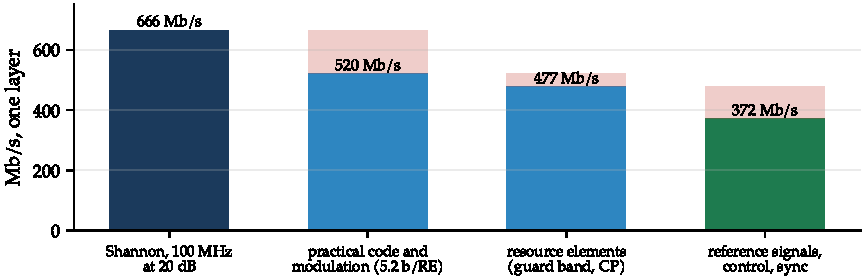
\includegraphics[width=0.85\linewidth]{figs/ch13_nr_budget}\caption{Where Shannon's 666\,Mb/s goes on a 100\,MHz 5G carrier at 20\,dB (one
layer; the numbers of the worked example). The red ghosts are the losses: a practical code and
constellation backed off from capacity, guard bands and cyclic prefix, and the reference, control
and synchronisation signals that make the link work at all.}\label{fig:ch13_nr_budget}\end{figure}

\begin{worked}[A 100\,MHz 5G carrier at 20\,dB]
A 5G NR carrier of 100\,MHz serves a user at an SNR of 20\,dB. With one spatial layer,
\[
C=100\times10^6\log_2(1+100)=100\times6.66=666\ \text{Mb/s}.
\]
What does the real system deliver? At 30\,kHz subcarrier spacing, 273 resource blocks occupy
98.3\,MHz. At 20\,dB the link adaptation chooses roughly 256-QAM at a code rate
near 0.65, or 64-QAM near the top of its range: about 5.2 information bits per resource element,
which corresponds to operating some 4\,dB below Shannon's 6.66 once practical code lengths, the
10\% block-error target of the first transmission and channel-estimation losses are counted. With
14 OFDM symbols per 0.5\,ms slot (the cyclic prefix costs about 7\%), the carrier offers
$3276\times28\,000\approx91.7$ million resource elements per second, and reference signals,
control channels and synchronisation blocks consume very roughly 20--25\% of them. The result is
on the order of $91.7\times5.2\times0.78\approx370$\,Mb/s per layer, a little over half of
Shannon's figure (Figure~\ref{fig:ch13_nr_budget}). Four MIMO layers (Section~\ref{sec:ch13:mimo}) multiply the ceiling
and the achieved rate by up to about four. The ``missing'' half is not waste: overheads buy
synchronisation, channel estimation and multi-user control, and the backoff buys robustness to a
channel that changes every millisecond.
\end{worked}

%======================================================================
\section{The spectral-efficiency plane and real systems}
\label{sec:ch13:plane}
%======================================================================

Equation~\eqref{eq:ch13:ebn0} divides the plane of $E_b/N_0$ and spectral efficiency into the
achievable and the impossible, like a map with a coastline: everything to the left of the red
curve is sea. Chapter~\ref{ch:modulation} placed the \emph{uncoded} modulations on that map
(Figure~\ref{fig:ch09_efficiency_plane}); Figure~\ref{fig:ch13_efficiency_plane} adds a real coded
system. The markers are the 28 modulation and coding combinations of the DVB-S2 satellite
broadcasting standard, at the $E_s/N_0$ values that ETSI EN 302 307 lists for quasi-error-free
operation (packet error rate about $10^{-7}$) with 64\,800-bit LDPC codes.

\mdcfig{ch13_efficiency_plane}{The spectral-efficiency plane with a real system on it. The red
curve is Shannon's bound~\eqref{eq:ch13:ebn0}; dashed curves are the limits for QPSK, 16-QAM and
64-QAM inputs (Section~\ref{sec:ch13:constrained}); crosses mark uncoded Gray-labelled QAM at
$P_b=10^{-5}$. Open markers are the DVB-S2 modulation and coding modes, from the ideal $E_s/N_0$
values listed in ETSI EN 302 307-1 (AWGN, normal 64\,800-bit frames, quasi-error-free) converted
to $E_b/N_0$. The whole family sits about 1 to 3\,dB from the bound, where uncoded modulation sits
8 to 10\,dB away.}

Three things stand out. First, the gap has collapsed: where uncoded QAM sits 8 to 10\,dB from
the bound, DVB-S2's QPSK rate-$\frac12$ mode needs $E_s/N_0=1.0$\,dB for 0.99\,bits per symbol,
only 1.1\,dB more than Shannon's minimum for that efficiency, and about 0.9\,dB more than the limit
for QPSK inputs. Second, the gap grows at the top of each constellation's range: rate-9/10 QPSK is
2.5\,dB from Shannon, because it runs close to QPSK's 2-bit ceiling where the constellation, not
the code, is the bottleneck. This is why the standard switches to 8-PSK, then 16- and 32-APSK, as
the SNR rises, and why a well-designed adaptive system operates each constellation at roughly 60 to
85\% of its maximum rate. Third, the power-limited modes pile up near $E_b/N_0\approx0.5$--1\,dB:
lowering the rate further buys little, as the flatness of Shannon's curve predicts. DVB-S2X, the
2014 extension, added lower rates (for mobile and very small terminals) and finer steps, and
reaches down to about $-10$\,dB $E_s/N_0$ using spreading-like very-low-rate modes.

\begin{inpractice}[Reading a standard's performance table]
Standards such as DVB-S2 (ETSI EN 302 307), DVB-S2X, ATSC~3.0 and CCSDS publish required
$E_s/N_0$ values for each mode. Treat them as the \emph{ideal} performance in AWGN with perfect
synchronisation. Real receivers add implementation losses of a few tenths of a decibel to a
decibel (phase noise, finite-precision demapping, imperfect channel estimation), and satellite
links add nonlinear distortion from the transponder's power amplifier
(Chapter~\ref{ch:satellite}). The capacity curve is the ruler against which all of these are
measured: when a link underperforms, the first question is how many decibels are lost to the code,
how many to the constellation, and how many to the implementation.
\end{inpractice}

%======================================================================
\section{Capacity with real constellations}
\label{sec:ch13:constrained}
%======================================================================

Shannon's formula assumes a Gaussian input: a transmitter that can send any real number, with
bell-curve statistics. Real transmitters send points from a finite menu: BPSK, QPSK, 16-QAM,
256-QAM, APSK. What is the capacity when the input is constrained to such a set, and how much do
we lose by choosing from a menu?

\mdcfig{ch13_constrained}{(a) Coded-modulation capacity of BPSK, QPSK, 8-PSK and square QAM
against the Gaussian-input capacity $\log_2(1+E_s/N_0)$. Each curve follows Shannon's closely
until it saturates at $\log_2M$. (b) The extra SNR a uniformly used square QAM constellation needs,
compared with a Gaussian input, to support a given rate. At moderate rates the loss is a few tenths
of a decibel; as the rate grows (using larger constellations) it approaches the shaping loss of
1.53\,dB.}

\subsection{Coded-modulation capacity}

Let the input be drawn uniformly from a constellation $\mathcal{X}$ of $M$ points with unit average
energy, and let $Y=X+Z$ with complex Gaussian noise of variance $N_0$, so that the SNR is
$E_s/N_0=1/N_0$. The mutual information, sometimes called the \term{coded-modulation capacity} or
constellation-constrained capacity, is
\begin{equation}
C_{\mathcal{X}}=\log_2M-\frac1M\sum_{x\in\mathcal{X}}\E_Z\!\left[\log_2\sum_{x'\in\mathcal{X}}
\exp\!\left(-\frac{|x+Z-x'|^2-|Z|^2}{N_0}\right)\right].
\label{eq:ch13:cm}
\end{equation}
Read it as ``the $\log_2M$ bits you put in, minus the average confusion the noise leaves about
which point was sent''. The confusion term counts, for each transmitted point, how plausible the
other points look from where the received sample landed.

\begin{deeper}[Where~\eqref{eq:ch13:cm} comes from, and how to compute it]
$I(X;Y)=H(X)-H(X\mid Y)$ with $H(X)=\log_2M$. The second term is the average of $\log_2$ of the
ratio of the total likelihood $\sum_{x'}p(y\mid x')$ to the likelihood $p(y\mid x)$ of the
transmitted point; after cancelling the Gaussian normalisation, that ratio is the sum inside the
expectation. The expectation over $Z$ has no closed form, but it is easily computed: by Monte
Carlo, or, for square QAM, exactly by Gauss--Hermite quadrature on each real dimension, because
square QAM is two independent PAM constellations in quadrature. The chapter's figure script does
both, using the constellations of \texttt{commlib.modulation.get\_constellation}.
\end{deeper}

Figure~\ref{fig:ch13_constrained}(a) shows the results. At low SNR every constellation is as good as
a Gaussian: when noise dominates, the fine structure of the input does not matter, and even BPSK
achieves $C\approx\mathrm{SNR}\log_2e$ per complex use (it uses only one of the two real
dimensions, so it follows the Gaussian curve only at very low SNR). As the SNR grows each curve
bends away from Shannon's and saturates at $\log_2M$, the entropy of the input: a 16-point menu can
never carry more than 4 bits, however clean the channel. The practical lesson is the ``60 to 85\%
rule'' seen in DVB-S2: operate a constellation where its curve is still close to the Gaussian one,
and move to a larger constellation before it saturates. From the curves: 16-QAM needs 5.1\,dB for
2 bits per symbol (0.35\,dB more than Shannon), 64-QAM needs 12.6\,dB for 4 bits (0.9\,dB more),
and 256-QAM needs 19.2\,dB for 6 bits (1.2\,dB more).

\subsection{The shaping gain: why 1.53\,dB?}

\mdcfig[0.42]{ch13_shaping}{Probabilistic shaping of 64-QAM: point areas proportional to their
probabilities (a Maxwell--Boltzmann distribution). Inner, low-energy points are used more often,
so the constellation ``looks'' more Gaussian; the entropy drops slightly below 6 bits, but the
energy drops more.}

Figure~\ref{fig:ch13_constrained}(b) shows that even a large square constellation used at a
comfortable fraction of its capacity stays a fixed distance from Shannon's curve. The reason is the
maximum-entropy property. A large, uniformly used square QAM constellation approximates a
\emph{uniform} density in each real dimension. For the same differential entropy---the same number
of bits per dimension---a uniform density on an interval of width $a$ has power $a^2/12$, whereas a
Gaussian with entropy $\log_2a$ has variance $a^2/(2\pi e)$. The ratio is
\begin{equation}
\frac{a^2/12}{a^2/(2\pi e)}=\frac{\pi e}6=1.423=1.53\,\text{dB},
\label{eq:ch13:shaping}
\end{equation}
the \term{shaping gain} that a uniform square grid gives up. In words: spending your power evenly
on all points wastes it on the expensive corner points. Recovering it requires either non-uniform
point spacing (geometric shaping) or non-uniform point probabilities (probabilistic shaping,
Figure~\ref{fig:ch13_shaping}), whose practice---from V.34's shell mapping to probabilistic
amplitude shaping in coherent optical transceivers---is described in
Section~\ref{sec:ch09:shaping}. In the geometric picture of Figure~\ref{fig:ch13_sphere_hardening},
a uniform square constellation fills a \emph{cube} in $n$ dimensions, while the ideal codebook
fills a \emph{sphere}; 1.53\,dB is the asymptotic ratio of their second moments. A cube is a
sphere with corners, and the corners are where the power goes to waste.

\mdcfig{ch13_bicm}{(a) Coded-modulation capacity (solid) and BICM capacity with Gray labelling
(dashed) for square QAM. (b) The SNR penalty of BICM relative to coded modulation at a given rate.
With Gray labels the loss is small where the constellation is used efficiently (upper part of each
curve) and larger at rates well below $\log_2M$; with natural binary labels (dotted, 16-QAM) it is
much larger. Computed by Gauss--Hermite quadrature and checked by Monte Carlo.}

\subsection{Bit-interleaved coded modulation}

Almost every modern wireless and broadcast standard---LTE, 5G NR, Wi-Fi, DVB-S2/T2, DOCSIS~3.1---uses
\term{bit-interleaved coded modulation} (BICM): one binary code, an interleaver and a Gray-labelled
mapper (Chapter~\ref{ch:modulation}). The receiver computes a log-likelihood ratio for each bit of
each symbol and hands them to a binary decoder that treats them as if they had come through $\log_2M$
independent binary channels. What rate can such a receiver support? Treating the bits
independently ignores the dependence between the bits of one symbol, and the
data-processing inequality says that can only lose information. The \term{BICM capacity} is the sum
of the mutual informations of the $m=\log_2M$ bit channels,
\begin{equation}
C_{\text{BICM}}=\sum_{i=1}^{m}I(B_i;Y)\;\le\;\sum_{i=1}^{m}I(B_i;Y\mid B_1,\ldots,B_{i-1})=C_{\mathcal{X}},
\label{eq:ch13:bicm}
\end{equation}
where the right-hand side, by the chain rule, is the full coded-modulation capacity. The chain-rule
form is also a recipe: \emph{multilevel coding} with multistage decoding, which decodes the bit
levels in order and uses earlier decisions to help later ones, achieves $C_{\mathcal{X}}$ exactly.

Figure~\ref{fig:ch13_bicm} measures the price. With Gray labelling, BICM loses less than 0.1\,dB
at the upper end of each constellation's useful range---the region where adaptive systems operate
it---but the loss grows at lower rates: at half the constellation's maximum rate it is 0.16\,dB
for 16-QAM, 0.4\,dB for 64-QAM and 0.7\,dB for 256-QAM. This is a second reason, beyond decoder
complexity, not to run a large constellation at a low code rate: switch to a smaller constellation
instead. With a poor labelling (natural binary) the loss can exceed 1.5\,dB, which is why the
labelling is specified in every standard. For the small residual loss, BICM buys the enormous
practical convenience of one binary code for every constellation, simple soft demapping, and
robustness to fading, which is why it displaced trellis-coded modulation in wireless systems
(Chapter~\ref{ch:modulation}). Iterative demapping (BICM-ID), in which the decoder's output is fed
back to the demapper, recovers part of the loss with non-Gray labels.

\mdcfig{ch13_gray_labels}{Why labelling matters for BICM, shown on 8-PAM. With Gray labels
(top) adjacent points differ in one bit (green), so the most likely symbol error costs one bit
error and each bit's LLR stays informative. With natural binary labels (bottom) some neighbours
differ in two or three bits (red), and bit-wise decoding pays for it.}

Figure~\ref{fig:ch13_gray_labels} shows the reason in one line of points: the bit-wise decoder
assumes each bit has its own clean channel, and Gray labelling comes closest to making that true.

\begin{inpractice}[How a 5G scheduler uses these curves]
A 5G NR base station chooses, every slot, a modulation and coding scheme (MCS) from tables in 3GPP
TS 38.214: QPSK to 256-QAM (and 1024-QAM in later releases) with code rates from about 0.03 to
0.93. The UE reports a channel quality indicator (CQI) derived from its measured SNR, and the
scheduler picks the MCS whose required SNR, roughly the BICM curve of
Figure~\ref{fig:ch13_bicm} plus a code gap of 1 to 2\,dB, fits the report with a margin tuned to hit
a 10\% first-transmission block error rate. Hybrid ARQ then cleans up the failures. The tables step
through constellations in exactly the pattern the capacity curves recommend: QPSK up to rates of
about 0.66, 16-QAM from about 0.33 to 0.6, 64-QAM beyond, each constellation retired before its
curve bends over.
\end{inpractice}

\begin{tryit}[Constellations against Shannon]
In Lab 19's \emph{Constrained capacity} experiment, pick 16-QAM, switch on \emph{Show the other
constellations} and drag the $E_s/N_0$ slider. Note where each curve peels away from the Gaussian
one. Then compare the coded-modulation (CM) and BICM readouts, and switch the bit labels between
Gray and natural for 16-QAM: at what rate does the
natural labelling cost a full decibel?
\end{tryit}

%======================================================================
\section{Parallel Gaussian channels and water-filling}
\label{sec:ch13:waterfill}
%======================================================================

Real channels are rarely flat. A telephone loop loses more at high frequencies than at low; a
multipath radio channel has deep notches; a multi-antenna channel has strong and weak spatial
directions. All of these can be decomposed into a set of independent parallel sub-channels, and
the question becomes how to divide a power budget among them. Should you spend more power where the
channel is weak, to bring it up to the level of the others? Information theory's answer is a
surprising and emphatic no.

\begin{analogy}[Pouring water into an uneven vessel]
Turn the noise level of each sub-channel upside down into the floor of a vessel: good channels are
deep valleys, bad channels are high ground. Now pour in your power budget as water. The water
finds its own level. It fills the deepest valleys first, the hills stay dry if the water is scarce,
and when there is plenty of water the surface is flat and every part of the floor gets covered
(Figure~\ref{fig:ch13_vessel}). The depth of water above each point is the power that sub-channel
should get. Its limit: real water ignores whether a valley is wide or narrow, and so does the
algorithm, which is exactly right for capacity but not for other goals, such as equal rates.
\end{analogy}

\mdcfig{ch13_vessel}{Water-filling as a picture. The dark floor is the noise-to-gain ratio of a
frequency-selective channel; the water (light blue) is transmit power, poured until it is used up.
With little power only the best valley is used; with more, the water spreads; with a flood, the
depth becomes nearly uniform and the shape of the floor matters little.}

\subsection{The optimisation}

Let there be $K$ parallel real Gaussian channels $Y_k=X_k+Z_k$ with noise variances $N_k$, and a
total power constraint $\sum_kP_k\le P$. The capacity is the sum of the individual capacities,
maximised over the allocation:
\begin{equation}
C=\max_{\sum P_k\le P,\;P_k\ge0}\ \sum_{k=1}^K\tfrac12\log_2\!\Big(1+\frac{P_k}{N_k}\Big).
\label{eq:ch13:parallel}
\end{equation}
The answer is the water picture made precise:
\begin{equation}
P_k=\big(\mu-N_k\big)^+,\qquad\text{with }\mu\text{ chosen so that}\ \sum_k\big(\mu-N_k\big)^+=P,
\label{eq:ch13:wf}
\end{equation}
where $(u)^+=\max(u,0)$. This is \term{water-filling} (Figure~\ref{fig:ch13_waterfilling}(a)). The
water settles to a common level $\mu$, and the depth above each sub-channel is the power it gets.
Sub-channels whose noise floor is above the water level get nothing. With a gain $H_k$ on each
sub-channel, the ``floor'' is the effective noise-to-gain ratio $N_k/|H_k|^2$.

\mdcfig{ch13_waterfilling}{(a) Water-filling on sixteen sub-channels. The dark bars are the
noise-to-gain ratios $N_k/|H_k|^2$ (a rising loss with frequency and a narrowband interferer at
$k=11$); power (light) is poured up to a common level $\mu$, and the worst sub-channels receive
none. (b) Bit loading on an illustrative long DSL-like loop with 256 tones of 4.3125\,kHz, flat
transmit PSD, a noise floor of $-140$\,dBm/Hz, crosstalk rising with frequency and AM-radio ingress
near 675\,kHz. The dark curve is $\log_2(1+\mathrm{SNR}_k)$; the stepped curve is the integer bit
allocation with the gap approximation ($\Gamma=12.8$\,dB), capped at 15 bits per tone.}

\begin{deeper}[Why the water level is flat]
The objective in~\eqref{eq:ch13:parallel} is concave and the constraints are linear, so the
Karush--Kuhn--Tucker conditions characterise the optimum. Differentiating the Lagrangian with
multiplier $\lambda$ gives $1/(P_k+N_k)=2\lambda\ln 2$ for every channel that receives power: the
sum $P_k+N_k$ (water depth plus floor height) is the same constant $\mu$ for every wet channel.
A channel with $N_k>\mu$ would need negative power to reach the level, so it gets none. The
intuition: the marginal value of a watt, $\partial C/\partial P_k\propto1/(P_k+N_k)$, must be equal
on every channel in use, or you could gain by moving power from one to another.
\end{deeper}

For a continuous frequency-selective channel with transfer function $H(f)$ and noise spectrum
$N(f)$ the same argument gives the capacity
\begin{equation}
C=\int\log_2\!\Big(1+\frac{P(f)|H(f)|^2}{N(f)}\Big)df,\qquad
P(f)=\Big(\mu-\frac{N(f)}{|H(f)|^2}\Big)^+.
\label{eq:ch13:wfcont}
\end{equation}

\subsection{Water-filling in practice: DMT and bit loading}

Multicarrier modulation (Chapter~\ref{ch:ofdm}) makes the parallel channels literal: an FFT turns
a frequency-selective channel into hundreds or thousands of narrow, nearly flat sub-carriers. The
wireline version, \term{discrete multitone} (DMT), in ADSL, VDSL2 and G.fast
(Chapter~\ref{ch:wireline}), measures the SNR of every tone during training and assigns bits and
power per tone. A practical system cannot run each tone at capacity, so it uses the \term{gap
approximation} of Chapter~\ref{ch:modulation}: tone $k$ carries
\begin{equation}
b_k=\Big\lfloor\log_2\!\Big(1+\frac{\mathrm{SNR}_k}{\Gamma}\Big)\Big\rfloor
\label{eq:ch13:bitload}
\end{equation}
bits, where the gap $\Gamma$ collects the distance of uncoded QAM from capacity at the target error
rate (about 9.8\,dB at a symbol error rate of $10^{-7}$), minus the coding gain, plus a noise margin
(6\,dB is typical in DSL). Figure~\ref{fig:ch13_waterfilling}(b) shows the resulting staircase on an
illustrative long loop: the capacity curve and the bit allocation run parallel, separated by about
$12.8/3.01\approx4$ bits per tone, and the tones near the AM-radio ingress are
switched off. Greedy ``Hughes--Hartogs'' and Levin--Campello algorithms add bits one at a time to
whichever tone needs the least extra power, which is water-filling in integer form.

A striking feature of this example is how little the exact power allocation matters. Optimal
water-filling gives 10.89\,Mb/s; a flat PSD over all tones gives 10.86\,Mb/s. When the SNR is
moderate to high on all used sub-channels, $\log(1+x)$ is flat enough that redistributing power
changes little; what matters is \emph{which} sub-channels are used---the third panel of
Figure~\ref{fig:ch13_vessel}. The general result (studied by Wei Yu and John Cioffi, among others)
is that constant power on the right set of sub-channels comes within a small fraction of a bit per
sub-channel of the water-filling capacity. Water-filling matters most at low SNR, where the choice
of which channels to use is the whole game, and in spatial (MIMO) channels with very unequal
eigenvalues.

\mdcphoto[0.5]{ch13_adsl_internals}{Inside an ADSL modem-router (component numbers from the
original photograph). Somewhere on a board like this a DSP measures the SNR of every tone during
training and loads bits onto it, exactly as in Figure~\ref{fig:ch13_waterfilling}(b).}

The same copper pair that carried 33.6\,kb/s as a voice-band channel carries many megabits in
ADSL, because DMT uses the entire usable spectrum of the pair---up to 1.1\,MHz in ADSL, 2.2\,MHz in
ADSL2+, 17.7 or 30\,MHz in VDSL2 and over 100\,MHz in G.fast---rather than the 3.1\,kHz the
telephone network was filtered to. Nothing about the wire changed between 1995 and 2000; what
changed was the model of the channel, and with it the capacity, as in the V.90 story. The modem
in Figure~\ref{fig:ch13_adsl_internals} does in a few seconds of training what this section did
on paper: it measures the floor of the vessel, tone by tone, and pours in bits. The In Practice
box below explains how operators use the same calculation to decide which homes can be offered
which speeds.

\begin{inpractice}[Why DSL could deliver megabits over telephone wire]
Water-filling capacity~\eqref{eq:ch13:wfcont} applied to a measured loop is how operators predict
the rate a subscriber can get at a given distance, and the dominant noise on a real loop is not
thermal but \emph{crosstalk} from other pairs in the same cable. VDSL2 vectoring (ITU-T G.993.5)
cancels that crosstalk by joint precoding across the pairs of a cable---a multi-user technique of
the kind discussed in Section~\ref{sec:ch13:multiuser}.
\end{inpractice}

\begin{tryit}[Pour your own water]
Lab 19's \emph{Water-filling} experiment shows a set of sub-channels whose SNR bars you can drag
up and down. Start with a small total power and watch only the best bars get water; raise the
power and watch the water level rise and the allocation flatten. Then drag one bar into a deep
fade and see it switched off. Compare the capacity with the ``equal power'' figure printed beside
it: when does water-filling buy more than a few per cent?
\end{tryit}

%======================================================================
\section{Capacity of fading channels}
\label{sec:ch13:fading}
%======================================================================

A wireless channel's gain fluctuates (Chapter~\ref{ch:channels}): $Y=hX+Z$ with $h$ a random
complex gain that varies over time and frequency. What capacity means now depends on two things:
whether the transmitter and receiver know $h$, and how long a codeword lasts compared with the
time over which $h$ changes. Figure~\ref{fig:ch13_fading_trace} shows the problem in one picture:
the instantaneous capacity of a Rayleigh channel with a 20\,dB average SNR wanders by several
bits per second per hertz in a fraction of a second, plunging to almost nothing in each fade.

\mdcfig{ch13_fading_trace}{One second of a Rayleigh-fading channel (simulated, 10\,Hz Doppler,
average SNR 20\,dB). Navy: the instantaneous capacity $\log_2(1+|h|^2\bar\gamma)$. A code that
spans the whole second sees the time average (green, the ergodic capacity, 4.96\,b/s/Hz). A code
that must fit inside one short interval fails whenever the curve is below its rate: shaded
intervals are outages for a rate of 4\,b/s/Hz. AWGN at the same average SNR (red) would give
6.66.}

\subsection{Ergodic capacity}

If a codeword is long enough to see many independent fades, and the receiver knows $h$ (it
estimates it from pilots), the fading averages out and the capacity is the average of the AWGN
capacity over the fading distribution:
\begin{equation}
C_{\text{erg}}=\E_h\!\left[\log_2\!\big(1+|h|^2\bar\gamma\big)\right],
\label{eq:ch13:ergodic}
\end{equation}
where $\bar\gamma$ is the average SNR. Because $\log$ is concave, Jensen's inequality gives
$C_{\text{erg}}\le\log_2(1+\bar\gamma)$: fading always costs capacity when the transmitter cannot
react to it. The good moments do not make up for the bad ones, because the logarithm rewards
extra SNR less than it punishes missing SNR. For Rayleigh fading, $|h|^2$ is exponential
and~\eqref{eq:ch13:ergodic} has the closed form $C_{\text{erg}}=\log_2(e)\,e^{1/\bar\gamma}E_1(1/\bar\gamma)$,
with $E_1$ the exponential integral. At high SNR the loss tends to a constant
$\gamma_{\mathrm{E}}\log_2e=0.83$ bits per second per hertz, where $\gamma_{\mathrm{E}}=0.577$ is
Euler's constant---equivalent to a 2.5\,dB SNR penalty. That is a modest price, far smaller than the
20 to 30\,dB that fading costs \emph{uncoded} transmission (Chapter~\ref{ch:modulation}): a code
that spans many fades turns fading from a catastrophe into a small tax.

If the transmitter also knows $h$ (through feedback, or reciprocity in time-division duplex), it
can water-fill \emph{over time}: send more power when the channel is good, less or none when it is
bad. The capacity rises, but Figure~\ref{fig:ch13_fading}(a) shows by how little at moderate and high
SNR: at 20\,dB average SNR, 5.88 bits/s/Hz without transmitter knowledge and 5.90 with it. The
larger practical value of transmitter knowledge is \emph{rate adaptation}---choosing the
modulation and code to match the current SNR---which is what every cellular and Wi-Fi system does.

\mdcfig{ch13_fading}{(a) Capacity of a flat Rayleigh-fading channel: ergodic capacity with receiver
channel knowledge only, with transmitter knowledge and water-filling over time, and the
$\epsilon$-outage capacity for $\epsilon=0.1$ and 0.01, compared with AWGN at the same average SNR.
(b) Outage probability for a target of 2\,bits/s/Hz with $L$ independently fading diversity branches
combined optimally. With one branch the outage falls only tenfold per 10\,dB; with $L$ branches it
falls as $\bar\gamma^{-L}$.}

\subsection{Outage}

Now suppose a codeword is short compared with the coherence time---a voice frame, a control
message, a URLLC packet---so that one codeword sees one value of $h$. This is the
\term{block-fading} or \emph{slow-fading} model. If the channel happens to be in a deep fade, no
code can save that block, however long: the instantaneous capacity $\log_2(1+|h|^2\bar\gamma)$ is
simply below the rate. In the commuter's terms: the ergodic capacity is your average speed over a
year of journeys; the outage probability is the chance that \emph{today's} journey makes you late.
The meaningful quantity is the \term{outage probability}
\begin{equation}
P_{\text{out}}(R)=\Pr\!\big[\log_2(1+|h|^2\bar\gamma)<R\big]
=1-\exp\!\Big(-\frac{2^R-1}{\bar\gamma}\Big)\approx\frac{2^R-1}{\bar\gamma}
\label{eq:ch13:outage}
\end{equation}
for Rayleigh fading, and the \term{$\epsilon$-outage capacity} $C_\epsilon$ is the largest rate whose
outage probability is at most $\epsilon$; for Rayleigh fading
$C_\epsilon=\log_2\big(1-\bar\gamma\ln(1-\epsilon)\big)$. At 20\,dB, $C_{0.1}=3.5$ and $C_{0.01}=1.0$
bits/s/Hz, compared with 6.7 for AWGN: guaranteeing 99\% availability in a single Rayleigh fade costs
five-sixths of the capacity.

The approximation in~\eqref{eq:ch13:outage} shows why. The outage probability falls only as
$1/\bar\gamma$---tenfold per 10\,dB---because the probability that a Rayleigh channel is in a fade
deeper than $x$ is proportional to $x$. The cure is \term{diversity}: combine $L$ independently
fading copies, from antennas, frequencies or time slots, and the outage probability falls as
$\bar\gamma^{-L}$ (Figure~\ref{fig:ch13_fading}(b)). The exponent $L$ is the \emph{diversity order}.
Space--time coding, frequency interleaving over OFDM subcarriers and HARQ retransmissions are all
ways of buying diversity, and Chapter~\ref{ch:mimo} studies the fundamental trade-off between
diversity (reliability) and multiplexing (rate) that Zheng and Tse formalised in 2003.

\begin{pitfall}[Which capacity is the right one?]
Ergodic capacity is the right figure of merit for a system whose codewords, or whose
retransmissions, span many independent fades: a long download over a fast-fading channel, an OFDM
system with interleaving over a wide band, or a HARQ process whose incremental redundancy arrives in
independent fades. Outage capacity is right for delay-constrained traffic over a slowly varying
channel: a voice call to a stationary user, a sensor reading, a control message. Quoting the ergodic
capacity for a URLLC link, or the outage capacity for a video download, gives an answer that is not
wrong mathematically but is useless for design.
\end{pitfall}

%======================================================================
\section{A first look at MIMO capacity}
\label{sec:ch13:mimo}
%======================================================================

\begin{figure}[htbp]\centering
\begin{tikzpicture}[blk/.style={draw=navy,fill=navy!6,thick,minimum height=0.9cm,minimum width=1.25cm,align=center,font=\sffamily\scriptsize},
  arr/.style={-{Stealth[length=2mm]},thick,navy}]
\node[blk] (v) {precode\\$\mathbf{V}$};
\node[blk,right=0.9cm of v,fill=accent!8,draw=accent,minimum width=2.6cm] (h) {channel\\$\mathbf{H}=\mathbf{U}\boldsymbol{\Sigma}\mathbf{V}^{\mathsf H}$};
\node[blk,right=0.9cm of h] (u) {combine\\$\mathbf{U}^{\mathsf H}$};
\node[left=0.7cm of v,font=\sffamily\scriptsize,align=center] (in) {$\min(n_t,n_r)$\\streams};
\node[right=0.7cm of u,font=\sffamily\scriptsize,align=left] (out) {stream $i$ sees gain $\sqrt{\lambda_i}$:\\$\min(n_t,n_r)$ parallel\\scalar channels};
\draw[arr] (in) -- (v); \draw[arr] (v) -- node[above,font=\scriptsize]{$\mathbf{x}$} (h);
\draw[arr] (h) -- node[above,font=\scriptsize]{$\mathbf{y}$} (u); \draw[arr] (u) -- (out);
\end{tikzpicture}
\caption{The singular value decomposition turns a MIMO channel into parallel ones. Precoding with
$\mathbf{V}$ and combining with $\mathbf{U}^{\mathsf H}$ leave $\boldsymbol{\Sigma}$: independent
``eigen-channels'' with gains $\sqrt{\lambda_i}$, ready for the water-filling of
Section~\ref{sec:ch13:waterfill}.}
\label{fig:ch13_svd}
\end{figure}


If one antenna at each end gives one ``pipe'', what do four give? With $n_t$ transmit and $n_r$
receive antennas the channel becomes $\mathbf{y}=\mathbf{H}\mathbf{x}+\mathbf{z}$, with $\mathbf{H}$
an $n_r\times n_t$ complex matrix. The capacity with receiver knowledge of $\mathbf{H}$, and a
transmitter that spreads its power equally over its antennas, generalises Shannon's formula to a
determinant:
\begin{equation}
C=\log_2\det\!\Big(\mathbf{I}_{n_r}+\frac{\mathrm{SNR}}{n_t}\,\mathbf{H}\mathbf{H}^{\mathsf H}\Big)
=\sum_{i=1}^{\min(n_t,n_r)}\log_2\!\Big(1+\frac{\mathrm{SNR}}{n_t}\lambda_i\Big),
\label{eq:ch13:mimo}
\end{equation}
where $\lambda_i$ are the eigenvalues of $\mathbf{H}\mathbf{H}^{\mathsf H}$. The second form reveals
what is happening. The singular value decomposition $\mathbf{H}=\mathbf{U}\boldsymbol{\Sigma}\mathbf{V}^{\mathsf H}$
turns the matrix channel into $\min(n_t,n_r)$ parallel scalar channels with gains $\sqrt{\lambda_i}$
(Figure~\ref{fig:ch13_svd}),
and~\eqref{eq:ch13:mimo} is their summed capacity. With transmitter knowledge the power is
water-filled over the eigen-channels exactly as in Section~\ref{sec:ch13:waterfill}.

\begin{analogy}[Extra lanes on the same road]
Adding receive antennas alone is like adding brighter headlights: you see the road better (more
SNR, more diversity) but there is still one lane. Adding antennas at \emph{both} ends, in a rich
scattering environment, opens new lanes on the same strip of asphalt: the same bandwidth and the
same total power now carry several independent streams. The analogy fails gracefully: the lanes are
only as separate as the scattering makes them, and a line-of-sight channel may offer just one.
\end{analogy}

\mdcfig[0.72]{ch13_mimo}{Ergodic capacity of i.i.d.\ Rayleigh MIMO channels without transmitter
channel knowledge (Monte Carlo over 3000 channel draws). With $n$ antennas at each end, capacity at
high SNR grows by about $n$ bits/s/Hz per 3\,dB, rather than by one: at 20\,dB, 5.9, 11.4, 22.1 and
43.9\,bits/s/Hz for $1\times1$, $2\times2$, $4\times4$ and $8\times8$. Adding receive antennas only
($1\times4$) improves the SNR but not the slope.}

In a rich scattering environment the eigenvalues are comparable, and at high SNR the capacity grows
as $\min(n_t,n_r)\log_2\mathrm{SNR}$: a $4\times4$ system has four times the slope of a
single-antenna link (Figure~\ref{fig:ch13_mimo}). This \term{spatial multiplexing gain}, discovered
by Foschini and Gans and by Telatar in the mid-1990s, was the most important new resource in
wireless since the cellular concept, because it comes from the same bandwidth and power. Adding
antennas at one end only---the $1\times4$ curve---collects more energy and diversity but
leaves the slope unchanged. Chapter~\ref{ch:mimo} develops MIMO in depth: channel models, spatial
correlation and keyholes that reduce the effective rank, precoding and receivers, diversity--multiplexing
trade-offs and massive MIMO.

%======================================================================
\section{Many users: a glimpse of network information theory}
\label{sec:ch13:multiuser}
%======================================================================

Shannon's 1948 paper dealt with one transmitter and one receiver. Real networks have many of each,
and a large part of modern information theory---\emph{network information theory}---asks what sets
of rates are simultaneously achievable. The answer is no longer a single number but a
\term{capacity region}: a shape in the space of rates, where every point inside is achievable and
every point outside is not. Two cases are well understood and directly relevant to cellular
systems: the uplink (many transmitters, one receiver) and the downlink (one transmitter, many
receivers).

\mdcfig{ch13_sic}{Successive interference cancellation, step by step, for a loud and a soft binary
user. The receiver first decides the loud user's symbols (treating the soft one as noise), rebuilds
and subtracts them, and is left with the soft user's signal on a nearly clean channel.}

\subsection{The multiple-access channel}

\begin{analogy}[Listening at a cocktail party]
Two people talk to you at once, one loudly and one softly. You could ask them to take turns
(TDMA). Or you could do something cleverer: first understand the loud one, treating the soft voice
as background noise; then mentally subtract what the loud one said and listen to the soft voice
in the quiet that remains. That second strategy is successive interference cancellation, and
information theory says it is optimal. The analogy's limit: human brains subtract imperfectly, and
so do receivers; every mistake on the first voice corrupts the second.
\end{analogy}

Two users with powers $P_1$ and $P_2$ transmit simultaneously to one receiver with noise $N$:
$Y=X_1+X_2+Z$. The capacity region of this Gaussian \term{multiple-access channel} (MAC), found by
Ahlswede (1971) and Liao (1972), is the pentagon
\begin{equation}
R_1\le\log_2\!\Big(1+\frac{P_1}N\Big),\qquad
R_2\le\log_2\!\Big(1+\frac{P_2}N\Big),\qquad
R_1+R_2\le\log_2\!\Big(1+\frac{P_1+P_2}N\Big).
\label{eq:ch13:mac}
\end{equation}
Each user alone can reach its single-user capacity, and together they can reach the capacity of a
single user with their combined power. The corner points are achieved by \term{successive
interference cancellation} (SIC): decode user~1 treating user~2 as noise, subtract its signal, then
decode user~2 on a clean channel (Figure~\ref{fig:ch13_sic}). Time-sharing between the two
decoding orders fills in the dominant face.

\mdcfig{ch13_mac_bc}{(a) Capacity region of a two-user Gaussian multiple-access channel with SNRs of
10\,dB and 4.8\,dB. The corners are reached by successive interference cancellation; TDMA with fixed
power (dotted) is strictly inside; FDMA with each user's power concentrated in its own band (dashed)
touches the boundary at one point. (b) Capacity region of a degraded two-user Gaussian broadcast
channel with SNRs of 20\,dB (near user) and 0\,dB (far user). Superposition coding with SIC at the
near user (solid) dominates time sharing (dotted); at the same far-user rate of 0.5\,bits/use, the near
user gets 5.4 instead of 3.3\,bits/use.}

Figure~\ref{fig:ch13_mac_bc}(a) compares the region with orthogonal schemes. TDMA, in which users
take turns at fixed power, gets only the straight line between the single-user capacities.
FDMA does better when each user concentrates its power in its own band, and touches the boundary
at one point (bandwidths proportional to powers), but superposition with SIC reaches the entire
dominant face. The CDMA uplink of the 3G era and the ``non-orthogonal multiple access'' proposals
for 5G and 6G are attempts to exploit this.

\subsection{The broadcast channel, superposition coding and NOMA}

In the downlink one base station serves a near user with high SNR and a far user with low SNR. Tom
Cover's 1972 paper ``Broadcast channels'' showed that time sharing is not optimal. In
\term{superposition coding} the transmitter adds two codewords: a robust, high-power one for the far
user and a low-power, high-rate one for the near user (Figure~\ref{fig:ch13_superposition}). The far
user decodes its own message, treating the near user's signal as noise. The near user first decodes
the far user's message---which it can, since its channel is better---subtracts it, and then decodes
its own.

\mdcfig[0.46]{ch13_superposition}{A superposition constellation: a high-power QPSK for the far
user (which quadrant?) plus a low-power QPSK for the near user (which point in the cluster?). Grey
dots are noisy received samples at the near user.}

With a fraction $\alpha$ of the power $P$ for the near user,
\begin{equation}
R_{\text{near}}=\log_2\!\Big(1+\frac{\alpha P}{N_1}\Big),\qquad
R_{\text{far}}=\log_2\!\Big(1+\frac{(1-\alpha)P}{\alpha P+N_2}\Big),
\label{eq:ch13:bc}
\end{equation}
and sweeping $\alpha$ traces the capacity region of this degraded broadcast channel
(Figure~\ref{fig:ch13_mac_bc}(b)). With SNRs of 20\,dB and 0\,dB, giving the far user 0.5\,bits/use
leaves 5.4\,bits/use for the near user, compared with 3.3 under time sharing. The gain is largest
exactly when the users' channels are very different, as between a cell-centre and a cell-edge
user. Look at Figure~\ref{fig:ch13_superposition} and you can see why it works: the far user only
has to tell the quadrants apart, which its poor SNR allows; the near user, with a much cleaner
view, can also read the fine structure inside each quadrant. One transmission, two levels of
detail---like a map that is legible from across the room for the country names and close up for
the street names.

\begin{inpractice}[Superposition coding on the air]
Superposition coding reached products under several names. LTE studied \emph{multi-user
superposition transmission} (MUST) in Release~13 and specified a downlink form of it in Release~14, and non-orthogonal multiple
access (NOMA) was studied extensively for 5G. The most complete deployment is in broadcasting: the
ATSC~3.0 television standard's \emph{layered division multiplexing} (LDM) superimposes a robust
mobile service and a high-rate fixed 4K service in the same channel, with the fixed receivers
cancelling the robust layer before decoding their own---superposition coding and SIC exactly as
in~\eqref{eq:ch13:bc}. In cellular systems the gains have been harder to capture in practice,
because multi-antenna precoding (MU-MIMO) already separates users spatially and SIC adds latency,
power and error-propagation risk to the handset.
\end{inpractice}

\subsection{Dirty-paper coding}

A remarkable result by Max Costa (1983), titled ``Writing on dirty paper'', concerns a channel
$Y=X+S+Z$ in which the interference $S$ is known to the \emph{transmitter} but not the receiver.
Subtracting $S$ at the transmitter would waste power. Costa proved that the capacity is
$\frac12\log_2(1+P/N)$---exactly as if $S$ were absent---whatever the power of $S$. The name comes
from the image of writing on a sheet of paper covered in known smudges: a clever writer can adapt
the ink to the smudges so that the reader never notices them. The coding is lattice-based and
subtle, but a simple ancestor, \emph{Tomlinson--Harashima precoding} (1971--72), which pre-subtracts
the interference and folds the result back into range with a modulo operation
(Figure~\ref{fig:ch13_thp}), has been used, in
various forms, for precoding against intersymbol interference in voice-band modems and wireline links,
and has been studied for nonlinear crosstalk precoding in vectored DSL. In 2006 Weingarten, Steinberg and Shamai proved that dirty-paper coding achieves the entire
capacity region of the multi-antenna broadcast channel: the theoretical ceiling of downlink MU-MIMO.
Linear precoders used in practice approach it at high SNR.

\mdcfig{ch13_thp}{Writing on dirty paper with a modulo trick (Tomlinson--Harashima precoding).
Left: simply subtracting the known interference $S$ from the data $d$ would need a large signal
(dashed); folding $d-S$ back into $[-1,1)$ keeps the transmitted power small. Right: the channel adds
$S$ back, and the receiver's own modulo operation recovers the data exactly (noise omitted).}

Many other multi-user problems remain open. The capacity region of the two-user \emph{interference
channel}---two links that disturb each other, the basic model of neighbouring cells or neighbouring
Wi-Fi networks---has been unknown since the 1970s; the Han--Kobayashi scheme of 1981 is within one
bit per second per hertz of it (Etkin, Tse and Wang, 2008), and interference alignment (Cadambe and
Jafar, 2008) showed that, at high SNR, $K$ interfering users can each get half of the interference-free
degrees of freedom. These results shape how 5G and 6G networks coordinate their cells.

%======================================================================
\section{Rate--distortion theory}
\label{sec:ch13:rd}
%======================================================================

Lossless compression cannot go below the entropy, and for continuous sources such as speech, audio
and images the entropy is infinite: exact reproduction of a real number takes infinitely many bits.
Every practical codec therefore accepts some \emph{distortion}. A courtroom sketch artist captures a
face in a few dozen strokes; a photograph uses millions of pixels; both are ``good enough'' for
different purposes. Shannon's rate--distortion theory, sketched in 1948 and developed in 1959,
answers the question: what is the fewest bits per sample with which a source can be reproduced to
within a given average distortion?

\subsection{The rate--distortion function}

Let $d(x,\hat x)$ measure the cost of reproducing $x$ as $\hat x$---squared error for waveforms,
Hamming distance for bits. The \term{rate--distortion function} is
\begin{equation}
R(D)=\min_{p(\hat x\mid x):\ \E[d(X,\hat X)]\le D}\ I(X;\hat X).
\label{eq:ch13:rd}
\end{equation}
The rate--distortion theorem states that $R(D)$ bits per symbol are sufficient, and necessary, to
describe the source with average distortion at most $D$, in the limit of long blocks. Note the
duality with capacity: channel capacity \emph{maximises} mutual information over the input,
rate--distortion \emph{minimises} it over the reproduction. Capacity asks how much can get through;
rate--distortion asks how little you can get away with. The Blahut--Arimoto algorithm computes
both.

\paragraph{Gaussian source, squared error.} For a Gaussian source of variance $\sigma^2$,
\begin{equation}
R(D)=\tfrac12\log_2\frac{\sigma^2}D\quad(0<D\le\sigma^2),\qquad
D(R)=\sigma^2\,2^{-2R}.
\label{eq:ch13:rdgauss}
\end{equation}
The converse takes one line: $I(X;\hat X)=h(X)-h(X\mid\hat X)\ge h(X)-h(X-\hat X)\ge
\frac12\log_2(2\pi e\sigma^2)-\frac12\log_2(2\pi eD)$, using the fact that conditioning reduces
entropy and that the Gaussian maximises it for the error variance $D$. In decibels,
$\mathrm{SNR}=\sigma^2/D=6.02R$\,dB: \emph{six decibels per bit}, the same rule the PCM engineer
knows from Chapter~\ref{ch:pcm}, now appearing as a fundamental limit rather than a property of
uniform quantisers. The Gaussian is also the hardest source to compress for a given variance, the
mirror image of its role as the worst noise.

\mdcfig[0.5]{ch13_reverse_wf}{Reverse water-filling for twelve independent Gaussian
components (think of transform coefficients). Every coded component is reproduced with the same
distortion $\theta$; components with variance below $\theta$ get zero bits. Green numbers are the
bits per component, $\frac12\log_2(\sigma_k^2/\theta)$.}

For several independent Gaussian components of different variances (the coefficients of a
transform coder), the optimal allocation is \emph{reverse water-filling}: each component is
reproduced with the same distortion, except those whose variance is below that level, which are
not coded at all---the principle behind discarding small DCT coefficients in JPEG and small subband
signals in MP3 (Chapter~\ref{ch:sourcecoding}). Figure~\ref{fig:ch13_reverse_wf} draws it. It is
the water-filling of Section~\ref{sec:ch13:waterfill} turned upside down: there, the weakest
channels got no power; here, the weakest components get no bits. In both cases the rule is ``do
not spend resources where the return is lowest'', and in both the cut-off is a single level that
applies to everything. A transform coder that drops its high-frequency coefficients at low bit
rates is not cutting corners; it is obeying the theorem.

\mdcfig{ch13_rate_distortion}{(a) Rate--distortion bound for a Gaussian source against practical
scalar quantisers: the optimum fixed-rate uniform quantiser, the Lloyd--Max quantiser, and a
uniform quantiser followed by ideal entropy coding. At high rates the fixed-rate Lloyd--Max quantiser
is about 4.35\,dB from the bound, the entropy-coded uniform quantiser 1.53\,dB. (b) Rate--distortion
function of a fair binary source with Hamming distortion, $R(D)=1-h(D)$, compared with sending a
fraction of the bits and guessing the rest.}

Figure~\ref{fig:ch13_rate_distortion}(a) compares the bound with real quantisers. The Lloyd--Max
quantiser, optimised for the Gaussian density, achieves 4.40, 9.30, 14.62 and 20.22\,dB at one to four
bits, against the bound's 6.02, 12.04, 18.06 and 24.08\,dB, and at high rates its loss tends to
$10\log_{10}(\sqrt3\pi/2)=4.35$\,dB. Following a simple uniform quantiser with an ideal entropy coder
closes most of that: the loss at high rate is exactly $10\log_{10}(\pi e/6)=1.53$\,dB, the same number
as the shaping gain of Section~\ref{sec:ch13:constrained}. That is no coincidence. In both cases a
scalar (one-dimensional) cell is a cube, while the ideal high-dimensional cell is a sphere, and
1.53\,dB is the ratio of their normalised second moments. Vector quantisers and trellis-coded
quantisers recover part of it, exactly as shaping codes do for modulation.

\paragraph{Binary source, Hamming distortion.} For a fair binary source, reproduced with a bit
error rate at most $D$, $R(D)=1-h(D)$. A naive scheme that sends a fraction $1-2D$ of the bits and
guesses the rest achieves only the straight line in Figure~\ref{fig:ch13_rate_distortion}(b); at
$D=0.11$, the bound needs half a bit per source bit, the naive scheme 0.78. The curve is the BSC
capacity formula read backwards---another face of the duality.

\subsection{Separation, and when it fails}

Combining the two halves of Shannon's theory gives the \term{source--channel separation theorem}: a
source with rate--distortion function $R(D)$ can be sent over a channel of capacity $C$ (per source
symbol) with distortion $D$ if $R(D)<C$, and not if $R(D)>C$; and a separate source code and channel
code, joined by a bit pipe, achieve this. This is the theoretical warrant for the layered design of
every digital system.

Separation is an asymptotic result, and it hides a beautiful exception. Send a Gaussian source over
an AWGN channel with one channel use per source sample. The digital approach compresses to
$R=C=\frac12\log_2(1+\mathrm{SNR})$ bits and achieves $D=\sigma^2 2^{-2C}=\sigma^2/(1+\mathrm{SNR})$,
at the cost of long blocks. The ``analog'' approach simply scales each source sample to the power
limit, transmits it, and has the receiver form the linear MMSE estimate. Its distortion is also
$\sigma^2/(1+\mathrm{SNR})$---\emph{exactly optimal}, with zero delay and no coding (Goblick,
1965). The source and channel are ``matched''.

\mdcfig{ch13_cliff}{Separation's weak spot. A Gaussian source sent over an AWGN channel, one
channel use per sample. Uncoded analog transmission (green) achieves the optimum
$\mathrm{SNR}_{\text{out}}=1+\mathrm{SNR}$ at every channel SNR. An ideal digital system designed
for one SNR matches it there, collapses below it (the cliff) and does not improve above it.}

The digital scheme has another weakness: it is designed for one SNR. Below that SNR the decoder
fails and the output collapses (the \emph{cliff effect} familiar from digital television), while
above it the quality does not improve; the analog scheme degrades and improves gracefully
(Figure~\ref{fig:ch13_cliff}). Digital broadcasting accepts the cliff because bandwidths almost
never match, because digital signals can be regenerated, stored, encrypted and multiplexed, and
because hierarchical modulation and layered coding can soften the cliff. But the exception is a
reminder that separation is a theorem with conditions, not a law of nature, and joint
source--channel coding is an active topic for low-latency and semantic communication in 6G.

%======================================================================
\section{Secrecy}
\label{sec:ch13:secrecy}
%======================================================================

Shannon's wartime work on cryptography appeared as ``Communication theory of secrecy systems'' in
1949, and it brought the same clarity to secrecy that the 1948 paper brought to communication. It
asked a question nobody had posed precisely: what does it \emph{mean} for a cipher to be
unbreakable, and what does it cost?

\subsection{Perfect secrecy and the one-time pad}

A cipher encrypts a message $M$ with a key $K$ into a ciphertext $C$. Shannon defined
\term{perfect secrecy} as $I(M;C)=0$: seeing the ciphertext tells the enemy nothing about the
message---not even a little, not even with infinite computing power. He proved that perfect
secrecy requires
\begin{equation}
H(K)\ge H(M):
\label{eq:ch13:secrecy}
\end{equation}
the key must be at least as uncertain as the message. The one-time pad---Vernam's 1917 teleprinter
cipher, which adds a random key stream to the message bit by bit, with the key used only once, as
Mauborgne insisted---meets the bound with equality and is therefore unbreakable
(Figure~\ref{fig:ch13_onetimepad}). Every practical cipher, from Enigma to AES, uses a short key to
encrypt a long message, violates~\eqref{eq:ch13:secrecy}, and is therefore secure only
\emph{computationally}: breaking it is possible in principle but believed infeasible.

\mdcfig{ch13_onetimepad}{The one-time pad in pictures. A message bitmap XORed with an equally
long random key gives a ciphertext that is statistically pure noise. But encrypt a second message
with the \emph{same} key, and XORing the two ciphertexts cancels the key, leaving the overlay of
the two plaintexts---structure that a codebreaker can attack. ``One-time'' is not a suggestion.}

\begin{figure}[htbp]\centering
\begin{minipage}[t]{0.4\linewidth}\centering
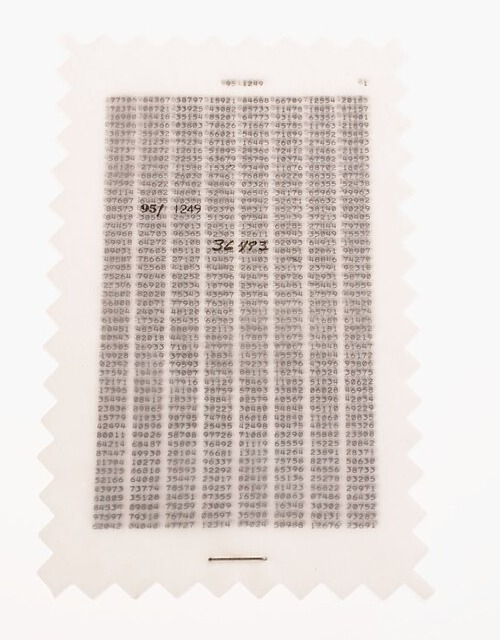
\includegraphics[width=\linewidth,height=5.2cm,keepaspectratio]{figs/photos/ch13_otp_photo}
\caption{A one-time pad sheet: columns of random digit groups, each to be used once and
destroyed.\mdccredit{ch13_otp_photo}}
\label{fig:ch13_otp_photo}\end{minipage}\hfill
\begin{minipage}[t]{0.55\linewidth}\centering
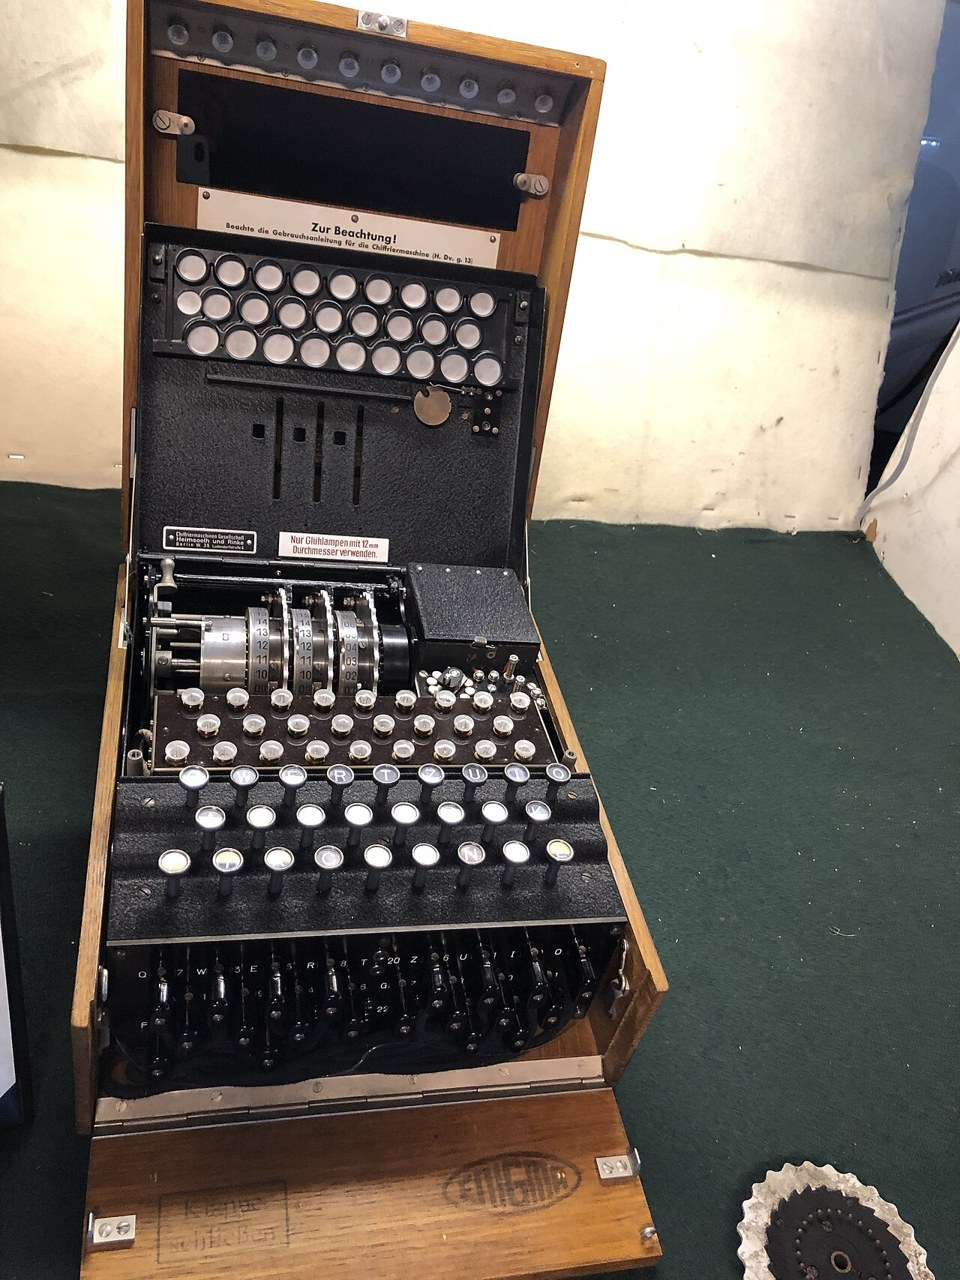
\includegraphics[width=\linewidth,height=5.2cm,keepaspectratio]{figs/photos/ch13_enigma}
\caption{An Enigma machine. Its key (rotor order, settings and plugboard) is short and reused for
a whole day's traffic, so by Shannon's theorem it cannot be perfectly secret; Allied codebreakers
proved the point.\mdccredit{ch13_enigma}}
\label{fig:ch13_enigma}\end{minipage}
\end{figure}

\begin{history}[Venona: the price of reusing a pad]
The one-time pad's weakness is operational, not mathematical: the key must be as long as all the
traffic, truly random, secretly delivered and never reused. Producing that much key material in
wartime was hard, and some Soviet one-time-pad pages were duplicated and used twice during the
Second World War. US Army codebreakers in the \emph{Venona} project, begun in 1943, exploited the
reuse and over the following decades were able to read parts of thousands of messages. The
mathematics of Figure~\ref{fig:ch13_onetimepad} is exactly what they faced: two ciphertexts with a
common key reveal the combination of two plaintexts, and natural language has enough redundancy
(Section~\ref{sec:ch13:entropy}) to pull the combination apart.
\end{history}

\subsection{The wiretap channel}

Aaron Wyner's 1975 \term{wiretap channel} changed the question. Alice sends to Bob over a channel,
and an eavesdropper Eve receives a \emph{noisier} version. Without any shared key, Alice can
send messages that Bob decodes reliably while Eve learns essentially nothing, at rates up to the
\term{secrecy capacity}; for the Gaussian case (Leung-Yan-Cheong and Hellman, 1978)
\begin{equation}
C_s=\Big[\log_2(1+\mathrm{SNR}_{\text{Bob}})-\log_2(1+\mathrm{SNR}_{\text{Eve}})\Big]^+.
\label{eq:ch13:wiretap}
\end{equation}
In words: secrecy is the information advantage Bob has over Eve. The coding idea is randomised
binning: Alice uses a code of rate close to Bob's capacity, but spends the part of it that Eve
could decode on random ``confusion'' bits, so that Eve's observation is consistent with every
possible secret message. If Bob's SNR is 20\,dB and Eve's 10\,dB, $C_s=6.66-3.46=3.2$\,bits/s/Hz
can be sent in perfect secrecy, with no key at all (the red dot in Figure~\ref{fig:ch13_secrecy}).

\begin{figure}[htbp]\centering
\begin{tikzpicture}[node distance=0.55cm and 0.7cm,
  blk/.style={draw=navy,fill=navy!6,thick,minimum height=0.9cm,minimum width=1.5cm,align=center,font=\sffamily\scriptsize},
  eve/.style={draw=accent,fill=accent!6,thick,minimum height=0.9cm,minimum width=1.5cm,align=center,font=\sffamily\scriptsize},
  arr/.style={-{Stealth[length=2mm]},thick,navy}]
\node[blk] (a) {Alice\\encoder};
\node[blk,right=1.1cm of a] (ch) {Main channel\\$\mathrm{SNR}_{\text{B}}$};
\node[blk,right=of ch] (b) {Bob\\decoder};
\node[eve,below=0.55cm of ch] (ech) {Eve's channel\\$\mathrm{SNR}_{\text{E}}<\mathrm{SNR}_{\text{B}}$};
\node[eve,right=of ech] (e) {Eve};
\node[left=0.5cm of a,font=\sffamily\scriptsize] (m) {$M$};
\node[right=0.5cm of b,font=\sffamily\scriptsize] (mh) {$\hat M$};
\node[right=0.5cm of e,font=\sffamily\scriptsize,text=accent,align=left] {$I(M;Z^n)/n\to0$};
\draw[arr] (m) -- (a); \draw[arr] (a) -- node[above,font=\scriptsize]{$X^n$} (ch);
\draw[arr] (ch) -- (b); \draw[arr] (b) -- (mh);
\draw[arr,accent] ([xshift=0.55cm]a.east) |- (ech); \draw[arr,accent] (ech) -- node[above,font=\scriptsize]{$Z^n$} (e);
\end{tikzpicture}
\caption{Wyner's wiretap channel. The eavesdropper sees a degraded copy of the transmission.
Coding can make Bob's error probability and Eve's information about the message both vanish, at
rates up to the secrecy capacity~\eqref{eq:ch13:wiretap}.}
\label{fig:ch13_wiretap}
\end{figure}

\mdcfig[0.5]{ch13_secrecy}{Secrecy capacity~\eqref{eq:ch13:wiretap} against Bob's SNR for three
eavesdroppers. Each curve is Bob's capacity shifted down by Eve's; secrecy appears only when Bob's
channel is the better one.}

Figure~\ref{fig:ch13_secrecy} shows the shape of the result. Secrecy capacity is zero until Bob's
SNR overtakes Eve's, and then it grows exactly as fast as Bob's own capacity: every extra decibel
Bob has over Eve is converted, at the high-SNR rate of a third of a bit per decibel, into secret
bits. Notice what the curves do not depend on: neither Alice nor Bob needs a shared key, a
computational assumption or a trusted third party. Secrecy comes from physics alone, from the fact
that Bob is better placed than Eve. That is both the beauty and, as the pitfall explains, the
practical weakness of the idea: everything hinges on knowing how well Eve can listen.

\begin{pitfall}[Physical-layer security needs a model of Eve]
Equation~\eqref{eq:ch13:wiretap} requires Alice to know, or bound, Eve's SNR. A passive eavesdropper
with a large antenna, or simply standing closer, breaks the assumption, and in practice nobody can
certify an adversary's receiver. That is why \emph{physical-layer security} has seen limited
deployment compared with cryptography, and why its most practical descendants use the channel for
something else: generating shared secret keys from the reciprocal randomness of a fading channel
that only Alice and Bob observe (Maurer, 1993), or quantum key distribution, in which the laws of
physics, rather than an SNR assumption, reveal an eavesdropper. In both cases the key then feeds a
conventional or one-time-pad cipher---Shannon's 1949 framework, completed.
\end{pitfall}

%======================================================================
\section{Where practical systems stand}
\label{sec:ch13:today}
%======================================================================

\mdcfig{ch13_chase}{Fifty years of approaching Shannon's limit at a code rate near $\frac12$ on the
binary-input Gaussian channel: the $E_b/N_0$ required for a bit error rate of about $10^{-5}$
(the 2001 LDPC point is at $10^{-6}$). The Voyager concatenated system ran at rate 0.44 rather
than 0.5. Values are the widely quoted approximate figures from the original papers and the survey
by Costello and Forney. The dashed line is the limit for binary inputs at rate $\frac12$ (0.19\,dB);
the dotted line is the ultimate limit for any rate.}

\begin{table}[htbp]\centering\small
\caption{Approximate gap to capacity of representative systems. ``Limit'' says which bound the gap
is measured against. Values are rounded engineering estimates from the sources cited in the text and
Further Reading.}
\label{tab:ch13:gaps}
\begin{tabularx}{\linewidth}{@{}l>{\raggedright\arraybackslash}Xlr@{}}
\toprule
System & Code and operating point & Limit & Gap \\
\midrule
Uncoded QPSK/QAM & $P_b=10^{-5}$ & Shannon & 8--10\,dB \\
$K=7$ convolutional & rate $\frac12$, soft Viterbi, $P_b=10^{-5}$ & binary input & $\approx4.2$\,dB \\
Voyager (1977) & RS(255,223) + $K=7$, rate 0.44, $P_b=10^{-5}$ & binary input & $\approx2.6$\,dB \\
Turbo code (1993) & rate $\frac12$, 65\,536-bit interleaver, $P_b=10^{-5}$ & binary input & $\approx0.5$\,dB \\
LDPC (2001) & rate $\frac12$, $n=10^7$, $P_b=10^{-6}$ & binary input & $\approx0.04$\,dB \\
DVB-S2 & QPSK $\frac12$, 64\,800-bit LDPC, QEF & Shannon & 1.1\,dB \\
DVB-S2 & 32APSK 9/10, 64\,800-bit LDPC, QEF & Shannon & 2.9\,dB \\
5G NR data & LDPC, several thousand bits, 10\% BLER & finite length & about 1\,dB \\
5G NR control & CRC-aided polar, tens of bits & finite length & $<1$\,dB \\
URLLC packet & 256 bits, $\epsilon=10^{-5}$ & Shannon (asymptotic) & $\ge1.8$\,dB \\
\bottomrule
\end{tabularx}
\end{table}

\begin{history}[The fifty-year chase]
Shannon's theorem told engineers in 1948 that at rate $\frac12$ on a Gaussian channel with binary
inputs, reliable communication is possible down to $E_b/N_0=0.19$\,dB. Uncoded BPSK needed 9.6\,dB
for a bit error rate of $10^{-5}$: a gap of more than 9\,dB. Closing it took half a century.
Hamming (1950) and Golay (1949) found the first error-correcting codes; Reed and Muller (1954) and
Reed and Solomon (1960) gave algebraic families. Algebraic codes with hard-decision decoding gained
only a few decibels, and for two decades the leading practical approach was \emph{probabilistic}:
convolutional codes with sequential decoding (Wozencraft 1957, Fano 1963), which flew on Pioneer~9
in 1968, and then Viterbi's 1967 maximum-likelihood algorithm, whose $K=7$, rate-$\frac12$ code with
soft decisions needs about 4.4\,dB and became the workhorse of satellite and space communication.
Forney's concatenated codes (1966) put a Reed--Solomon outer code around it; on Voyager this
combination reached about 2.5\,dB. Mariner's 1969 Reed--Muller code, Ungerboeck's trellis-coded
modulation (1982) for bandwidth-limited modems, and the Galileo mission's giant $K=15$ decoder filled
in the story.

Then, in 1993, Claude Berrou, Alain Glavieux and Punya Thitimajshima reported \emph{turbo codes}
reaching $10^{-5}$ at 0.7\,dB---half a decibel from the limit. The coding community's first
reaction was disbelief; within a few years the results had been reproduced everywhere. David MacKay
and Radford Neal (1996) rediscovered Gallager's LDPC codes and showed they were as good; Tom
Richardson and R\"udiger Urbanke developed density evolution to design them; and in 2001 Chung,
Forney, Richardson and Urbanke simulated an irregular LDPC code of block length $10^7$ within
0.04\,dB of the limit, with a design threshold within 0.0045\,dB. Erdal Ar{\i}kan's polar codes (2009)
were the first provably capacity-achieving codes with low-complexity encoding and decoding. The chase
was over; the remaining work is about latency, complexity, short blocks and power consumption.
\end{history}

Figure~\ref{fig:ch13_chase} is the fifty-year chase in one picture, and it has the shape of every
great engineering story: a long, slow grind of a decibel per decade, then a sudden collapse when a
new idea arrives. Each step had a customer waiting. The deep-space programme paid for the
convolutional and concatenated codes, because every decibel there is worth a quarter more pictures;
voice-band modems paid for trellis-coded modulation, because every decibel there was worth another
few kilobits per second to millions of subscribers; and mobile and broadcast systems paid for turbo
and LDPC codes, because every decibel there is worth a smaller cell or a smaller dish.

Table~\ref{tab:ch13:gaps} summarises where representative systems sit today. The figures are
indicative: a gap depends on the block length, the error-rate target and which limit is used
(Gaussian-input, constellation-constrained or finite-blocklength), and the table says which.

\begin{figure}[htbp]\centering
\begin{tikzpicture}[nb/.style={draw=navy,fill=navy!5,thick,rounded corners=3pt,minimum width=3.3cm,minimum height=1.55cm,align=center,font=\sffamily\scriptsize}]
\foreach \x/\y/\n/\t in {0/0/1 bit/a fair coin toss,
                         3.6/0/4.75 $\to$ $\approx$1/bits per letter of English,
                         7.2/0/$1-h(p)$/capacity of a BSC,
                         10.8/0/$B\log_2(1+\mathrm{SNR})$/the AWGN channel,
                         0/-1.8/$-1.59$\,dB/the Shannon limit,
                         3.6/-1.8/1.53\,dB/the shaping gain,
                         7.2/-1.8/6.02\,dB/per bit of fidelity,
                         10.8/-1.8/0.0045\,dB/LDPC's distance to the limit}
  \node[nb] at (\x,\y) {{\large\bfseries\color{accent}\n}\\[2pt]\t};
\end{tikzpicture}
\caption{Information theory in eight numbers. Each is derived in this chapter and each shows up,
sooner or later, in the design of a real system.}
\label{fig:ch13_numbers}
\end{figure}

\begin{keyidea}[Where the remaining decibels are]
For long blocks on a stationary Gaussian channel, the coding problem is solved: modern codes sit a
few tenths of a decibel to one decibel from capacity. The decibels that remain in real systems are
elsewhere: in short packets (finite blocklength), in constellations used near saturation or
without shaping (up to 1.53\,dB), in bit-wise decoding (BICM, a few tenths), in channel estimation
and synchronisation, in overheads, and in the margins that protect against a channel that changes.
The frontier of information theory in practice has moved from ``can we reach capacity?'' to ``can
we reach it with short blocks, low latency, low power and many users?''---and, at the system level,
to the capacity of networks, where most questions remain open.
\end{keyidea}

%======================================================================
\section{Summary}
%======================================================================

Figure~\ref{fig:ch13_numbers} collects the chapter's most important numbers; the list below
collects its ideas.

\begin{itemize}
\item Information is surprise, measured by probability: an outcome of probability $p$ carries
$\log_2(1/p)$ bits, and a source's entropy $H=-\sum p\log_2p$ is its average information---the
number of yes/no questions the best questioner needs. English text carries roughly 1 bit per
character of a possible 4.75; sources with memory are described by their entropy rate.
\item Joint and conditional entropies obey the chain rule; relative entropy $D(p\|q)\ge0$ underlies
almost every inequality; mutual information $I(X;Y)=H(X)-H(X\mid Y)$ measures what gets through a
channel. Processing cannot increase it (data-processing inequality), and Fano's inequality turns
residual uncertainty into a lower bound on error probability.
\item The AEP: long sequences are almost surely typical, about $2^{nH}$ of them, each of probability
about $2^{-nH}$. Hence the source coding theorem (compress to $H$, no further), the Kraft inequality
and Huffman coding within one bit of $H$.
\item A DMC has capacity $C=\max I(X;Y)$: $1-h(p)$ for the BSC, $1-p$ for the BEC. Blahut--Arimoto
computes it in general. The channel coding theorem makes every rate below $C$ achievable with
vanishing error probability, via random coding and joint typicality, and none above it (converse
via Fano).
\item The error probability falls as $2^{-nE_r(R)}$; at finite length the achievable rate is
$C-\sqrt{V/n}\,\Q^{-1}(\epsilon)$, a penalty of several decibels for packets of a few hundred bits.
\item The Gaussian maximises entropy for a given variance, so Gaussian noise is the worst noise and a
Gaussian input the best input. The AWGN channel has $C=B\log_2(1+\mathrm{SNR})$, derived by packing
noise spheres; capacity is logarithmic in power at high SNR and linear at low SNR, and no system can
work below $E_b/N_0=-1.59$\,dB.
\item Finite constellations follow Shannon's curve until they saturate; uniform square QAM loses up to
1.53\,dB (shaping); BICM with Gray labels loses little when constellations are used near their
upper range.
\item Parallel channels call for water-filling, realised as bit loading in DMT and OFDM. Fading costs
little capacity when codes span many fades (ergodic capacity) but a great deal when they do not
(outage), which diversity repairs. MIMO multiplies the high-SNR slope by $\min(n_t,n_r)$.
\item Multi-user channels have capacity regions: SIC achieves the MAC region, superposition coding
the degraded broadcast region, and dirty-paper coding the MIMO downlink.
\item Rate--distortion theory gives the bits needed for a given fidelity: 6.02\,dB per bit for a
Gaussian source, with scalar quantisers 1.53 to 4.35\,dB short. Perfect secrecy needs a key as long
as the message, unless the eavesdropper's channel is worse.
\end{itemize}

\begin{labbox}[Information theory, live]
Lab 19, \lab{moderncomms-labs/labs/lab19\_information\_theory.py} (run it with
\lab{python lab19\_information\_theory.py}), turns this chapter into a set of interactive
experiments:
\begin{itemize}
\item \textbf{Surprise and entropy}: a biased coin and a two-state Markov sensor; the binary entropy
curve, the surprise of each report and the saving that memory buys (Section~\ref{sec:ch13:entropy}).
\item \textbf{Entropy of text and images}: type or paste text, or pick a built-in image; see letter histograms,
the $F_0$--$F_3$ staircase, compressor results (Figures~\ref{fig:ch13_letter_freq}
and~\ref{fig:ch13_compressors}) and the entropy of pixels versus pixel differences
(Figure~\ref{fig:ch13_image_entropy}).
\item \textbf{Huffman coding}: drag symbol probabilities, watch the tree rebuild, and compare the
average length with the bound~\eqref{eq:ch13:lbound}, symbol by symbol and in pairs.
\item \textbf{DMC capacity}: edit a transition matrix (or pick BSC, BEC or Z) and watch
Blahut--Arimoto converge, as in Figure~\ref{fig:ch13_dmc_capacity}.
\item \textbf{Shannon's AWGN limit}: received $P/N_0$, bandwidth and your data rate on the
capacity-versus-bandwidth curve and the bandwidth--power plane (Section~\ref{sec:ch13:plane}).
\item \textbf{Constrained capacity}: coded-modulation and BICM capacities of the constellations in
\texttt{commlib.modulation} against Shannon, with Gray or natural labels and hard- versus
soft-decision BPSK (Figures~\ref{fig:ch13_constrained} and~\ref{fig:ch13_bicm}).
\item \textbf{Finite blocklength}: the normal approximation~\eqref{eq:ch13:normal} with sliders for
$n$, $\epsilon$ and SNR (Figure~\ref{fig:ch13_finite_blocklength}).
\item \textbf{Water-filling}: draggable sub-channel SNRs, a total-power slider, the water level and
gap-based bit loading (Figure~\ref{fig:ch13_waterfilling}), plus a 256-tone DSL line.
\item \textbf{Rate--distortion}: uniform, Lloyd--Max and entropy-coded quantisers against the
Gaussian rate--distortion bound, and reverse water-filling (Section~\ref{sec:ch13:rd}).
\end{itemize}
The figure script \lab{book/figscripts/ch13\_figs.py} computes every data figure in this chapter and
contains compact, reusable implementations of all of these.
\end{labbox}

\problems
\begin{enumerate}[label=\thechapter.\arabic*]
\item A loaded die shows 1 with probability $\frac12$ and each of 2--6 with probability
$\frac1{10}$. Compute its entropy and compare it with that of a fair die. Design a Huffman code for a
single throw and find its average length. How close can you get to the entropy by coding pairs of
throws?
\item Using Gibbs' inequality, prove that $H(X)\le\log_2|\mathcal{X}|$ and that $H(Y\mid X)\le H(Y)$.
When is each an equality?
\item A three-state Markov source has transition matrix with rows $(0.8,0.1,0.1)$,
$(0.2,0.6,0.2)$ and $(0.25,0.25,0.5)$. Find its stationary distribution, its entropy rate and the
entropy of its stationary marginal. By what percentage does a coder that exploits the memory beat one
that does not?
\item Show that $I(X;Y)=D\big(p(x,y)\|p(x)p(y)\big)$ and hence that $I(X;Y)\ge0$. Give an example in
which $I(X;Y\mid Z)>I(X;Y)$ and one in which $I(X;Y\mid Z)<I(X;Y)$.
\item Two BSCs with crossover probabilities $p_1$ and $p_2$ are connected in series. Show that the
cascade is a BSC and find its crossover probability. Verify the data-processing inequality by
comparing capacities for $p_1=p_2=0.05$.
\item Derive the Z-channel capacity~\eqref{eq:ch13:z} and the optimal input probability. Show that the
optimum $\Pr(X=1)$ is always between $1/e$ and $\frac12$.
\item A binary code has 16 codewords of length 7 and corrects every single error (the Hamming code).
Show that its Hamming spheres of radius 1 exactly fill the space $\{0,1\}^7$. Use the sphere-packing
argument to show that no code of length 7 and more than 16 codewords can correct all single errors.
\item Using the normal approximation~\eqref{eq:ch13:normal}, estimate the largest number of information
bits that can be sent in $n=1000$ uses of a BSC with $p=0.11$ at a block error probability of
$10^{-3}$. Compare with $nC$.
\item Starting from~\eqref{eq:ch13:shannonhartley}, derive $C_\infty$ and the Shannon limit. Find the
minimum $E_b/N_0$ at spectral efficiencies of 0.1, 0.5, 4 and 8\,bits/s/Hz.
\item An ADSL tone at 4.3125\,kHz spacing and 4000 DMT symbols per second has an SNR of 38\,dB. With a
gap of 9.8\,dB, a coding gain of 4\,dB and a margin of 6\,dB, how many bits does it carry, and what is
the capacity of the tone? How many such tones are needed for 8\,Mb/s?
\item Three parallel channels have noise variances 1, 2 and 5 and share a total power of 4. Find the
water-filling allocation and the capacity. Repeat for total powers of 1 and 12, and interpret.
\item For Rayleigh fading, show that at high SNR the ergodic capacity is
$\log_2\bar\gamma-\gamma_{\mathrm{E}}\log_2e$. Find the SNR at which the 1\%-outage capacity reaches
2\,bits/s/Hz with one, two and four diversity branches.
\item For the two-user Gaussian MAC with $P_1/N=10$ and $P_2/N=3$, compute the corners of the capacity
region. Show that FDMA with bandwidth fractions proportional to the powers achieves the maximum sum
rate.
\item A Gaussian source is sent over an AWGN channel with SNR 20\,dB, one channel use per source
sample. Compute the minimum mean-square distortion (a) with optimal digital coding, (b) with uncoded
analog transmission, and (c) with 64-QAM carrying 3 bits per real dimension of an 8-level Lloyd--Max
quantiser. Explain the result.
\item Bob receives Alice at 15\,dB. Eve receives her at 5\,dB, 15\,dB or 25\,dB. What is the secrecy
capacity in each case? What does a one-time pad require instead?
\item \emph{(Simulation)} Implement the Blahut--Arimoto algorithm and use it to compute the capacity of
BPSK in AWGN with the matched-filter output quantised to 1, 2, 3 and 4 bits (uniform thresholds you
optimise). At rate $\frac12$, how many decibels does each quantiser lose relative to unquantised soft
decisions?
\item \emph{(Simulation)} Reproduce Figure~\ref{fig:ch13_bicm} by Monte Carlo using
\texttt{Constellation.llr} from \texttt{commlib}: compute $\sum_iI(B_i;Y)$ from the exact LLRs, and
compare Gray and natural labelling on 64-QAM. Then repeat with the max-log LLRs and measure the loss.
\item \emph{(Simulation)} Estimate the entropy of a long English text file using single-letter,
digram and trigram statistics, and compare with the compression ratios of \texttt{zlib},
\texttt{bz2} and \texttt{lzma}. Which estimate is closest to Shannon's range, and why do all of them
exceed it?
\end{enumerate}

\furtherreading
\begin{itemize}
\item C.~E.~Shannon, ``A mathematical theory of communication,'' \emph{Bell System Technical Journal},
vol.~27, pp.~379--423 and 623--656, 1948; and ``Communication in the presence of noise,''
\emph{Proc. IRE}, vol.~37, no.~1, pp.~10--21, 1949. Both remain readable and surprisingly modern;
the second contains the sphere-packing derivation and the sampling theorem.
\item C.~E.~Shannon, ``Prediction and entropy of printed English,'' \emph{Bell System Technical
Journal}, vol.~30, pp.~50--64, 1951; and ``Communication theory of secrecy systems,'' \emph{Bell
System Technical Journal}, vol.~28, pp.~656--715, 1949.
\item T.~M.~Cover and J.~A.~Thomas, \emph{Elements of Information Theory}, 2nd ed., Wiley, 2006. The
standard graduate text: typicality, channel capacity, Gaussian channels, rate--distortion and network
information theory, with clear proofs.
\item R.~G.~Gallager, \emph{Information Theory and Reliable Communication}, Wiley, 1968. The classic
engineering treatment, and the source for error exponents.
\item D.~J.~C.~MacKay, \emph{Information Theory, Inference, and Learning Algorithms}, Cambridge
University Press, 2003. An inspiring, example-driven book that connects information theory with
modern codes and machine learning; freely available from the author's website.
\item A.~El~Gamal and Y.-H.~Kim, \emph{Network Information Theory}, Cambridge University Press, 2011.
The definitive treatment of multiple-access, broadcast, interference, relay and wiretap channels.
\item D.~Tse and P.~Viswanath, \emph{Fundamentals of Wireless Communication}, Cambridge University
Press, 2005. Capacity of fading and MIMO channels, outage, diversity--multiplexing trade-off and
multi-user capacity, with the engineer's intuition always in front.
\item Y.~Polyanskiy, H.~V.~Poor and S.~Verd\'u, ``Channel coding rate in the finite blocklength
regime,'' \emph{IEEE Transactions on Information Theory}, vol.~56, no.~5, pp.~2307--2359, 2010.
\item G.~D.~Forney, Jr.\ and G.~Ungerboeck, ``Modulation and coding for linear Gaussian channels,''
\emph{IEEE Transactions on Information Theory}, vol.~44, no.~6, pp.~2384--2415, 1998. Shaping gain,
the SNR gap and the practical path to capacity on band-limited channels.
\item G.~Caire, G.~Taricco and E.~Biglieri, ``Bit-interleaved coded modulation,'' \emph{IEEE
Transactions on Information Theory}, vol.~44, no.~3, pp.~927--946, 1998.
\item D.~J.~Costello, Jr.\ and G.~D.~Forney, Jr., ``Channel coding: the road to channel capacity,''
\emph{Proceedings of the IEEE}, vol.~95, no.~6, pp.~1150--1177, 2007. The fifty-year chase, told by
two of its participants, with the numbers behind Figure~\ref{fig:ch13_chase}.
\item S.~Verd\'u, ``Fifty years of Shannon theory,'' \emph{IEEE Transactions on Information Theory},
vol.~44, no.~6, pp.~2057--2078, 1998; and J.~Soni and R.~Goodman, \emph{A Mind at Play: How Claude
Shannon Invented the Information Age}, Simon \& Schuster, 2017. A scholarly history of the field and
a lively biography of its founder, including Theseus, the juggling machines and the unicycle.
\end{itemize}
